\documentclass[twoside]{book}

% Packages required by doxygen
\usepackage{fixltx2e}
\usepackage{calc}
\usepackage{doxygen}
\usepackage[export]{adjustbox} % also loads graphicx
\usepackage{graphicx}
\usepackage[utf8]{inputenc}
\usepackage{makeidx}
\usepackage{multicol}
\usepackage{multirow}
\PassOptionsToPackage{warn}{textcomp}
\usepackage{textcomp}
\usepackage[nointegrals]{wasysym}
\usepackage[table]{xcolor}

% NLS support packages
\usepackage{hfont}

% Font selection
\usepackage[T1]{fontenc}
\usepackage[scaled=.90]{helvet}
\usepackage{courier}
\usepackage{amssymb}
\usepackage{sectsty}
\renewcommand{\familydefault}{\sfdefault}
\allsectionsfont{%
  \fontseries{bc}\selectfont%
  \color{darkgray}%
}
\renewcommand{\DoxyLabelFont}{%
  \fontseries{bc}\selectfont%
  \color{darkgray}%
}
\newcommand{\+}{\discretionary{\mbox{\scriptsize$\hookleftarrow$}}{}{}}

% Page & text layout
\usepackage{geometry}
\geometry{%
  a4paper,%
  top=2.5cm,%
  bottom=2.5cm,%
  left=2.5cm,%
  right=2.5cm%
}
\tolerance=750
\hfuzz=15pt
\hbadness=750
\setlength{\emergencystretch}{15pt}
\setlength{\parindent}{0cm}
\setlength{\parskip}{3ex plus 2ex minus 2ex}
\makeatletter
\renewcommand{\paragraph}{%
  \@startsection{paragraph}{4}{0ex}{-1.0ex}{1.0ex}{%
    \normalfont\normalsize\bfseries\SS@parafont%
  }%
}
\renewcommand{\subparagraph}{%
  \@startsection{subparagraph}{5}{0ex}{-1.0ex}{1.0ex}{%
    \normalfont\normalsize\bfseries\SS@subparafont%
  }%
}
\makeatother

% Headers & footers
\usepackage{fancyhdr}
\pagestyle{fancyplain}
\fancyhead[LE]{\fancyplain{}{\bfseries\thepage}}
\fancyhead[CE]{\fancyplain{}{}}
\fancyhead[RE]{\fancyplain{}{\bfseries\leftmark}}
\fancyhead[LO]{\fancyplain{}{\bfseries\rightmark}}
\fancyhead[CO]{\fancyplain{}{}}
\fancyhead[RO]{\fancyplain{}{\bfseries\thepage}}
\fancyfoot[LE]{\fancyplain{}{}}
\fancyfoot[CE]{\fancyplain{}{}}
\fancyfoot[RE]{\fancyplain{}{\bfseries\scriptsize 다음에 의해 생성됨 \+:  Doxygen }}
\fancyfoot[LO]{\fancyplain{}{\bfseries\scriptsize 다음에 의해 생성됨 \+:  Doxygen }}
\fancyfoot[CO]{\fancyplain{}{}}
\fancyfoot[RO]{\fancyplain{}{}}
\renewcommand{\footrulewidth}{0.4pt}
\renewcommand{\chaptermark}[1]{%
  \markboth{#1}{}%
}
\renewcommand{\sectionmark}[1]{%
  \markright{\thesection\ #1}%
}

% Indices & bibliography
\usepackage{natbib}
\usepackage[titles]{tocloft}
\setcounter{tocdepth}{3}
\setcounter{secnumdepth}{5}
\makeindex

% Hyperlinks (required, but should be loaded last)
\usepackage{ifpdf}
\ifpdf
  \usepackage[pdftex,pagebackref=true]{hyperref}
\else
  \usepackage[ps2pdf,pagebackref=true]{hyperref}
\fi
\hypersetup{%
  colorlinks=true,%
  linkcolor=blue,%
  citecolor=blue,%
  unicode%
}

% Custom commands
\newcommand{\clearemptydoublepage}{%
  \newpage{\pagestyle{empty}\cleardoublepage}%
}

\usepackage{caption}
\captionsetup{labelsep=space,justification=centering,font={bf},singlelinecheck=off,skip=4pt,position=top}

%===== C O N T E N T S =====

\begin{document}

% Titlepage & ToC
\hypersetup{pageanchor=false,
             bookmarksnumbered=true,
             pdfencoding=unicode
            }
\pagenumbering{alph}
\begin{titlepage}
\vspace*{7cm}
\begin{center}%
{\Large S\+L\+T\+E\+CH \& Simple\+H\+AN \\[1ex]\large 1.\+0.\+0 }\\
\vspace*{1cm}
{\large 다음에 의해 생성됨 \+:  Doxygen 1.8.14}\\
\end{center}
\end{titlepage}
\clearemptydoublepage
\pagenumbering{roman}
\tableofcontents
\clearemptydoublepage
\pagenumbering{arabic}
\hypersetup{pageanchor=true}

%--- Begin generated contents ---
\chapter{C\+A\+N\+A\+D\+A향 L\+C\+D형 E\+S\+P-\/12E 모듈 개발}
\label{index}\hypertarget{index}{}E\+S\+P8266 Arduino core환경 개발~\newline
이 프로젝트 자세한 내용 정리를 위한 개발 문서입니다 \begin{DoxyAuthor}{작성자}
Goodbro(\+C\+T\+O) 이우섭 
\end{DoxyAuthor}
\begin{DoxyDate}{날짜}
2018.\+08.\+06
\end{DoxyDate}
\begin{DoxyItemize}
\item Wifi Module $>$ Wall Pad \tabulinesep=1mm
\begin{longtabu} spread 0pt [c]{*{2}{|X[-1]}|}
\hline
\rowcolor{\tableheadbgcolor}\textbf{ F\+CU  }&\textbf{ E\+RV   }\\\cline{1-2}
\endfirsthead
\hline
\endfoot
\hline
\rowcolor{\tableheadbgcolor}\textbf{ F\+CU  }&\textbf{ E\+RV   }\\\cline{1-2}
\endhead
Header~\newline
 init \+: 0x\+F5~\newline
 상태응답 \+: 0x\+D5~\newline
 제어응답 \+: 0\+X\+C5  &Header~\newline
 상태응답 \+: 0x\+D7~\newline
 제어응답 \+: 0\+X\+C7   \\\cline{1-2}
Wifi감도~\newline
 중단($<$-\/85) \+: 0x01~\newline
 연결1($<$-\/75) \+: 0x02~\newline
 연결2($>$ -\/75) \+: 0x03  &Wifi감도~\newline
 F\+C\+U와 동일   \\\cline{1-2}
Mode \& Fan 속도~\newline
 M\+SB \mbox{[}냉방 \+: 0x00\mbox{]} \mbox{[}난방 \+: 0x10\mbox{]} \mbox{[}송풍 \+: 0x20\mbox{]} +\+Fan 자동 \+: 0x80~\newline
 L\+SB \mbox{[}Off \+: 0x00\mbox{]} \mbox{[}Low \+: 0x01\mbox{]} \mbox{[}Mid \+: 0x02\mbox{]} \mbox{[}High \+: 0x03\mbox{]}  &Mode~\newline
 Vent \+: 0x00~\newline
 Eco \+: 0x01~\newline
 Timer \+: 0x02~\newline
 By\+Pass \+: 0x03   \\\cline{1-2}
F\+L\+AG~\newline
 7bit \+: Remote lock~\newline
 6bit \+: Mode event~\newline
 3bit \+: Timer 비/가동~\newline
 1bit\+: 화씨/섭씨~\newline
 0bit \+: 가동신호  &Fan 속도~\newline
 Off \+: 0x00~\newline
 Low \+: 0x01~\newline
 Mid \+: 0x02~\newline
 High \+: 0x03   \\\cline{1-2}
온도세팅@ 7bit \+: .5도~\newline
 0$\sim$6bit \+: 0$\sim$127도  &F\+L\+AG~\newline
 7bit \+: Remote lock~\newline
 6bit \+: Mode event~\newline
 3bit \+: Timer 비/가동~\newline
 2bit \+: Heater off/on~\newline
 1bit \+: 화씨/섭씨~\newline
 0bit \+: 가동신호   \\\cline{1-2}
Wifi Status~\newline
 AP \& 중단 \+: 0x00~\newline
 Wifi \& 중단 \+: 0x10~\newline
 Wifi \& 연결 \+: 0x11  &Wifi Status~\newline
 F\+C\+U와 동일   \\\cline{1-2}
E\+C\+O\+DE~\newline
 내부통신에러 \+: 0x01  &E\+C\+O\+DE~\newline
 F\+C\+U와 동일   \\\cline{1-2}
Check\+Sum  &Check\+Sum   \\\cline{1-2}
\end{longtabu}
\end{DoxyItemize}
\begin{DoxyItemize}
\item Wifi Module $<$ Wall Pad \tabulinesep=1mm
\begin{longtabu} spread 0pt [c]{*{2}{|X[-1]}|}
\hline
\rowcolor{\tableheadbgcolor}\textbf{ F\+CU  }&\textbf{ E\+RV   }\\\cline{1-2}
\endfirsthead
\hline
\endfoot
\hline
\rowcolor{\tableheadbgcolor}\textbf{ F\+CU  }&\textbf{ E\+RV   }\\\cline{1-2}
\endhead
Header~\newline
 init \+: 0x\+E5~\newline
 상태응답 \+: 0x\+B5~\newline
 제어응답 \+: 0\+X\+A5  &Header~\newline
 상태응답 \+: 0x\+B7~\newline
 제어응답 \+: 0\+X\+A7   \\\cline{1-2}
현재온도 (소수점)  &현재온도 (소수점)   \\\cline{1-2}
Mode \& Fan 속도~\newline
 M\+SB \mbox{[}냉방 \+: 0x00\mbox{]} \mbox{[}난방 \+: 0x10\mbox{]} \mbox{[}송풍 \+: 0x20\mbox{]} +\+Fan 자동 \+: 0x80~\newline
 L\+SB \mbox{[}Off \+: 0x00\mbox{]} \mbox{[}Low \+: 0x01\mbox{]} \mbox{[}Mid \+: 0x02\mbox{]} \mbox{[}High \+: 0x03\mbox{]}  &Mode~\newline
 Vent \+: 0x00~\newline
 Eco \+: 0x01~\newline
 Timer \+: 0x02~\newline
 By\+Pass \+: 0x03   \\\cline{1-2}
F\+L\+AG~\newline
 7bit \+: Remote lock~\newline
 6bit \+: 팬 가동상태~\newline
 5bit \+: 실내온도 센서(R\+C센서/리턴제어)~\newline
 4bit \+: Pipe 개수(2/4)~\newline
 3bit \+: 현재온도(양수/음수)~\newline
 2bit \+: 동파방지 비/가동~\newline
 1bit\+: 화씨/섭씨~\newline
 0bit \+: 가동신호  &Fan 속도~\newline
 Off \+: 0x00~\newline
 Low \+: 0x01~\newline
 Mid \+: 0x02~\newline
 High \+: 0x03   \\\cline{1-2}
온도세팅@ 7bit \+: .5도~\newline
 0$\sim$6bit \+: 0$\sim$127도  &F\+L\+AG~\newline
 7bit \+: Remote lock~\newline
 6bit \+: Mode event~\newline
 4bit \+: Filter교체알람~\newline
 3bit \+: 현재온도(양수/음수)~\newline
 2bit \+: Heater off/on~\newline
 1bit \+: 화씨/섭씨~\newline
 0bit \+: 가동신호   \\\cline{1-2}
현재온도 (정수)  &현재온도 (정수)   \\\cline{1-2}
E\+C\+O\+DE~\newline
 내부통신에러 \+: 0x01~\newline
 R/\+C온도센서에러 \+: 0x02~\newline
 동파방지센서에러 \+: 0x04~\newline
 Pipe1온도센서에러 \+: 0x08~\newline
 Air센서에러 \+: 0x10~\newline
 수위센서에러 \+: 0x20~\newline
 Pipe2온도센서에러 \+:0x40~\newline
 Fan(\+B\+L\+D\+C)에러 \+: 0x80  &E\+C\+O\+DE~\newline
 내부통신에러 \+: 0x01~\newline
 실내온도에러 \+: 0x08~\newline
 외기온도에러 \+: 0x10~\newline
 Fan(\+B\+L\+D\+C)에러 \+: 0x80   \\\cline{1-2}
Check\+Sum  &Check\+Sum   \\\cline{1-2}
\end{longtabu}
\end{DoxyItemize}

\chapter{데이터 구조 색인}
\section{데이터 구조}
다음은 데이터 구조들입니다. (간략한 설명만을 보여줍니다) \+:\begin{DoxyCompactList}
\item\contentsline{section}{\mbox{\hyperlink{struct_st_ap_list}{St\+Ap\+List}} \\*주변 검색된 A\+P리스트의 정보를 담는 구조체 (암호화 여부와 수신세기를 포함) }{\pageref{struct_st_ap_list}}{}
\item\contentsline{section}{\mbox{\hyperlink{struct_st_last_send}{St\+Last\+Send}} \\*업로드가 너무 자주일어나 과금에 영향을 주므로,~\newline
마지막 업로드의 checksum 과 온도정보를 저장하여, aws 에 업로드 주기를 조절하는 구조체 }{\pageref{struct_st_last_send}}{}
\item\contentsline{section}{\mbox{\hyperlink{struct_st_wall_pad}{St\+Wall\+Pad}} \\*Wall\+Pad의 접속 ssid 와 pw, mode state를 기록하는 구조체 }{\pageref{struct_st_wall_pad}}{}
\end{DoxyCompactList}

\chapter{파일 색인}
\section{파일 목록}
다음은 모든 파일에 대한 목록입니다. (간략한 설명만을 보여줍니다) \+:\begin{DoxyCompactList}
\item\contentsline{section}{\mbox{\hyperlink{sl__uart__task_8c}{sl\+\_\+uart\+\_\+task.\+c}} }{\pageref{sl__uart__task_8c}}{}
\item\contentsline{section}{\mbox{\hyperlink{_wall_pad_common_8h}{Wall\+Pad\+Common.\+h}} }{\pageref{_wall_pad_common_8h}}{}
\end{DoxyCompactList}

\chapter{데이터 구조 문서화}
\hypertarget{struct_st_ap_list}{}\section{St\+Ap\+List 구조체 참조}
\label{struct_st_ap_list}\index{St\+Ap\+List@{St\+Ap\+List}}


주변 검색된 A\+P리스트의 정보를 담는 구조체 (암호화 여부와 수신세기를 포함)  




{\ttfamily \#include $<$Wall\+Pad\+Common.\+h$>$}



St\+Ap\+List에 대한 협력 다이어그램\+:\nopagebreak
\begin{figure}[H]
\begin{center}
\leavevmode
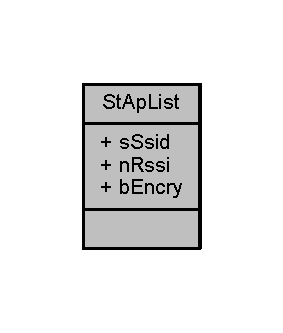
\includegraphics[width=136pt]{struct_st_ap_list__coll__graph}
\end{center}
\end{figure}
\subsection*{데이터 필드}
\begin{DoxyCompactItemize}
\item 
String \mbox{\hyperlink{struct_st_ap_list_a174040ae2c2468aa44f5c18ad915e7a3}{s\+Ssid}}
\item 
signed int \mbox{\hyperlink{struct_st_ap_list_a04d6ede44986822269e924bb50a48369}{n\+Rssi}}
\item 
bool \mbox{\hyperlink{struct_st_ap_list_a3491c9e85ee7dced99ca9b0ff6ea0327}{b\+Encry}}
\end{DoxyCompactItemize}


\subsection{상세한 설명}
주변 검색된 A\+P리스트의 정보를 담는 구조체 (암호화 여부와 수신세기를 포함) 

Wall\+Pad\+Common.\+h 파일의 37 번째 라인에서 정의되었습니다.



\subsection{필드 문서화}
\mbox{\Hypertarget{struct_st_ap_list_a3491c9e85ee7dced99ca9b0ff6ea0327}\label{struct_st_ap_list_a3491c9e85ee7dced99ca9b0ff6ea0327}} 
\index{St\+Ap\+List@{St\+Ap\+List}!b\+Encry@{b\+Encry}}
\index{b\+Encry@{b\+Encry}!St\+Ap\+List@{St\+Ap\+List}}
\subsubsection{\texorpdfstring{b\+Encry}{bEncry}}
{\footnotesize\ttfamily bool b\+Encry}



Wall\+Pad\+Common.\+h 파일의 41 번째 라인에서 정의되었습니다.

\mbox{\Hypertarget{struct_st_ap_list_a04d6ede44986822269e924bb50a48369}\label{struct_st_ap_list_a04d6ede44986822269e924bb50a48369}} 
\index{St\+Ap\+List@{St\+Ap\+List}!n\+Rssi@{n\+Rssi}}
\index{n\+Rssi@{n\+Rssi}!St\+Ap\+List@{St\+Ap\+List}}
\subsubsection{\texorpdfstring{n\+Rssi}{nRssi}}
{\footnotesize\ttfamily signed int n\+Rssi}



Wall\+Pad\+Common.\+h 파일의 40 번째 라인에서 정의되었습니다.

\mbox{\Hypertarget{struct_st_ap_list_a174040ae2c2468aa44f5c18ad915e7a3}\label{struct_st_ap_list_a174040ae2c2468aa44f5c18ad915e7a3}} 
\index{St\+Ap\+List@{St\+Ap\+List}!s\+Ssid@{s\+Ssid}}
\index{s\+Ssid@{s\+Ssid}!St\+Ap\+List@{St\+Ap\+List}}
\subsubsection{\texorpdfstring{s\+Ssid}{sSsid}}
{\footnotesize\ttfamily String s\+Ssid}



Wall\+Pad\+Common.\+h 파일의 39 번째 라인에서 정의되었습니다.



이 구조체에 대한 문서화 페이지는 다음의 파일로부터 생성되었습니다.\+:\begin{DoxyCompactItemize}
\item 
\mbox{\hyperlink{_wall_pad_common_8h}{Wall\+Pad\+Common.\+h}}\end{DoxyCompactItemize}

\hypertarget{struct_st_last_send}{}\section{St\+Last\+Send 구조체 참조}
\label{struct_st_last_send}\index{St\+Last\+Send@{St\+Last\+Send}}


업로드가 너무 자주일어나 과금에 영향을 주므로,~\newline
마지막 업로드의 checksum 과 온도정보를 저장하여, aws 에 업로드 주기를 조절하는 구조체  




{\ttfamily \#include $<$Wall\+Pad\+Common.\+h$>$}



St\+Last\+Send에 대한 협력 다이어그램\+:\nopagebreak
\begin{figure}[H]
\begin{center}
\leavevmode
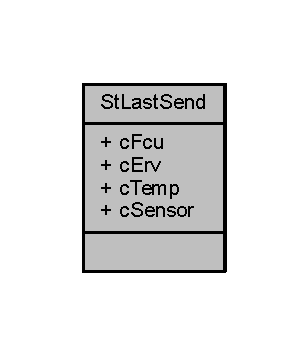
\includegraphics[width=148pt]{struct_st_last_send__coll__graph}
\end{center}
\end{figure}
\subsection*{데이터 필드}
\begin{DoxyCompactItemize}
\item 
char \mbox{\hyperlink{struct_st_last_send_ae99178f09a1a9fed4ba8f4603f165d17}{c\+Fcu}}
\item 
char \mbox{\hyperlink{struct_st_last_send_a47a441ff5eafccfc6171e25c5ea0c311}{c\+Erv}}
\item 
char \mbox{\hyperlink{struct_st_last_send_a7ea4080d1f39154be7d7b1bfd6ff3987}{c\+Temp}}
\item 
char \mbox{\hyperlink{struct_st_last_send_adaef2dbbc191c190520eab895effe14a}{c\+Sensor}}
\end{DoxyCompactItemize}


\subsection{상세한 설명}
업로드가 너무 자주일어나 과금에 영향을 주므로,~\newline
마지막 업로드의 checksum 과 온도정보를 저장하여, aws 에 업로드 주기를 조절하는 구조체 

Wall\+Pad\+Common.\+h 파일의 49 번째 라인에서 정의되었습니다.



\subsection{필드 문서화}
\mbox{\Hypertarget{struct_st_last_send_a47a441ff5eafccfc6171e25c5ea0c311}\label{struct_st_last_send_a47a441ff5eafccfc6171e25c5ea0c311}} 
\index{St\+Last\+Send@{St\+Last\+Send}!c\+Erv@{c\+Erv}}
\index{c\+Erv@{c\+Erv}!St\+Last\+Send@{St\+Last\+Send}}
\subsubsection{\texorpdfstring{c\+Erv}{cErv}}
{\footnotesize\ttfamily char c\+Erv}



Wall\+Pad\+Common.\+h 파일의 52 번째 라인에서 정의되었습니다.

\mbox{\Hypertarget{struct_st_last_send_ae99178f09a1a9fed4ba8f4603f165d17}\label{struct_st_last_send_ae99178f09a1a9fed4ba8f4603f165d17}} 
\index{St\+Last\+Send@{St\+Last\+Send}!c\+Fcu@{c\+Fcu}}
\index{c\+Fcu@{c\+Fcu}!St\+Last\+Send@{St\+Last\+Send}}
\subsubsection{\texorpdfstring{c\+Fcu}{cFcu}}
{\footnotesize\ttfamily char c\+Fcu}



Wall\+Pad\+Common.\+h 파일의 51 번째 라인에서 정의되었습니다.

\mbox{\Hypertarget{struct_st_last_send_adaef2dbbc191c190520eab895effe14a}\label{struct_st_last_send_adaef2dbbc191c190520eab895effe14a}} 
\index{St\+Last\+Send@{St\+Last\+Send}!c\+Sensor@{c\+Sensor}}
\index{c\+Sensor@{c\+Sensor}!St\+Last\+Send@{St\+Last\+Send}}
\subsubsection{\texorpdfstring{c\+Sensor}{cSensor}}
{\footnotesize\ttfamily char c\+Sensor}



Wall\+Pad\+Common.\+h 파일의 54 번째 라인에서 정의되었습니다.

\mbox{\Hypertarget{struct_st_last_send_a7ea4080d1f39154be7d7b1bfd6ff3987}\label{struct_st_last_send_a7ea4080d1f39154be7d7b1bfd6ff3987}} 
\index{St\+Last\+Send@{St\+Last\+Send}!c\+Temp@{c\+Temp}}
\index{c\+Temp@{c\+Temp}!St\+Last\+Send@{St\+Last\+Send}}
\subsubsection{\texorpdfstring{c\+Temp}{cTemp}}
{\footnotesize\ttfamily char c\+Temp}



Wall\+Pad\+Common.\+h 파일의 53 번째 라인에서 정의되었습니다.



이 구조체에 대한 문서화 페이지는 다음의 파일로부터 생성되었습니다.\+:\begin{DoxyCompactItemize}
\item 
\mbox{\hyperlink{_wall_pad_common_8h}{Wall\+Pad\+Common.\+h}}\end{DoxyCompactItemize}

\hypertarget{struct_st_wall_pad}{}\section{St\+Wall\+Pad 구조체 참조}
\label{struct_st_wall_pad}\index{St\+Wall\+Pad@{St\+Wall\+Pad}}


Wall\+Pad의 접속 ssid 와 pw, mode state를 기록하는 구조체  




{\ttfamily \#include $<$Wall\+Pad\+Common.\+h$>$}



St\+Wall\+Pad에 대한 협력 다이어그램\+:\nopagebreak
\begin{figure}[H]
\begin{center}
\leavevmode
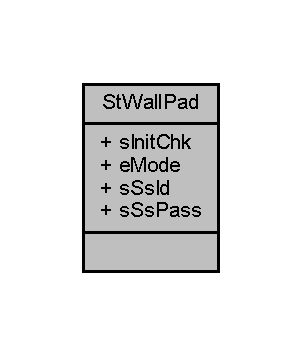
\includegraphics[width=145pt]{struct_st_wall_pad__coll__graph}
\end{center}
\end{figure}
\subsection*{데이터 필드}
\begin{DoxyCompactItemize}
\item 
char \mbox{\hyperlink{struct_st_wall_pad_afa1dc1e2339538ae37ff115251ce1187}{s\+Init\+Chk}} \mbox{[}\mbox{\hyperlink{_wall_pad_common_8h_a633363122e0b4c2005649a1664a2335a}{n\+M\+A\+X\+\_\+\+I\+N\+I\+T\+\_\+\+C\+HK}}\mbox{]}
\item 
\mbox{\hyperlink{_wall_pad_common_8h_a066235770a533eb740dc3fd2494d64da}{e\+M\+O\+DE}} \mbox{\hyperlink{struct_st_wall_pad_a51f947b3c4ad6a33d096bfaf1caedb6e}{e\+Mode}}
\item 
char \mbox{\hyperlink{struct_st_wall_pad_afb1618185a1aecb8c77eff2f1453c24f}{s\+Ss\+Id}} \mbox{[}\mbox{\hyperlink{_wall_pad_common_8h_aa1bfef2ce53d431c709ee094aa02ccb6}{n\+M\+A\+X\+\_\+\+N\+A\+ME}}\mbox{]}
\item 
char \mbox{\hyperlink{struct_st_wall_pad_a8c77e9b61d65201646350d01f8a8d7c0}{s\+Ss\+Pass}} \mbox{[}\mbox{\hyperlink{_wall_pad_common_8h_aa1bfef2ce53d431c709ee094aa02ccb6}{n\+M\+A\+X\+\_\+\+N\+A\+ME}}\mbox{]}
\end{DoxyCompactItemize}


\subsection{상세한 설명}
Wall\+Pad의 접속 ssid 와 pw, mode state를 기록하는 구조체 

Wall\+Pad\+Common.\+h 파일의 20 번째 라인에서 정의되었습니다.



\subsection{필드 문서화}
\mbox{\Hypertarget{struct_st_wall_pad_a51f947b3c4ad6a33d096bfaf1caedb6e}\label{struct_st_wall_pad_a51f947b3c4ad6a33d096bfaf1caedb6e}} 
\index{St\+Wall\+Pad@{St\+Wall\+Pad}!e\+Mode@{e\+Mode}}
\index{e\+Mode@{e\+Mode}!St\+Wall\+Pad@{St\+Wall\+Pad}}
\subsubsection{\texorpdfstring{e\+Mode}{eMode}}
{\footnotesize\ttfamily \mbox{\hyperlink{_wall_pad_common_8h_a066235770a533eb740dc3fd2494d64da}{e\+M\+O\+DE}} e\+Mode}



Wall\+Pad\+Common.\+h 파일의 23 번째 라인에서 정의되었습니다.

\mbox{\Hypertarget{struct_st_wall_pad_afa1dc1e2339538ae37ff115251ce1187}\label{struct_st_wall_pad_afa1dc1e2339538ae37ff115251ce1187}} 
\index{St\+Wall\+Pad@{St\+Wall\+Pad}!s\+Init\+Chk@{s\+Init\+Chk}}
\index{s\+Init\+Chk@{s\+Init\+Chk}!St\+Wall\+Pad@{St\+Wall\+Pad}}
\subsubsection{\texorpdfstring{s\+Init\+Chk}{sInitChk}}
{\footnotesize\ttfamily char s\+Init\+Chk\mbox{[}\mbox{\hyperlink{_wall_pad_common_8h_a633363122e0b4c2005649a1664a2335a}{n\+M\+A\+X\+\_\+\+I\+N\+I\+T\+\_\+\+C\+HK}}\mbox{]}}



Wall\+Pad\+Common.\+h 파일의 22 번째 라인에서 정의되었습니다.

\mbox{\Hypertarget{struct_st_wall_pad_afb1618185a1aecb8c77eff2f1453c24f}\label{struct_st_wall_pad_afb1618185a1aecb8c77eff2f1453c24f}} 
\index{St\+Wall\+Pad@{St\+Wall\+Pad}!s\+Ss\+Id@{s\+Ss\+Id}}
\index{s\+Ss\+Id@{s\+Ss\+Id}!St\+Wall\+Pad@{St\+Wall\+Pad}}
\subsubsection{\texorpdfstring{s\+Ss\+Id}{sSsId}}
{\footnotesize\ttfamily char s\+Ss\+Id\mbox{[}\mbox{\hyperlink{_wall_pad_common_8h_aa1bfef2ce53d431c709ee094aa02ccb6}{n\+M\+A\+X\+\_\+\+N\+A\+ME}}\mbox{]}}



Wall\+Pad\+Common.\+h 파일의 24 번째 라인에서 정의되었습니다.

\mbox{\Hypertarget{struct_st_wall_pad_a8c77e9b61d65201646350d01f8a8d7c0}\label{struct_st_wall_pad_a8c77e9b61d65201646350d01f8a8d7c0}} 
\index{St\+Wall\+Pad@{St\+Wall\+Pad}!s\+Ss\+Pass@{s\+Ss\+Pass}}
\index{s\+Ss\+Pass@{s\+Ss\+Pass}!St\+Wall\+Pad@{St\+Wall\+Pad}}
\subsubsection{\texorpdfstring{s\+Ss\+Pass}{sSsPass}}
{\footnotesize\ttfamily char s\+Ss\+Pass\mbox{[}\mbox{\hyperlink{_wall_pad_common_8h_aa1bfef2ce53d431c709ee094aa02ccb6}{n\+M\+A\+X\+\_\+\+N\+A\+ME}}\mbox{]}}



Wall\+Pad\+Common.\+h 파일의 25 번째 라인에서 정의되었습니다.



이 구조체에 대한 문서화 페이지는 다음의 파일로부터 생성되었습니다.\+:\begin{DoxyCompactItemize}
\item 
\mbox{\hyperlink{_wall_pad_common_8h}{Wall\+Pad\+Common.\+h}}\end{DoxyCompactItemize}

\chapter{파일 문서화}
\hypertarget{sl__uart__task_8c}{}\section{sl\+\_\+uart\+\_\+task.\+c 파일 참조}
\label{sl__uart__task_8c}\index{sl\+\_\+uart\+\_\+task.\+c@{sl\+\_\+uart\+\_\+task.\+c}}
{\ttfamily \#include $<$Arduino.\+h$>$}\newline
{\ttfamily \#include $<$Stream.\+h$>$}\newline
{\ttfamily \#include $<$E\+E\+P\+R\+O\+M.\+h$>$}\newline
{\ttfamily \#include $<$E\+S\+P8266\+Wi\+Fi.\+h$>$}\newline
{\ttfamily \#include $<$E\+S\+P8266\+Wi\+Fi\+Multi.\+h$>$}\newline
{\ttfamily \#include \char`\"{}sha256.\+h\char`\"{}}\newline
{\ttfamily \#include \char`\"{}Utils.\+h\char`\"{}}\newline
{\ttfamily \#include $<$Hash.\+h$>$}\newline
{\ttfamily \#include $<$Web\+Sockets\+Client.\+h$>$}\newline
{\ttfamily \#include $<$Pub\+Sub\+Client.\+h$>$}\newline
{\ttfamily \#include \char`\"{}Wall\+Pad\+Common.\+h\char`\"{}}\newline
{\ttfamily \#include \char`\"{}Client.\+h\char`\"{}}\newline
{\ttfamily \#include \char`\"{}A\+W\+S\+Web\+Socket\+Client.\+h\char`\"{}}\newline
{\ttfamily \#include \char`\"{}Circular\+Byte\+Buffer.\+h\char`\"{}}\newline
{\ttfamily \#include $<$stdarg.\+h$>$}\newline
{\ttfamily \#include $<$os\+\_\+type.\+h$>$}\newline
{\ttfamily \#include \char`\"{}user\+\_\+interface.\+h\char`\"{}}\newline
{\ttfamily \#include $<$osapi.\+h$>$}\newline
sl\+\_\+uart\+\_\+task.\+c에 대한 include 의존 그래프\nopagebreak
\begin{figure}[H]
\begin{center}
\leavevmode
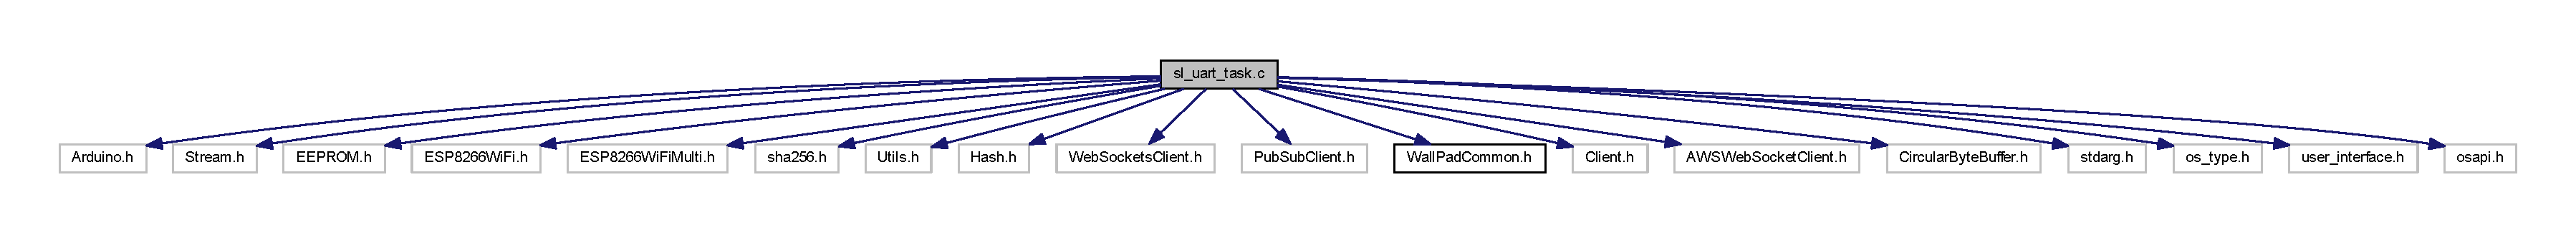
\includegraphics[width=350pt]{sl__uart__task_8c__incl}
\end{center}
\end{figure}
\subsection*{매크로}
\begin{DoxyCompactItemize}
\item 
\#define \mbox{\hyperlink{sl__uart__task_8c_a161f66c89721d6e10e0f626e305c6013}{Wallpad\+Serial}}~Serial
\item 
\#define \mbox{\hyperlink{sl__uart__task_8c_a0dc0281c6f27e62a5cb21cde5288a9a5}{Debug\+Serial}}~Serial1
\item 
\#define \mbox{\hyperlink{sl__uart__task_8c_a5bdd6772c246436bb14377095de79b31}{U\+A\+R\+T\+\_\+\+R\+X\+\_\+\+B\+U\+F\+F\+E\+R\+\_\+\+S\+I\+ZE}}~1024
\item 
\#define \mbox{\hyperlink{sl__uart__task_8c_aca8e8e20d2136c68476203baa1ee3029}{U\+A\+R\+T\+\_\+\+R\+X\+\_\+\+T\+A\+S\+K\+\_\+\+P\+R\+I\+O\+R\+I\+TY}}~1
\item 
\#define \mbox{\hyperlink{sl__uart__task_8c_a57dcc29bb266003c63803b06ea25b26d}{U\+A\+R\+T\+\_\+\+T\+A\+S\+K\+\_\+\+P\+R\+I\+O\+R\+I\+TY}}~0
\item 
\#define \mbox{\hyperlink{sl__uart__task_8c_a6a9f5253345bffef8276cc5070177572}{U\+A\+R\+T\+\_\+\+R\+X\+\_\+\+Q\+U\+E\+U\+E\+\_\+\+S\+I\+ZE}}~8
\end{DoxyCompactItemize}
\subsection*{함수}
\begin{DoxyCompactItemize}
\item 
int \mbox{\hyperlink{sl__uart__task_8c_a38f7f9361dece3c36092a307f845f0a6}{checksum}} (char $\ast$data)
\begin{DoxyCompactList}\small\item\em 오류 확인 함수 \end{DoxyCompactList}\item 
void \mbox{\hyperlink{sl__uart__task_8c_a20ce1fcbc3f39da9ceaf09dbd5ca5ef8}{responsecmd}} (char $\ast$readcmd)
\begin{DoxyCompactList}\small\item\em 응답 데이터 형식지정 함수 \end{DoxyCompactList}\item 
A\+W\+S\+Web\+Socket\+Client \mbox{\hyperlink{sl__uart__task_8c_af273a6e233df1fa0ded638e07843b468}{aws\+W\+Sclient}} (1024)
\item 
Pub\+Sub\+Client \mbox{\hyperlink{sl__uart__task_8c_aed38f3e7ee0565ea6703f91a12983f54}{client}} (\mbox{\hyperlink{sl__uart__task_8c_af273a6e233df1fa0ded638e07843b468}{aws\+W\+Sclient}})
\item 
char $\ast$ \mbox{\hyperlink{sl__uart__task_8c_a0db6cddb7699ddbce4aa6f489d7d7879}{generate\+Client\+ID}} ()
\begin{DoxyCompactList}\small\item\em 클라이언트 ID 자동생성 함수 \end{DoxyCompactList}\item 
bool \mbox{\hyperlink{sl__uart__task_8c_aa0a57e883c6c9fc19e62a609d967be9c}{connect}} ()
\begin{DoxyCompactList}\small\item\em websocket \& M\+Q\+TT 접속 함수 \end{DoxyCompactList}\item 
void \mbox{\hyperlink{sl__uart__task_8c_a0bccd94c4239c019c480e507cb6159ee}{subscribe}} ()
\begin{DoxyCompactList}\small\item\em M\+Q\+TT subscribe 함수 \end{DoxyCompactList}\item 
void \mbox{\hyperlink{sl__uart__task_8c_a8a2d61a985df99709d3d8c5ef7d46605}{send\+Aws\+Msg}} (char $\ast$readcmd, bool appstate)
\begin{DoxyCompactList}\small\item\em publishing 함수 \end{DoxyCompactList}\item 
void \mbox{\hyperlink{sl__uart__task_8c_ac3a129f66dc859e2b7279565f4e1de78}{callback}} (char $\ast$topic, byte $\ast$payload, unsigned int length)
\begin{DoxyCompactList}\small\item\em callback 함수 \end{DoxyCompactList}\item 
void \mbox{\hyperlink{sl__uart__task_8c_a93049dd8aee54bb4e745e526542c36f7}{Temp\+\_\+\+Run\+\_\+\+U\+A\+R\+T\+\_\+\+R\+X\+\_\+\+Task}} (void $\ast$)
\begin{DoxyCompactList}\small\item\em task 메세지를 보내는 함수 \end{DoxyCompactList}\item 
void \mbox{\hyperlink{sl__uart__task_8c_aac99a2341cbcfcbd24f7aba50e2ff771}{send\+Aws\+Msg}} (char $\ast$readcmd)
\item 
void \mbox{\hyperlink{sl__uart__task_8c_a35bd387bc89edc5110da50f77d737813}{U\+A\+R\+T\+\_\+\+R\+X\+\_\+\+T\+A\+S\+K\+\_\+\+Handler}} (os\+\_\+event\+\_\+t $\ast$)
\begin{DoxyCompactList}\small\item\em U\+A\+R\+T\+\_\+\+R\+X\+\_\+\+T\+A\+S\+K\+\_\+\+Handler함수 (트랩) \end{DoxyCompactList}\item 
void \mbox{\hyperlink{sl__uart__task_8c_aed00320e0a0898df9eed984a3ced0ad8}{Init\+Eeprom}} (void)
\begin{DoxyCompactList}\small\item\em E\+E\+P\+R\+OM 초기화 함수 \end{DoxyCompactList}\item 
void \mbox{\hyperlink{sl__uart__task_8c_a77d6a883c5cf0c92dcc225685249e38e}{Store\+Eeprom}} (void)
\begin{DoxyCompactList}\small\item\em E\+E\+P\+R\+OM 쓰기 함수 \end{DoxyCompactList}\item 
void \mbox{\hyperlink{sl__uart__task_8c_a707a658761cc8b67188a0eb67ba9103e}{Load\+Eeprom}} (void)
\begin{DoxyCompactList}\small\item\em E\+E\+P\+R\+OM 읽기 함수 \end{DoxyCompactList}\item 
void \mbox{\hyperlink{sl__uart__task_8c_ac4dd7f628ac36ff312d47a898d0573d6}{Check\+Eeprom}} (void)
\begin{DoxyCompactList}\small\item\em E\+E\+P\+R\+OM 체크 함수 \end{DoxyCompactList}\item 
I\+P\+Address \mbox{\hyperlink{sl__uart__task_8c_a70c83cd124803780a6e042045ec2d029}{local\+\_\+\+IP}} (192, 168, 1, 1)
\item 
I\+P\+Address \mbox{\hyperlink{sl__uart__task_8c_a140be8626580a0cb94729a6615877d40}{gateway}} (192, 168, 1, 1)
\item 
I\+P\+Address \mbox{\hyperlink{sl__uart__task_8c_a89cf134ada28d8ce0192d9fcbc83614a}{subnet}} (255, 255, 255, 0)
\item 
Wi\+Fi\+Server \mbox{\hyperlink{sl__uart__task_8c_a5042d50338e981034cfb61c6067ab043}{server}} (30300)
\item 
int \mbox{\hyperlink{sl__uart__task_8c_a4476697452689e3561ad2909c9047f4a}{Find\+Ap}} (bool ap)
\begin{DoxyCompactList}\small\item\em wifi 신호 탐색 함수 \end{DoxyCompactList}\item 
void \mbox{\hyperlink{sl__uart__task_8c_ac923d0bf25ed513586077a218b54f4e5}{Apmode}} ()
\begin{DoxyCompactList}\small\item\em wifi 서비스 함수 \end{DoxyCompactList}\item 
void \mbox{\hyperlink{sl__uart__task_8c_a5b6b4e47c7e5a413015c702d9825734f}{Connect}} ()
\begin{DoxyCompactList}\small\item\em wifi \& aws 접속 함수 \end{DoxyCompactList}\item 
void \mbox{\hyperlink{sl__uart__task_8c_a4fc01d736fe50cf5b977f755b675f11d}{setup}} ()
\begin{DoxyCompactList}\small\item\em task 설정 함수 \end{DoxyCompactList}\item 
void \mbox{\hyperlink{sl__uart__task_8c_afe461d27b9c48d5921c00d521181f12f}{loop}} ()
\begin{DoxyCompactList}\small\item\em e\+Mode 함수 \end{DoxyCompactList}\end{DoxyCompactItemize}
\subsection*{변수}
\begin{DoxyCompactItemize}
\item 
static \mbox{\hyperlink{_wall_pad_common_8h_afc78910c4749fa1230e1149115f9d70a}{Wall\+Pad}} \mbox{\hyperlink{sl__uart__task_8c_a45bb259cfa999c850530718ccac5609b}{g\+\_\+\+Wall\+Pad}}
\item 
static char \mbox{\hyperlink{sl__uart__task_8c_aae63324171e03f0c269b3efa7916690c}{g\+\_\+\+Device\+Name}} \mbox{[}\mbox{\hyperlink{_wall_pad_common_8h_aa1bfef2ce53d431c709ee094aa02ccb6}{n\+M\+A\+X\+\_\+\+N\+A\+ME}}\mbox{]} = \char`\"{}S\+L\+T\+\_\+\+F\+C\+UR-\/W\+T\+E\+S\+T2\char`\"{}
\begin{DoxyCompactList}\small\item\em 장비 이름을 저장하는 변수 \end{DoxyCompactList}\item 
static char \mbox{\hyperlink{sl__uart__task_8c_a888896fba8b48ebf2107d770e642e37f}{g\+\_\+s\+Init\+Title}} \mbox{[}\mbox{\hyperlink{_wall_pad_common_8h_a633363122e0b4c2005649a1664a2335a}{n\+M\+A\+X\+\_\+\+I\+N\+I\+T\+\_\+\+C\+HK}}\mbox{]} = \char`\"{}S\+L\+Tech. Wall\+Pad. V2.\+1(2018.\+02.\+13)\char`\"{}
\begin{DoxyCompactList}\small\item\em 장비 버전 정보를 담는 초기화 체크 변수 \end{DoxyCompactList}\item 
static char \mbox{\hyperlink{sl__uart__task_8c_aa5d0ec846e4a5c3218b26ac91b89c137}{g\+\_\+s\+Init\+Ssid}} \mbox{[}\mbox{\hyperlink{_wall_pad_common_8h_aa1bfef2ce53d431c709ee094aa02ccb6}{n\+M\+A\+X\+\_\+\+N\+A\+ME}}\mbox{]} = \char`\"{}\char`\"{}
\begin{DoxyCompactList}\small\item\em 와이파이 접속 정보중 S\+S\+I\+D를 담는 변수 \end{DoxyCompactList}\item 
static char \mbox{\hyperlink{sl__uart__task_8c_a1bdc597aadbd6a0b8f8ddfdc4aee425e}{g\+\_\+s\+Init\+Sspass}} \mbox{[}\mbox{\hyperlink{_wall_pad_common_8h_aa1bfef2ce53d431c709ee094aa02ccb6}{n\+M\+A\+X\+\_\+\+N\+A\+ME}}\mbox{]} = \char`\"{}\char`\"{}
\begin{DoxyCompactList}\small\item\em 와이파이 접속 정보중 비밀번호를 담는 변수 \end{DoxyCompactList}\item 
static \mbox{\hyperlink{_wall_pad_common_8h_aa98442922a779292a101450d76255385}{Ap\+List}} \mbox{\hyperlink{sl__uart__task_8c_ab172c51f9996185c00e7eedc1f28b24a}{g\+\_\+\+Ap\+List}} \mbox{[}\mbox{\hyperlink{_wall_pad_common_8h_ac370fa01d5773341bbcc501c01c11d1e}{n\+M\+A\+X\+\_\+\+S\+E\+A\+R\+C\+H\+\_\+\+AP}}\mbox{]}
\item 
static \mbox{\hyperlink{_wall_pad_common_8h_ad2d28182118d0dc42728639623d2dc40}{p\+Ap\+List}} \mbox{\hyperlink{sl__uart__task_8c_a41db1cc0774aca1f9cbe536a9c5a518e}{g\+\_\+p\+Ap\+List}} \mbox{[}\mbox{\hyperlink{_wall_pad_common_8h_ac370fa01d5773341bbcc501c01c11d1e}{n\+M\+A\+X\+\_\+\+S\+E\+A\+R\+C\+H\+\_\+\+AP}}\mbox{]}
\item 
static int \mbox{\hyperlink{sl__uart__task_8c_a360ac0bcfdbb88764f1535bce0361cea}{g\+\_\+n\+Max\+Ap}}
\begin{DoxyCompactList}\small\item\em 주변 A\+P리스트를 저장하는 변수 \end{DoxyCompactList}\item 
static \mbox{\hyperlink{_wall_pad_common_8h_a78ff28de5f4a28ca30a16c6e0f7b0d35}{Last\+Send}} \mbox{\hyperlink{sl__uart__task_8c_a9ee5ac74e0a6f3ba41e7bbcd03c316f4}{g\+\_\+\+Last\+Send}}
\item 
char \mbox{\hyperlink{sl__uart__task_8c_a073128b0e46bc8edcc1b5ea52715bddd}{g\+\_\+cmd}} \mbox{[}8\mbox{]} = \{0x00,\}
\begin{DoxyCompactList}\small\item\em mqtt 수신 정보를 기록하는 글로벌 변수 \end{DoxyCompactList}\item 
int \mbox{\hyperlink{sl__uart__task_8c_a9eaf86bfd30962df9aff407bd4840336}{g\+\_\+msg\+Send}} = 0
\begin{DoxyCompactList}\small\item\em mqtt 수신 트리거 변수 \end{DoxyCompactList}\item 
bool \mbox{\hyperlink{sl__uart__task_8c_aa557e6b05fc785e99ccfc9b09bc79bc5}{g\+\_\+b\+Connecting}} = false
\begin{DoxyCompactList}\small\item\em 와이파이 연결 정보를 관리하기 위한 글로벌 변수 \end{DoxyCompactList}\item 
bool \mbox{\hyperlink{sl__uart__task_8c_a06be4e59ee6e13a5f54dba4c3f014ec5}{g\+\_\+b\+Appctl}} = false
\item 
char \mbox{\hyperlink{sl__uart__task_8c_ac46d88a622b98a0106aaa722ef71d91e}{wifi\+\_\+ssid}} \mbox{[}$\,$\mbox{]} = \char`\"{}godjaehyeok\char`\"{}
\item 
char \mbox{\hyperlink{sl__uart__task_8c_aa7d10360d34ad6eca06d1803b3d1c3ef}{wifi\+\_\+password}} \mbox{[}$\,$\mbox{]} = \char`\"{}gjwogur123\char`\"{}
\item 
char \mbox{\hyperlink{sl__uart__task_8c_a0977a0891557a2a5f83b635e5eb3443e}{aws\+\_\+endpoint}} \mbox{[}$\,$\mbox{]} = \char`\"{}a2q36qubve1ukk.\+iot.\+ap-\/northeast-\/2.amazonaws.\+com\char`\"{}
\item 
char \mbox{\hyperlink{sl__uart__task_8c_a45bf1e976b70d29f3c109c37a3b01b88}{aws\+\_\+key}} \mbox{[}$\,$\mbox{]} = \char`\"{}A\+K\+I\+A\+J\+A4\+X53\+V\+A\+F\+T\+G\+E\+D\+Q3Q\char`\"{}
\item 
char \mbox{\hyperlink{sl__uart__task_8c_a1297e4248f6e6a429598f485126a19ce}{aws\+\_\+secret}} \mbox{[}$\,$\mbox{]} = \char`\"{}mxmno\+Wt+exqgfce5\+Hv+DE/h5m\+Oeo\+Xd\+A\+Bf\+M\+Jq\+Eg\+Rg\char`\"{}
\item 
char \mbox{\hyperlink{sl__uart__task_8c_a3c3e0be700ab12b748d8c833ee2255a1}{aws\+\_\+region}} \mbox{[}$\,$\mbox{]} = \char`\"{}ap-\/northeast-\/2\char`\"{}
\item 
const char $\ast$ \mbox{\hyperlink{sl__uart__task_8c_af0a4f1814f6df77902506d568db1b886}{aws\+\_\+topic\+\_\+update}} = \char`\"{}\$aws/things/test2/shadow/update\char`\"{}
\item 
const char $\ast$ \mbox{\hyperlink{sl__uart__task_8c_a1bffe679a4beca9eb4d24e8a6d72ec8a}{aws\+\_\+topic}} = \char`\"{}\$aws/things/test2/shadow/update/accepted\char`\"{}
\item 
int \mbox{\hyperlink{sl__uart__task_8c_a63c89c04d1feae07ca35558055155ffb}{port}} = 443
\item 
long \mbox{\hyperlink{sl__uart__task_8c_ad268c14b4a9086cd1b67ca1d86f417d5}{connection}} = 0
\item 
const int \mbox{\hyperlink{sl__uart__task_8c_ae009fdfed6fa68c3a5eefd9dd3c70776}{max\+M\+Q\+T\+Tpackage\+Size}} = 512
\item 
const int \mbox{\hyperlink{sl__uart__task_8c_a0535d4bdc7c07ab9b44c5d1d1c4c547b}{max\+M\+Q\+T\+T\+Message\+Handlers}} = 1
\item 
E\+S\+P8266\+Wi\+Fi\+Multi \mbox{\hyperlink{sl__uart__task_8c_a17dc5624a7578d8675ef9fed1b260754}{Wi\+Fi\+Multi}}
\item 
uint8\+\_\+t \mbox{\hyperlink{sl__uart__task_8c_a67a3128df98beb6b898eda59b409afe3}{U\+A\+R\+T\+\_\+\+R\+X\+\_\+\+B\+U\+F\+F\+ER}} \mbox{[}\mbox{\hyperlink{sl__uart__task_8c_a5bdd6772c246436bb14377095de79b31}{U\+A\+R\+T\+\_\+\+R\+X\+\_\+\+B\+U\+F\+F\+E\+R\+\_\+\+S\+I\+ZE}}\mbox{]}
\item 
long int \mbox{\hyperlink{sl__uart__task_8c_a22008b8070a494b741d2caed0596e86d}{U\+A\+R\+T\+\_\+\+R\+X\+\_\+\+R\+E\+C\+E\+I\+V\+E\+\_\+\+C\+O\+U\+NT}} = 0
\item 
static os\+\_\+timer\+\_\+t \mbox{\hyperlink{sl__uart__task_8c_aaab2b2dd61c91cddbaa9e130d26d5dce}{U\+A\+R\+T\+\_\+\+R\+X\+\_\+\+T\+A\+S\+K\+\_\+\+Timer}}
\item 
static os\+\_\+timer\+\_\+t \mbox{\hyperlink{sl__uart__task_8c_ad1c65a91fad108d5f581b43defe1007a}{U\+A\+R\+T\+\_\+\+T\+A\+S\+K\+\_\+\+Timer}}
\item 
static os\+\_\+event\+\_\+t \mbox{\hyperlink{sl__uart__task_8c_aa67c702a9e31bd1b512f4ac8b152c65d}{U\+A\+R\+T\+\_\+\+R\+X\+\_\+\+Q\+U\+E\+UE}} \mbox{[}\mbox{\hyperlink{sl__uart__task_8c_a6a9f5253345bffef8276cc5070177572}{U\+A\+R\+T\+\_\+\+R\+X\+\_\+\+Q\+U\+E\+U\+E\+\_\+\+S\+I\+ZE}}\mbox{]}
\item 
long int \mbox{\hyperlink{sl__uart__task_8c_a36baaeb855e27ca3d67e6e3e0230e974}{U\+A\+R\+T\+\_\+\+R\+X\+\_\+\+C\+Y\+C\+L\+E\+\_\+\+I\+N\+\_\+\+MS}} = 100
\item 
Wi\+Fi\+Client \mbox{\hyperlink{sl__uart__task_8c_abbb6f0d4140565a3f0e833a4dc0ca10e}{tcpclient}}
\end{DoxyCompactItemize}


\subsection{매크로 문서화}
\mbox{\Hypertarget{sl__uart__task_8c_a0dc0281c6f27e62a5cb21cde5288a9a5}\label{sl__uart__task_8c_a0dc0281c6f27e62a5cb21cde5288a9a5}} 
\index{sl\+\_\+uart\+\_\+task.\+c@{sl\+\_\+uart\+\_\+task.\+c}!Debug\+Serial@{Debug\+Serial}}
\index{Debug\+Serial@{Debug\+Serial}!sl\+\_\+uart\+\_\+task.\+c@{sl\+\_\+uart\+\_\+task.\+c}}
\subsubsection{\texorpdfstring{Debug\+Serial}{DebugSerial}}
{\footnotesize\ttfamily \#define Debug\+Serial~Serial1}



sl\+\_\+uart\+\_\+task.\+c 파일의 72 번째 라인에서 정의되었습니다.

\mbox{\Hypertarget{sl__uart__task_8c_a5bdd6772c246436bb14377095de79b31}\label{sl__uart__task_8c_a5bdd6772c246436bb14377095de79b31}} 
\index{sl\+\_\+uart\+\_\+task.\+c@{sl\+\_\+uart\+\_\+task.\+c}!U\+A\+R\+T\+\_\+\+R\+X\+\_\+\+B\+U\+F\+F\+E\+R\+\_\+\+S\+I\+ZE@{U\+A\+R\+T\+\_\+\+R\+X\+\_\+\+B\+U\+F\+F\+E\+R\+\_\+\+S\+I\+ZE}}
\index{U\+A\+R\+T\+\_\+\+R\+X\+\_\+\+B\+U\+F\+F\+E\+R\+\_\+\+S\+I\+ZE@{U\+A\+R\+T\+\_\+\+R\+X\+\_\+\+B\+U\+F\+F\+E\+R\+\_\+\+S\+I\+ZE}!sl\+\_\+uart\+\_\+task.\+c@{sl\+\_\+uart\+\_\+task.\+c}}
\subsubsection{\texorpdfstring{U\+A\+R\+T\+\_\+\+R\+X\+\_\+\+B\+U\+F\+F\+E\+R\+\_\+\+S\+I\+ZE}{UART\_RX\_BUFFER\_SIZE}}
{\footnotesize\ttfamily \#define U\+A\+R\+T\+\_\+\+R\+X\+\_\+\+B\+U\+F\+F\+E\+R\+\_\+\+S\+I\+ZE~1024}



sl\+\_\+uart\+\_\+task.\+c 파일의 487 번째 라인에서 정의되었습니다.

\mbox{\Hypertarget{sl__uart__task_8c_a6a9f5253345bffef8276cc5070177572}\label{sl__uart__task_8c_a6a9f5253345bffef8276cc5070177572}} 
\index{sl\+\_\+uart\+\_\+task.\+c@{sl\+\_\+uart\+\_\+task.\+c}!U\+A\+R\+T\+\_\+\+R\+X\+\_\+\+Q\+U\+E\+U\+E\+\_\+\+S\+I\+ZE@{U\+A\+R\+T\+\_\+\+R\+X\+\_\+\+Q\+U\+E\+U\+E\+\_\+\+S\+I\+ZE}}
\index{U\+A\+R\+T\+\_\+\+R\+X\+\_\+\+Q\+U\+E\+U\+E\+\_\+\+S\+I\+ZE@{U\+A\+R\+T\+\_\+\+R\+X\+\_\+\+Q\+U\+E\+U\+E\+\_\+\+S\+I\+ZE}!sl\+\_\+uart\+\_\+task.\+c@{sl\+\_\+uart\+\_\+task.\+c}}
\subsubsection{\texorpdfstring{U\+A\+R\+T\+\_\+\+R\+X\+\_\+\+Q\+U\+E\+U\+E\+\_\+\+S\+I\+ZE}{UART\_RX\_QUEUE\_SIZE}}
{\footnotesize\ttfamily \#define U\+A\+R\+T\+\_\+\+R\+X\+\_\+\+Q\+U\+E\+U\+E\+\_\+\+S\+I\+ZE~8}



sl\+\_\+uart\+\_\+task.\+c 파일의 494 번째 라인에서 정의되었습니다.

\mbox{\Hypertarget{sl__uart__task_8c_aca8e8e20d2136c68476203baa1ee3029}\label{sl__uart__task_8c_aca8e8e20d2136c68476203baa1ee3029}} 
\index{sl\+\_\+uart\+\_\+task.\+c@{sl\+\_\+uart\+\_\+task.\+c}!U\+A\+R\+T\+\_\+\+R\+X\+\_\+\+T\+A\+S\+K\+\_\+\+P\+R\+I\+O\+R\+I\+TY@{U\+A\+R\+T\+\_\+\+R\+X\+\_\+\+T\+A\+S\+K\+\_\+\+P\+R\+I\+O\+R\+I\+TY}}
\index{U\+A\+R\+T\+\_\+\+R\+X\+\_\+\+T\+A\+S\+K\+\_\+\+P\+R\+I\+O\+R\+I\+TY@{U\+A\+R\+T\+\_\+\+R\+X\+\_\+\+T\+A\+S\+K\+\_\+\+P\+R\+I\+O\+R\+I\+TY}!sl\+\_\+uart\+\_\+task.\+c@{sl\+\_\+uart\+\_\+task.\+c}}
\subsubsection{\texorpdfstring{U\+A\+R\+T\+\_\+\+R\+X\+\_\+\+T\+A\+S\+K\+\_\+\+P\+R\+I\+O\+R\+I\+TY}{UART\_RX\_TASK\_PRIORITY}}
{\footnotesize\ttfamily \#define U\+A\+R\+T\+\_\+\+R\+X\+\_\+\+T\+A\+S\+K\+\_\+\+P\+R\+I\+O\+R\+I\+TY~1}



sl\+\_\+uart\+\_\+task.\+c 파일의 491 번째 라인에서 정의되었습니다.

\mbox{\Hypertarget{sl__uart__task_8c_a57dcc29bb266003c63803b06ea25b26d}\label{sl__uart__task_8c_a57dcc29bb266003c63803b06ea25b26d}} 
\index{sl\+\_\+uart\+\_\+task.\+c@{sl\+\_\+uart\+\_\+task.\+c}!U\+A\+R\+T\+\_\+\+T\+A\+S\+K\+\_\+\+P\+R\+I\+O\+R\+I\+TY@{U\+A\+R\+T\+\_\+\+T\+A\+S\+K\+\_\+\+P\+R\+I\+O\+R\+I\+TY}}
\index{U\+A\+R\+T\+\_\+\+T\+A\+S\+K\+\_\+\+P\+R\+I\+O\+R\+I\+TY@{U\+A\+R\+T\+\_\+\+T\+A\+S\+K\+\_\+\+P\+R\+I\+O\+R\+I\+TY}!sl\+\_\+uart\+\_\+task.\+c@{sl\+\_\+uart\+\_\+task.\+c}}
\subsubsection{\texorpdfstring{U\+A\+R\+T\+\_\+\+T\+A\+S\+K\+\_\+\+P\+R\+I\+O\+R\+I\+TY}{UART\_TASK\_PRIORITY}}
{\footnotesize\ttfamily \#define U\+A\+R\+T\+\_\+\+T\+A\+S\+K\+\_\+\+P\+R\+I\+O\+R\+I\+TY~0}



sl\+\_\+uart\+\_\+task.\+c 파일의 492 번째 라인에서 정의되었습니다.

\mbox{\Hypertarget{sl__uart__task_8c_a161f66c89721d6e10e0f626e305c6013}\label{sl__uart__task_8c_a161f66c89721d6e10e0f626e305c6013}} 
\index{sl\+\_\+uart\+\_\+task.\+c@{sl\+\_\+uart\+\_\+task.\+c}!Wallpad\+Serial@{Wallpad\+Serial}}
\index{Wallpad\+Serial@{Wallpad\+Serial}!sl\+\_\+uart\+\_\+task.\+c@{sl\+\_\+uart\+\_\+task.\+c}}
\subsubsection{\texorpdfstring{Wallpad\+Serial}{WallpadSerial}}
{\footnotesize\ttfamily \#define Wallpad\+Serial~Serial}



sl\+\_\+uart\+\_\+task.\+c 파일의 71 번째 라인에서 정의되었습니다.



\subsection{함수 문서화}
\mbox{\Hypertarget{sl__uart__task_8c_ac923d0bf25ed513586077a218b54f4e5}\label{sl__uart__task_8c_ac923d0bf25ed513586077a218b54f4e5}} 
\index{sl\+\_\+uart\+\_\+task.\+c@{sl\+\_\+uart\+\_\+task.\+c}!Apmode@{Apmode}}
\index{Apmode@{Apmode}!sl\+\_\+uart\+\_\+task.\+c@{sl\+\_\+uart\+\_\+task.\+c}}
\subsubsection{\texorpdfstring{Apmode()}{Apmode()}}
{\footnotesize\ttfamily void Apmode (\begin{DoxyParamCaption}{ }\end{DoxyParamCaption})}



wifi 서비스 함수 

wifi 서버로 역할을 하고 접속된 클라이언트의 정보에 따라 클라이언트에게 필요한 메세지를 보내준다 \begin{DoxySeeAlso}{참고}
이 함수의 코드분석 내용
\begin{DoxyEnumerate}
\item wifi가 접속되어 있는지 판단하고 연결되어있으면 연결을 끊는다~\newline

\item AP mode에 대한 ip가 설정이 안되었다면, mode를 A\+P\+\_\+\+S\+T\+A로 바꾸고, IP, \mbox{\hyperlink{sl__uart__task_8c_a140be8626580a0cb94729a6615877d40}{gateway}}, subnet를 설정 후~\newline
 장비 이름 설정하고 wifi서버를 실행한다~\newline

\item 클라이언트가 서버와 연결 할 수 없다면, 서버에서 이용할 수 있도록 허용해준다~\newline

\item 서버와 클라이언트가 연결 되었다면, 클라이언트의 데이터의 양을 확인한다~\newline

\item 클라이언트 정보 18byte를 버퍼에 저장한다~\newline

\item 버퍼에 내용 중에 \char`\"{}\+S\+P\+H\+I\+O\+T0010\char`\"{}이 있는지 확인한다~\newline

\item 관련 문자열이 있다면, 버퍼의 내용 중 일부를 이용하여 경우따라 방침을 만든다~\newline

\item 101 \+: find\+Ap 함수를 호출한다
\item 101 \+: global 변수(int) \mbox{\hyperlink{sl__uart__task_8c_a360ac0bcfdbb88764f1535bce0361cea}{g\+\_\+n\+Max\+Ap}} 수가 10이상 경우, 10으로 고정하여 10$\ast$32의 값을 변수(int) bodysize에 대입한다~\newline

\item 101 \+: 버퍼에 \char`\"{}\+S\+P\+H\+I\+O\+T0010\char`\"{}문자열과 201, 정해진 사이즈를 입력한다~\newline

\item 101 \+: 클라이언트에게 버퍼를 내용을 전달한다~\newline

\item 101 \+: (global 변수(int) \mbox{\hyperlink{sl__uart__task_8c_a360ac0bcfdbb88764f1535bce0361cea}{g\+\_\+n\+Max\+Ap}} 만큼 반복 $<$단, 10이상 도달 시 이 조건문을 나오게된다$>$)~\newline
 global 구조체배열 \mbox{\hyperlink{sl__uart__task_8c_ab172c51f9996185c00e7eedc1f28b24a}{g\+\_\+\+Ap\+List}} s\+Ssid를 ap버퍼에 저장하고, 클라이언트에게 전달한다~\newline

\item 101 \+: 32 -\/ s\+Ssid길이 뺀 숫자만큼 반복하여 클라이언트에게 \textquotesingle{} \textquotesingle{}을 보낸다~\newline

\item 102 \+: 클라이언트 정보 128byte를 힙 버퍼에 저장한다~\newline

\item 102 \+: 힙 버퍼를 \char`\"{} \char`\"{}문자열로 첫 분류에서 나온 문자열을 global 배열\mbox{[}char\mbox{]} g\+\_\+s\+Init\+Ssid에 대입한다~\newline

\item 102 \+: 힙 버퍼를 \char`\"{} \char`\"{}문자열로 그다음 분류에서 나온 문자열을 global 배열\mbox{[}char\mbox{]} g\+\_\+s\+Init\+Sspass에 대입한다~\newline

\item 102 \+: global 구조체 g\+\_\+\+Wall\+Pad의 e\+Mode를 e\+M\+O\+D\+E\+\_\+\+C\+O\+N\+N\+E\+C\+T으로 변환한다~\newline

\item 104 \+: bodysize를 4로 대입하고, 버퍼에 \char`\"{}\+S\+P\+H\+I\+O\+T0010\char`\"{}문자열과 204, bodysize의 값, 0를 입력한다~\newline

\item 104 \+: 클라이언트에게 버퍼를 내용을 전달한다~\newline

\item 104 \+: 클라이언트와 서버 연결을 끊는다 
\end{DoxyEnumerate}
\end{DoxySeeAlso}

\begin{DoxyParams}{매개변수}
{\em -\/} & \\
\hline
\end{DoxyParams}
\begin{DoxyReturn}{반환값}
-\/ 
\end{DoxyReturn}


sl\+\_\+uart\+\_\+task.\+c 파일의 781 번째 라인에서 정의되었습니다.


\begin{DoxyCode}
781              \{
782   \textcolor{keywordtype}{unsigned} \textcolor{keywordtype}{long} conn\_prev\_time;
783   \textcolor{keywordflow}{if}(WiFi.isConnected())
784     WiFi.disconnect();
785 
786   \textcolor{keywordflow}{if}(!WiFi.softAPIP())\{
787     
788     WiFi.mode(WIFI\_AP\_STA);
789     \mbox{\hyperlink{sl__uart__task_8c_a0dc0281c6f27e62a5cb21cde5288a9a5}{DebugSerial}}.print(\textcolor{stringliteral}{"Setting soft-AP configuration ... "});
790     \mbox{\hyperlink{sl__uart__task_8c_a0dc0281c6f27e62a5cb21cde5288a9a5}{DebugSerial}}.println(WiFi.softAPConfig(\mbox{\hyperlink{sl__uart__task_8c_a70c83cd124803780a6e042045ec2d029}{local\_IP}},\mbox{\hyperlink{sl__uart__task_8c_a140be8626580a0cb94729a6615877d40}{gateway}}, 
      \mbox{\hyperlink{sl__uart__task_8c_a89cf134ada28d8ce0192d9fcbc83614a}{subnet}}) ? \textcolor{stringliteral}{"Ready"} : \textcolor{stringliteral}{"Failed!"});
791 
792     WiFi.softAP(\mbox{\hyperlink{sl__uart__task_8c_aae63324171e03f0c269b3efa7916690c}{g\_DeviceName}});
793 
794     \mbox{\hyperlink{sl__uart__task_8c_a0dc0281c6f27e62a5cb21cde5288a9a5}{DebugSerial}}.print(\textcolor{stringliteral}{"IP address : \(\backslash\)t"});
795     \mbox{\hyperlink{sl__uart__task_8c_a0dc0281c6f27e62a5cb21cde5288a9a5}{DebugSerial}}.println(WiFi.softAPIP());
796 
797     \mbox{\hyperlink{sl__uart__task_8c_a5042d50338e981034cfb61c6067ab043}{server}}.begin();
798 
799   \}
800 
801 
802   \textcolor{keywordflow}{if} (!\mbox{\hyperlink{sl__uart__task_8c_abbb6f0d4140565a3f0e833a4dc0ca10e}{tcpclient}}.connected()) \{
803     \textcolor{comment}{// try to connect to a new client}
804     \mbox{\hyperlink{sl__uart__task_8c_abbb6f0d4140565a3f0e833a4dc0ca10e}{tcpclient}} = \mbox{\hyperlink{sl__uart__task_8c_a5042d50338e981034cfb61c6067ab043}{server}}.available();
805   \}
806 
807   \textcolor{keywordflow}{else}\{
808 
809     \textcolor{keywordflow}{if}( \mbox{\hyperlink{sl__uart__task_8c_abbb6f0d4140565a3f0e833a4dc0ca10e}{tcpclient}}.available() > 0)\{
810       \textcolor{keywordtype}{char} buf[18];
811       \mbox{\hyperlink{sl__uart__task_8c_abbb6f0d4140565a3f0e833a4dc0ca10e}{tcpclient}}.readBytes(buf,18);
812 
813       \textcolor{keywordflow}{if}(strstr(buf, \textcolor{stringliteral}{"SPHIOT0010"}))\{
814         \textcolor{keywordtype}{unsigned} \textcolor{keywordtype}{int} *pCode = (\textcolor{keywordtype}{unsigned} \textcolor{keywordtype}{int}*)&buf[10];
815         \textcolor{keywordtype}{unsigned} \textcolor{keywordtype}{int} *pBodySize = (\textcolor{keywordtype}{unsigned} \textcolor{keywordtype}{int}*)&buf[14];
816         \mbox{\hyperlink{sl__uart__task_8c_a0dc0281c6f27e62a5cb21cde5288a9a5}{DebugSerial}}.print(*pCode);
817         \mbox{\hyperlink{sl__uart__task_8c_a0dc0281c6f27e62a5cb21cde5288a9a5}{DebugSerial}}.println(*pBodySize);
818 
819         \textcolor{keywordtype}{char} *bufbody = \textcolor{keyword}{new} \textcolor{keywordtype}{char}[*pBodySize];
820         \textcolor{keywordtype}{char}* ptr;
821 
822         \textcolor{keywordtype}{unsigned} \textcolor{keywordtype}{int} bodysize = 0;
823         \textcolor{keywordtype}{unsigned} \textcolor{keywordtype}{int} index = 0;
824 
825         \textcolor{keywordflow}{switch}(*pCode)\{
826           \textcolor{keywordflow}{case} 101:
827             \mbox{\hyperlink{sl__uart__task_8c_a4476697452689e3561ad2909c9047f4a}{FindAp}}(1);
828             \mbox{\hyperlink{sl__uart__task_8c_a0dc0281c6f27e62a5cb21cde5288a9a5}{DebugSerial}}.println(\textcolor{stringliteral}{"body : "}+ (String)\mbox{\hyperlink{sl__uart__task_8c_abbb6f0d4140565a3f0e833a4dc0ca10e}{tcpclient}}.readString().toInt() +\textcolor{stringliteral}{"
       send available aplist"});
829 
830             bodysize = (\mbox{\hyperlink{sl__uart__task_8c_a360ac0bcfdbb88764f1535bce0361cea}{g\_nMaxAp}} > 10) ? 10*32 : \mbox{\hyperlink{sl__uart__task_8c_a360ac0bcfdbb88764f1535bce0361cea}{g\_nMaxAp}}*32;
831 
832             index = sprintf(buf, \textcolor{stringliteral}{"SPHIOT0010"});
833             index += sprintf(buf+index, \textcolor{stringliteral}{"%04d%04d"},201,bodysize);
834 
835             \textcolor{comment}{//send HEADER}
836             \mbox{\hyperlink{sl__uart__task_8c_abbb6f0d4140565a3f0e833a4dc0ca10e}{tcpclient}}.print(buf);
837             \mbox{\hyperlink{sl__uart__task_8c_a0dc0281c6f27e62a5cb21cde5288a9a5}{DebugSerial}}.print(buf);
838 
839             \textcolor{comment}{//send BODY}
840             \textcolor{keywordflow}{for}(\textcolor{keywordtype}{int} i = 0; i < \mbox{\hyperlink{sl__uart__task_8c_a360ac0bcfdbb88764f1535bce0361cea}{g\_nMaxAp}} ; i++)\{
841               \textcolor{keywordflow}{if}(i == 10) \textcolor{keywordflow}{break};
842               \textcolor{keywordtype}{char} ap\_buf[32];
843               \mbox{\hyperlink{sl__uart__task_8c_a41db1cc0774aca1f9cbe536a9c5a518e}{g\_pApList}}[i]->\mbox{\hyperlink{struct_st_ap_list_a174040ae2c2468aa44f5c18ad915e7a3}{sSsid}}.toCharArray(ap\_buf, \mbox{\hyperlink{sl__uart__task_8c_a41db1cc0774aca1f9cbe536a9c5a518e}{g\_pApList}}[i]->sSsid.length()+1
      );
844 
845               \mbox{\hyperlink{sl__uart__task_8c_abbb6f0d4140565a3f0e833a4dc0ca10e}{tcpclient}}.print(ap\_buf);
846               \textcolor{comment}{//DebugSerial.print(ap\_buf);}
847               \textcolor{keywordflow}{for}(\textcolor{keywordtype}{int} j = 0; j < 32 - \mbox{\hyperlink{sl__uart__task_8c_a41db1cc0774aca1f9cbe536a9c5a518e}{g\_pApList}}[i]->\mbox{\hyperlink{struct_st_ap_list_a174040ae2c2468aa44f5c18ad915e7a3}{sSsid}}.length(); j++)\{
848                 \mbox{\hyperlink{sl__uart__task_8c_abbb6f0d4140565a3f0e833a4dc0ca10e}{tcpclient}}.print(\textcolor{charliteral}{' '});
849                 \textcolor{comment}{//DebugSerial.print(' ');}
850               \}
851             \}
852 
853             \mbox{\hyperlink{sl__uart__task_8c_a0dc0281c6f27e62a5cb21cde5288a9a5}{DebugSerial}}.println(\textcolor{stringliteral}{"sending done"});
854 
855           \textcolor{keywordflow}{break};
856 
857           \textcolor{keywordflow}{case} 102:
858             \mbox{\hyperlink{sl__uart__task_8c_a0dc0281c6f27e62a5cb21cde5288a9a5}{DebugSerial}}.println(\textcolor{stringliteral}{" save connecting info"});
859             \mbox{\hyperlink{sl__uart__task_8c_abbb6f0d4140565a3f0e833a4dc0ca10e}{tcpclient}}.readBytes(bufbody,128);
860             \mbox{\hyperlink{sl__uart__task_8c_a0dc0281c6f27e62a5cb21cde5288a9a5}{DebugSerial}}.println(bufbody);
861             ptr = strtok(bufbody, \textcolor{stringliteral}{" "});
862 
863             strcpy(\mbox{\hyperlink{sl__uart__task_8c_aa5d0ec846e4a5c3218b26ac91b89c137}{g\_sInitSsid}},ptr);
864             \mbox{\hyperlink{sl__uart__task_8c_a0dc0281c6f27e62a5cb21cde5288a9a5}{DebugSerial}}.println(\mbox{\hyperlink{sl__uart__task_8c_aa5d0ec846e4a5c3218b26ac91b89c137}{g\_sInitSsid}});
865             ptr = strtok( NULL, \textcolor{stringliteral}{" "});
866             strcpy(\mbox{\hyperlink{sl__uart__task_8c_a1bdc597aadbd6a0b8f8ddfdc4aee425e}{g\_sInitSspass}},ptr);
867             \mbox{\hyperlink{sl__uart__task_8c_a0dc0281c6f27e62a5cb21cde5288a9a5}{DebugSerial}}.println(\mbox{\hyperlink{sl__uart__task_8c_a1bdc597aadbd6a0b8f8ddfdc4aee425e}{g\_sInitSspass}});
868 
869             \mbox{\hyperlink{sl__uart__task_8c_a45bb259cfa999c850530718ccac5609b}{g\_WallPad}}.\mbox{\hyperlink{struct_st_wall_pad_a51f947b3c4ad6a33d096bfaf1caedb6e}{eMode}} = \mbox{\hyperlink{_wall_pad_common_8h_a01baed20aab6218b9846cc7c935f8de9ae9734b024c572803a9131d2df41dece2}{eMODE\_CONNECT}};
870           \textcolor{keywordflow}{break};
871 
872           \textcolor{keywordflow}{case} 104:
873             \mbox{\hyperlink{sl__uart__task_8c_a0dc0281c6f27e62a5cb21cde5288a9a5}{DebugSerial}}.println(\textcolor{stringliteral}{"closing socket"});
874             bodysize = 4;
875 
876             index = sprintf(buf, \textcolor{stringliteral}{"SPHIOT0010"});
877             index += sprintf(buf+index, \textcolor{stringliteral}{"%04d%04d%04d"},204,bodysize,0);
878 
879             \textcolor{comment}{//send HEADER}
880             \mbox{\hyperlink{sl__uart__task_8c_abbb6f0d4140565a3f0e833a4dc0ca10e}{tcpclient}}.print(buf);
881             \mbox{\hyperlink{sl__uart__task_8c_a0dc0281c6f27e62a5cb21cde5288a9a5}{DebugSerial}}.print(buf);
882 
883             \mbox{\hyperlink{sl__uart__task_8c_abbb6f0d4140565a3f0e833a4dc0ca10e}{tcpclient}}.stop();
884 
885           \textcolor{keywordflow}{break};
886 
887           \textcolor{keywordflow}{default}:
888 
889           \textcolor{keywordflow}{break};
890 
891         \}
892 
893         \textcolor{keyword}{delete} bufbody;
894       \}
895 
896       \textcolor{keywordflow}{else}\{
897         \mbox{\hyperlink{sl__uart__task_8c_a0dc0281c6f27e62a5cb21cde5288a9a5}{DebugSerial}}.println(\textcolor{stringliteral}{"received from app coruppted"});
898         \mbox{\hyperlink{sl__uart__task_8c_a0dc0281c6f27e62a5cb21cde5288a9a5}{DebugSerial}}.println(\mbox{\hyperlink{sl__uart__task_8c_abbb6f0d4140565a3f0e833a4dc0ca10e}{tcpclient}}.readString());
899         \mbox{\hyperlink{sl__uart__task_8c_a0dc0281c6f27e62a5cb21cde5288a9a5}{DebugSerial}}.println(\textcolor{stringliteral}{"flush remainder"});
900 
901       \}
902     \}
903   \}
904 
905 \}
\end{DoxyCode}
이 함수 내부에서 호출하는 함수들에 대한 그래프입니다.\+:\nopagebreak
\begin{figure}[H]
\begin{center}
\leavevmode
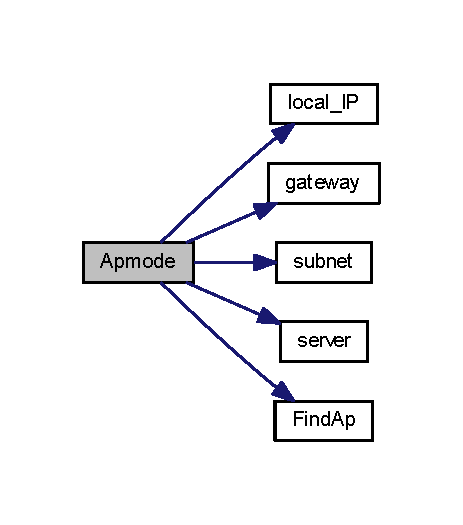
\includegraphics[width=222pt]{sl__uart__task_8c_ac923d0bf25ed513586077a218b54f4e5_cgraph}
\end{center}
\end{figure}
이 함수를 호출하는 함수들에 대한 그래프입니다.\+:\nopagebreak
\begin{figure}[H]
\begin{center}
\leavevmode
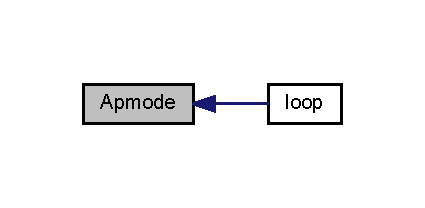
\includegraphics[width=204pt]{sl__uart__task_8c_ac923d0bf25ed513586077a218b54f4e5_icgraph}
\end{center}
\end{figure}
\mbox{\Hypertarget{sl__uart__task_8c_af273a6e233df1fa0ded638e07843b468}\label{sl__uart__task_8c_af273a6e233df1fa0ded638e07843b468}} 
\index{sl\+\_\+uart\+\_\+task.\+c@{sl\+\_\+uart\+\_\+task.\+c}!aws\+W\+Sclient@{aws\+W\+Sclient}}
\index{aws\+W\+Sclient@{aws\+W\+Sclient}!sl\+\_\+uart\+\_\+task.\+c@{sl\+\_\+uart\+\_\+task.\+c}}
\subsubsection{\texorpdfstring{aws\+W\+Sclient()}{awsWSclient()}}
{\footnotesize\ttfamily A\+W\+S\+Web\+Socket\+Client aws\+W\+Sclient (\begin{DoxyParamCaption}\item[{1024}]{ }\end{DoxyParamCaption})}

이 함수를 호출하는 함수들에 대한 그래프입니다.\+:\nopagebreak
\begin{figure}[H]
\begin{center}
\leavevmode
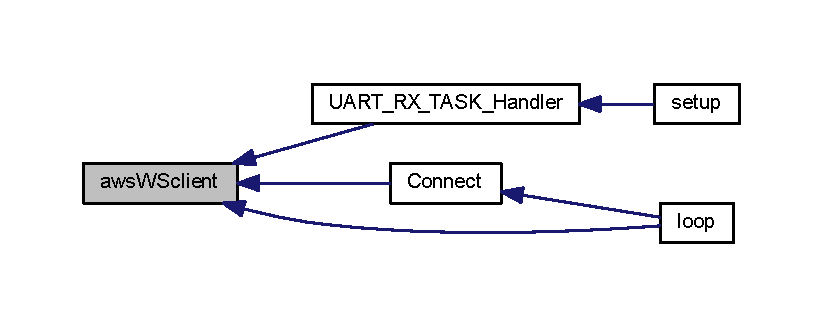
\includegraphics[width=350pt]{sl__uart__task_8c_af273a6e233df1fa0ded638e07843b468_icgraph}
\end{center}
\end{figure}
\mbox{\Hypertarget{sl__uart__task_8c_ac3a129f66dc859e2b7279565f4e1de78}\label{sl__uart__task_8c_ac3a129f66dc859e2b7279565f4e1de78}} 
\index{sl\+\_\+uart\+\_\+task.\+c@{sl\+\_\+uart\+\_\+task.\+c}!callback@{callback}}
\index{callback@{callback}!sl\+\_\+uart\+\_\+task.\+c@{sl\+\_\+uart\+\_\+task.\+c}}
\subsubsection{\texorpdfstring{callback()}{callback()}}
{\footnotesize\ttfamily void callback (\begin{DoxyParamCaption}\item[{char $\ast$}]{topic,  }\item[{byte $\ast$}]{payload,  }\item[{unsigned int}]{length }\end{DoxyParamCaption})}



callback 함수 

받은 메시지를 길이만큼 버퍼에 담아 가공한다 \begin{DoxySeeAlso}{참고}
이 함수의 코드분석 내용
\begin{DoxyEnumerate}
\item payload로 받은 메시지 길이 만큼 msg에 복사한다~\newline

\item msg에서 \char`\"{}desired\char`\"{}문자열이 있는지 찾는다~\newline

\item 위의 문자열이 존재한다면, global 변수(int) \mbox{\hyperlink{sl__uart__task_8c_a9eaf86bfd30962df9aff407bd4840336}{g\+\_\+msg\+Send}} 값을 2로 한다~\newline

\item 다시 msg에서 \char`\"{}cmp\+A\+P\+P\char`\"{}라는 문자열이 있는지 찾고 그 포인터를 str로 연결한다~\newline

\item str에서 포인터를 특정 문자(\mbox{[},\mbox{]})를 만나도록 이동후 잘라서 그 값을 A\+S\+C\+I\+I값을 token에 넣는다~\newline

\item 그 token값이 1인 경우 \+: global 변수(bool) g\+\_\+b\+Appctl를 true로 대입한다~\newline

\item 다시 msg에서 \char`\"{}cmd\+E\+R\+V\char`\"{}라는 문자열이 있는지 찾고 그 포인터를 str로 연결한다~\newline

\item str에서 포인터를 특정 문자(\mbox{[},\mbox{]})를 만나도록 이동후 잘라서 그 값(\+A\+S\+C\+I\+I)을 token에 넣는다~\newline

\item 4번 반복하여 그 값(\+A\+S\+C\+I\+I)을 erv\mbox{[}4\mbox{]}에 넣는다~\newline

\item 다시 msg에서 \char`\"{}cmd\+F\+C\+U\char`\"{}라는 문자열이 있는지 찾고 그 포인터를 str로 연결한다~\newline

\item str에서 포인터를 특정 문자(\mbox{[},\mbox{]})를 만나도록 이동후 잘라서 그 값(\+A\+S\+C\+I\+I)을 token에 넣는다~\newline

\item 6번 반복하여 그 값(\+A\+S\+C\+I\+I)을 fcu\mbox{[}6\mbox{]}에 넣는다~\newline

\item fcu\mbox{[}5\mbox{]}의 1인 경우(\+F\+C\+U) \+: fcu checksum을 확인~\newline

\item checksum이 문제 없는 경우 \+: global 변수(char) \mbox{\hyperlink{sl__uart__task_8c_a073128b0e46bc8edcc1b5ea52715bddd}{g\+\_\+cmd}}\mbox{[}8\mbox{]}에 값을 세팅한다~\newline

\item fcu\mbox{[}5\mbox{]}의 0인 경우(\+E\+R\+V) \+: lobal 변수(char) \mbox{\hyperlink{sl__uart__task_8c_a073128b0e46bc8edcc1b5ea52715bddd}{g\+\_\+cmd}}\mbox{[}8\mbox{]}에 값을 세팅한다~\newline

\item lobal 변수(char) \mbox{\hyperlink{sl__uart__task_8c_a073128b0e46bc8edcc1b5ea52715bddd}{g\+\_\+cmd}}\mbox{[}8\mbox{]}에 값을 세팅한다~\newline

\end{DoxyEnumerate}
\end{DoxySeeAlso}

\begin{DoxyParams}{매개변수}
{\em topic} & subcriber가 정한 topic 위치 \\
\hline
{\em payload} & 받은 메시지 \\
\hline
{\em length} & 메시지 길이 \\
\hline
\end{DoxyParams}
\begin{DoxyReturn}{반환값}
-\/ 
\end{DoxyReturn}


sl\+\_\+uart\+\_\+task.\+c 파일의 415 번째 라인에서 정의되었습니다.


\begin{DoxyCode}
415                                                                \{
416   \textcolor{keywordtype}{char} msg[length];
417   memcpy(msg, payload, length);
418 
419   \textcolor{keywordtype}{char}* str;
420   \textcolor{keywordtype}{char}* token;
421 
422   byte fcu[6];byte erv[4];
423 
424   \textcolor{keywordflow}{if}(strstr(msg,\textcolor{stringliteral}{"desired"})!=NULL)\{
425     \mbox{\hyperlink{sl__uart__task_8c_a9eaf86bfd30962df9aff407bd4840336}{g\_msgSend}} = 2;
426     str = strstr(msg,\textcolor{stringliteral}{"cmdAPP"});
427     token = strtok(str+8,\textcolor{stringliteral}{"[,]"});
428 
429     \textcolor{keywordflow}{if}(token - 48)\{
430       \mbox{\hyperlink{sl__uart__task_8c_a0dc0281c6f27e62a5cb21cde5288a9a5}{DebugSerial}}.println(\textcolor{stringliteral}{"App is controlled"});
431       \mbox{\hyperlink{sl__uart__task_8c_a06be4e59ee6e13a5f54dba4c3f014ec5}{g\_bAppctl}} = \textcolor{keyword}{true};
432     \}
433     
434     \mbox{\hyperlink{sl__uart__task_8c_a0dc0281c6f27e62a5cb21cde5288a9a5}{DebugSerial}}.print(\textcolor{stringliteral}{"cmdAPP : "} + (String)token + \textcolor{stringliteral}{" cmdERV : "});
435     
436     
437     str = strstr(msg,\textcolor{stringliteral}{"cmdERV"});
438     token = strtok(str+8,\textcolor{stringliteral}{"[,]"});
439     
440     \textcolor{keywordflow}{for}(\textcolor{keywordtype}{int} i= 0; i < 4; i++)\{
441       String tobyte(token);
442       erv[i] = tobyte.toInt();
443       \mbox{\hyperlink{sl__uart__task_8c_a0dc0281c6f27e62a5cb21cde5288a9a5}{DebugSerial}}.print((String)erv[i] +\textcolor{stringliteral}{" "});
444       token = strtok(NULL,\textcolor{stringliteral}{","});
445     \}
446     \mbox{\hyperlink{sl__uart__task_8c_a0dc0281c6f27e62a5cb21cde5288a9a5}{DebugSerial}}.print(\textcolor{stringliteral}{" cmdFCU : "});
447     str = strstr(msg,\textcolor{stringliteral}{"cmdFCU"});
448     token = strtok(str+8,\textcolor{stringliteral}{"[,]"});
449     
450     \textcolor{keywordflow}{for}(\textcolor{keywordtype}{int} i = 0; i < 6 ; i++)\{
451       String tobyte(token);
452       fcu[i] = tobyte.toInt();
453       \mbox{\hyperlink{sl__uart__task_8c_a0dc0281c6f27e62a5cb21cde5288a9a5}{DebugSerial}}.print((String)fcu[i]+ \textcolor{stringliteral}{" "});
454       token = strtok(NULL,\textcolor{stringliteral}{","});
455     \}
456     
457     \textcolor{keywordflow}{if}(!fcu[5])\{
458       \textcolor{keywordflow}{if}(!(fcu[0] ^ fcu[1] ^ fcu[2] ^ fcu[3]^fcu[4]))\{
459         \mbox{\hyperlink{sl__uart__task_8c_a0dc0281c6f27e62a5cb21cde5288a9a5}{DebugSerial}}.println(\textcolor{stringliteral}{"FCU received"});
460         \mbox{\hyperlink{sl__uart__task_8c_a073128b0e46bc8edcc1b5ea52715bddd}{g\_cmd}}[0] = 0xc5;
461         \mbox{\hyperlink{sl__uart__task_8c_a073128b0e46bc8edcc1b5ea52715bddd}{g\_cmd}}[2] = fcu[0] | fcu[1];
462         \mbox{\hyperlink{sl__uart__task_8c_a073128b0e46bc8edcc1b5ea52715bddd}{g\_cmd}}[3] = fcu[2];
463         \mbox{\hyperlink{sl__uart__task_8c_a073128b0e46bc8edcc1b5ea52715bddd}{g\_cmd}}[4] = fcu[3];
464       \}
465     \}
466     \textcolor{keywordflow}{else}\{
467       \mbox{\hyperlink{sl__uart__task_8c_a0dc0281c6f27e62a5cb21cde5288a9a5}{DebugSerial}}.println(\textcolor{stringliteral}{"ERV received"});
468       \mbox{\hyperlink{sl__uart__task_8c_a073128b0e46bc8edcc1b5ea52715bddd}{g\_cmd}}[0] = 0xc7;
469       \mbox{\hyperlink{sl__uart__task_8c_a073128b0e46bc8edcc1b5ea52715bddd}{g\_cmd}}[2] = erv[0];
470       \mbox{\hyperlink{sl__uart__task_8c_a073128b0e46bc8edcc1b5ea52715bddd}{g\_cmd}}[3] = erv[1];
471       \mbox{\hyperlink{sl__uart__task_8c_a073128b0e46bc8edcc1b5ea52715bddd}{g\_cmd}}[4] = erv[2];
472     \}
473 
474     \mbox{\hyperlink{sl__uart__task_8c_a073128b0e46bc8edcc1b5ea52715bddd}{g\_cmd}}[1] = 0x00;
475     \mbox{\hyperlink{sl__uart__task_8c_a073128b0e46bc8edcc1b5ea52715bddd}{g\_cmd}}[5] = 0x11;
476     \mbox{\hyperlink{sl__uart__task_8c_a073128b0e46bc8edcc1b5ea52715bddd}{g\_cmd}}[6] = 0x00;
477     \mbox{\hyperlink{sl__uart__task_8c_a073128b0e46bc8edcc1b5ea52715bddd}{g\_cmd}}[7] = \mbox{\hyperlink{sl__uart__task_8c_a073128b0e46bc8edcc1b5ea52715bddd}{g\_cmd}}[0] ^ \mbox{\hyperlink{sl__uart__task_8c_a073128b0e46bc8edcc1b5ea52715bddd}{g\_cmd}}[1] ^ \mbox{\hyperlink{sl__uart__task_8c_a073128b0e46bc8edcc1b5ea52715bddd}{g\_cmd}}[2] ^ \mbox{\hyperlink{sl__uart__task_8c_a073128b0e46bc8edcc1b5ea52715bddd}{g\_cmd}}[3] ^ 
      \mbox{\hyperlink{sl__uart__task_8c_a073128b0e46bc8edcc1b5ea52715bddd}{g\_cmd}}[4] ^ \mbox{\hyperlink{sl__uart__task_8c_a073128b0e46bc8edcc1b5ea52715bddd}{g\_cmd}}[5] ^ \mbox{\hyperlink{sl__uart__task_8c_a073128b0e46bc8edcc1b5ea52715bddd}{g\_cmd}}[6] ;
478   \}
479 \}
\end{DoxyCode}
이 함수를 호출하는 함수들에 대한 그래프입니다.\+:\nopagebreak
\begin{figure}[H]
\begin{center}
\leavevmode
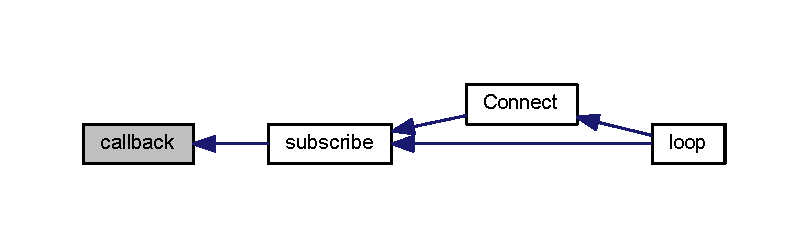
\includegraphics[width=350pt]{sl__uart__task_8c_ac3a129f66dc859e2b7279565f4e1de78_icgraph}
\end{center}
\end{figure}
\mbox{\Hypertarget{sl__uart__task_8c_ac4dd7f628ac36ff312d47a898d0573d6}\label{sl__uart__task_8c_ac4dd7f628ac36ff312d47a898d0573d6}} 
\index{sl\+\_\+uart\+\_\+task.\+c@{sl\+\_\+uart\+\_\+task.\+c}!Check\+Eeprom@{Check\+Eeprom}}
\index{Check\+Eeprom@{Check\+Eeprom}!sl\+\_\+uart\+\_\+task.\+c@{sl\+\_\+uart\+\_\+task.\+c}}
\subsubsection{\texorpdfstring{Check\+Eeprom()}{CheckEeprom()}}
{\footnotesize\ttfamily void Check\+Eeprom (\begin{DoxyParamCaption}\item[{void}]{ }\end{DoxyParamCaption})}



E\+E\+P\+R\+OM 체크 함수 

global 구조체 g\+\_\+\+Wall\+Pad s\+Init\+Chk 값과 global 배열\mbox{[}char\mbox{]} g\+\_\+s\+Init\+Title 값을 비교한다 \begin{DoxySeeAlso}{참고}
이 함수의 코드분석 내용
\begin{DoxyEnumerate}
\item E\+E\+P\+R\+OM 읽기 함수를 호출한다~\newline

\item global 구조체 \mbox{\hyperlink{sl__uart__task_8c_a45bb259cfa999c850530718ccac5609b}{g\+\_\+\+Wall\+Pad}} s\+Init\+Chk 값과 global 배열\mbox{[}char\mbox{]} \mbox{\hyperlink{sl__uart__task_8c_a888896fba8b48ebf2107d770e642e37f}{g\+\_\+s\+Init\+Title}} 값을 비교한다~\newline

\item 두 값이 일치하지 않는다면, E\+E\+P\+R\+OM 초기화 함수를 호출 후 E\+E\+P\+R\+OM 쓰기 함수를 호출한다 
\end{DoxyEnumerate}
\end{DoxySeeAlso}

\begin{DoxyParams}{매개변수}
{\em -\/} & \\
\hline
\end{DoxyParams}
\begin{DoxyReturn}{반환값}
-\/ 
\end{DoxyReturn}


sl\+\_\+uart\+\_\+task.\+c 파일의 654 번째 라인에서 정의되었습니다.


\begin{DoxyCode}
655 \{
656   \mbox{\hyperlink{sl__uart__task_8c_a0dc0281c6f27e62a5cb21cde5288a9a5}{DebugSerial}}.println(\textcolor{stringliteral}{"loading"});
657 
658   \mbox{\hyperlink{sl__uart__task_8c_a707a658761cc8b67188a0eb67ba9103e}{LoadEeprom}}();
659 
660   \mbox{\hyperlink{sl__uart__task_8c_a0dc0281c6f27e62a5cb21cde5288a9a5}{DebugSerial}}.println(\mbox{\hyperlink{sl__uart__task_8c_a45bb259cfa999c850530718ccac5609b}{g\_WallPad}}.\mbox{\hyperlink{struct_st_wall_pad_afa1dc1e2339538ae37ff115251ce1187}{sInitChk}});
661   \textcolor{keywordflow}{if}( strcmp( \mbox{\hyperlink{sl__uart__task_8c_a888896fba8b48ebf2107d770e642e37f}{g\_sInitTitle}}, \mbox{\hyperlink{sl__uart__task_8c_a45bb259cfa999c850530718ccac5609b}{g\_WallPad}}.\mbox{\hyperlink{struct_st_wall_pad_afa1dc1e2339538ae37ff115251ce1187}{sInitChk}} ) )
662   \{
663     \mbox{\hyperlink{sl__uart__task_8c_a0dc0281c6f27e62a5cb21cde5288a9a5}{DebugSerial}}.println(\textcolor{stringliteral}{"start init"});
664     \mbox{\hyperlink{sl__uart__task_8c_aed00320e0a0898df9eed984a3ced0ad8}{InitEeprom}}();
665     \mbox{\hyperlink{sl__uart__task_8c_a77d6a883c5cf0c92dcc225685249e38e}{StoreEeprom}}();
666   \}
667 \}
\end{DoxyCode}
이 함수 내부에서 호출하는 함수들에 대한 그래프입니다.\+:\nopagebreak
\begin{figure}[H]
\begin{center}
\leavevmode
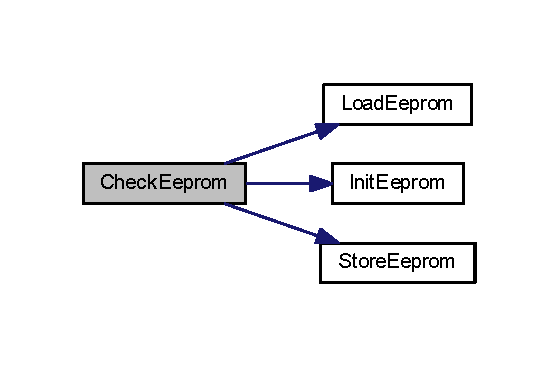
\includegraphics[width=268pt]{sl__uart__task_8c_ac4dd7f628ac36ff312d47a898d0573d6_cgraph}
\end{center}
\end{figure}
이 함수를 호출하는 함수들에 대한 그래프입니다.\+:\nopagebreak
\begin{figure}[H]
\begin{center}
\leavevmode
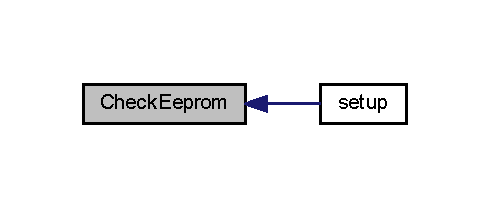
\includegraphics[width=235pt]{sl__uart__task_8c_ac4dd7f628ac36ff312d47a898d0573d6_icgraph}
\end{center}
\end{figure}
\mbox{\Hypertarget{sl__uart__task_8c_a38f7f9361dece3c36092a307f845f0a6}\label{sl__uart__task_8c_a38f7f9361dece3c36092a307f845f0a6}} 
\index{sl\+\_\+uart\+\_\+task.\+c@{sl\+\_\+uart\+\_\+task.\+c}!checksum@{checksum}}
\index{checksum@{checksum}!sl\+\_\+uart\+\_\+task.\+c@{sl\+\_\+uart\+\_\+task.\+c}}
\subsubsection{\texorpdfstring{checksum()}{checksum()}}
{\footnotesize\ttfamily int checksum (\begin{DoxyParamCaption}\item[{char $\ast$}]{data }\end{DoxyParamCaption})}



오류 확인 함수 

파라미터 data를 가지고 checksum 판단 
\begin{DoxyParams}{매개변수}
{\em char} & $\ast$ data \\
\hline
\end{DoxyParams}
\begin{DoxyReturn}{반환값}
int 0 \+: OK / 1 \+: Fail 
\end{DoxyReturn}


sl\+\_\+uart\+\_\+task.\+c 파일의 122 번째 라인에서 정의되었습니다.


\begin{DoxyCode}
122                         \{
123   \textcolor{keywordflow}{if}(data[0]^data[1]^data[2]^data[3]^data[4]^data[5]^data[6]^data[7])
124     \textcolor{keywordflow}{return} 0;
125   \textcolor{keywordflow}{else}
126     \textcolor{keywordflow}{return} 1;
127 \}
\end{DoxyCode}
이 함수를 호출하는 함수들에 대한 그래프입니다.\+:\nopagebreak
\begin{figure}[H]
\begin{center}
\leavevmode
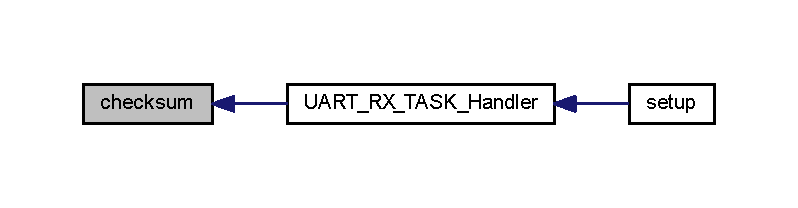
\includegraphics[width=350pt]{sl__uart__task_8c_a38f7f9361dece3c36092a307f845f0a6_icgraph}
\end{center}
\end{figure}
\mbox{\Hypertarget{sl__uart__task_8c_aed38f3e7ee0565ea6703f91a12983f54}\label{sl__uart__task_8c_aed38f3e7ee0565ea6703f91a12983f54}} 
\index{sl\+\_\+uart\+\_\+task.\+c@{sl\+\_\+uart\+\_\+task.\+c}!client@{client}}
\index{client@{client}!sl\+\_\+uart\+\_\+task.\+c@{sl\+\_\+uart\+\_\+task.\+c}}
\subsubsection{\texorpdfstring{client()}{client()}}
{\footnotesize\ttfamily Pub\+Sub\+Client client (\begin{DoxyParamCaption}\item[{\mbox{\hyperlink{sl__uart__task_8c_af273a6e233df1fa0ded638e07843b468}{aws\+W\+Sclient}}}]{ }\end{DoxyParamCaption})}

이 함수를 호출하는 함수들에 대한 그래프입니다.\+:\nopagebreak
\begin{figure}[H]
\begin{center}
\leavevmode
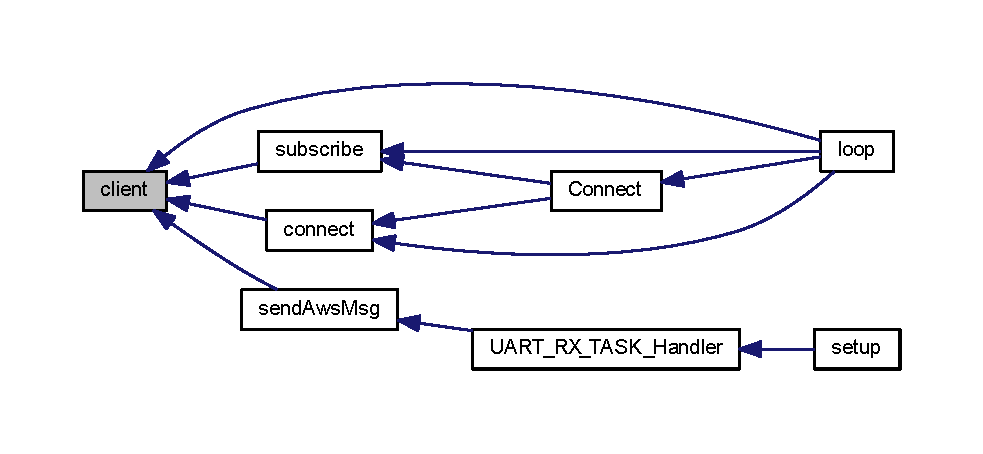
\includegraphics[width=350pt]{sl__uart__task_8c_aed38f3e7ee0565ea6703f91a12983f54_icgraph}
\end{center}
\end{figure}
\mbox{\Hypertarget{sl__uart__task_8c_aa0a57e883c6c9fc19e62a609d967be9c}\label{sl__uart__task_8c_aa0a57e883c6c9fc19e62a609d967be9c}} 
\index{sl\+\_\+uart\+\_\+task.\+c@{sl\+\_\+uart\+\_\+task.\+c}!connect@{connect}}
\index{connect@{connect}!sl\+\_\+uart\+\_\+task.\+c@{sl\+\_\+uart\+\_\+task.\+c}}
\subsubsection{\texorpdfstring{connect()}{connect()}}
{\footnotesize\ttfamily bool connect (\begin{DoxyParamCaption}{ }\end{DoxyParamCaption})}



websocket \& M\+Q\+TT 접속 함수 

클라이언트 I\+D를 가지고 서버(server)에 접속한다 \begin{DoxySeeAlso}{참고}
이 함수의 코드분석 내용
\begin{DoxyEnumerate}
\item 이미 접속되어있는지 판단하고 되어있으면 연결을 끊는다~\newline

\item 딜레이 함수 실행 \+: 힙 공간을 안전하게 확보~\newline

\item 클라이언트 ID 자동생성 함수를 가지고 ID 확보~\newline

\item 서버 연결하기 위한 서버 주소와 포트 설정~\newline

\item 클라이언트 I\+D로 접속되어있는지 판단 
\end{DoxyEnumerate}
\end{DoxySeeAlso}

\begin{DoxyParams}{매개변수}
{\em -\/} & \\
\hline
\end{DoxyParams}
\begin{DoxyReturn}{반환값}
bool OK / Fail 
\end{DoxyReturn}


sl\+\_\+uart\+\_\+task.\+c 파일의 289 번째 라인에서 정의되었습니다.


\begin{DoxyCode}
289                 \{
290   
291     \textcolor{keywordflow}{if} (\mbox{\hyperlink{sl__uart__task_8c_aed38f3e7ee0565ea6703f91a12983f54}{client}}.connected()) \{    
292         \mbox{\hyperlink{sl__uart__task_8c_aed38f3e7ee0565ea6703f91a12983f54}{client}}.disconnect ();
293     \}  
294     \textcolor{comment}{//delay is not necessary... it just help us to get a "trustful" heap space value}
295     delay (1000);
296     \mbox{\hyperlink{sl__uart__task_8c_a0dc0281c6f27e62a5cb21cde5288a9a5}{DebugSerial}}.print (millis ());
297     \mbox{\hyperlink{sl__uart__task_8c_a0dc0281c6f27e62a5cb21cde5288a9a5}{DebugSerial}}.print (\textcolor{stringliteral}{" - conn: "});
298     \mbox{\hyperlink{sl__uart__task_8c_a0dc0281c6f27e62a5cb21cde5288a9a5}{DebugSerial}}.print (++\mbox{\hyperlink{sl__uart__task_8c_ad268c14b4a9086cd1b67ca1d86f417d5}{connection}});
299     \mbox{\hyperlink{sl__uart__task_8c_a0dc0281c6f27e62a5cb21cde5288a9a5}{DebugSerial}}.print (\textcolor{stringliteral}{" - ("});
300     \mbox{\hyperlink{sl__uart__task_8c_a0dc0281c6f27e62a5cb21cde5288a9a5}{DebugSerial}}.print (ESP.getFreeHeap ());
301     \mbox{\hyperlink{sl__uart__task_8c_a0dc0281c6f27e62a5cb21cde5288a9a5}{DebugSerial}}.println (\textcolor{stringliteral}{")"});
302 
303 
304     \textcolor{comment}{//creating random client id}
305     \textcolor{keywordtype}{char}* clientID = \mbox{\hyperlink{sl__uart__task_8c_a0db6cddb7699ddbce4aa6f489d7d7879}{generateClientID}} ();
306     
307     \mbox{\hyperlink{sl__uart__task_8c_aed38f3e7ee0565ea6703f91a12983f54}{client}}.setServer(\mbox{\hyperlink{sl__uart__task_8c_a0977a0891557a2a5f83b635e5eb3443e}{aws\_endpoint}}, \mbox{\hyperlink{sl__uart__task_8c_a63c89c04d1feae07ca35558055155ffb}{port}});
308     \textcolor{keywordflow}{if} (\mbox{\hyperlink{sl__uart__task_8c_aed38f3e7ee0565ea6703f91a12983f54}{client}}.connect(clientID)) \{
309       \mbox{\hyperlink{sl__uart__task_8c_a0dc0281c6f27e62a5cb21cde5288a9a5}{DebugSerial}}.println(\textcolor{stringliteral}{"connected"});     
310       \textcolor{keywordflow}{return} \textcolor{keyword}{true};
311     \} \textcolor{keywordflow}{else} \{
312       \mbox{\hyperlink{sl__uart__task_8c_a0dc0281c6f27e62a5cb21cde5288a9a5}{DebugSerial}}.print(\textcolor{stringliteral}{"failed, rc="});
313       \mbox{\hyperlink{sl__uart__task_8c_a0dc0281c6f27e62a5cb21cde5288a9a5}{DebugSerial}}.print(\mbox{\hyperlink{sl__uart__task_8c_aed38f3e7ee0565ea6703f91a12983f54}{client}}.state());
314       \textcolor{keywordflow}{return} \textcolor{keyword}{false};
315     \}
316     
317 \}
\end{DoxyCode}
이 함수 내부에서 호출하는 함수들에 대한 그래프입니다.\+:\nopagebreak
\begin{figure}[H]
\begin{center}
\leavevmode
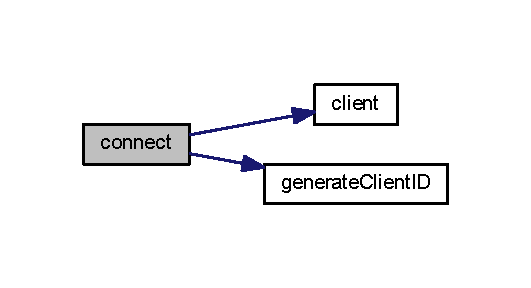
\includegraphics[width=255pt]{sl__uart__task_8c_aa0a57e883c6c9fc19e62a609d967be9c_cgraph}
\end{center}
\end{figure}
이 함수를 호출하는 함수들에 대한 그래프입니다.\+:\nopagebreak
\begin{figure}[H]
\begin{center}
\leavevmode
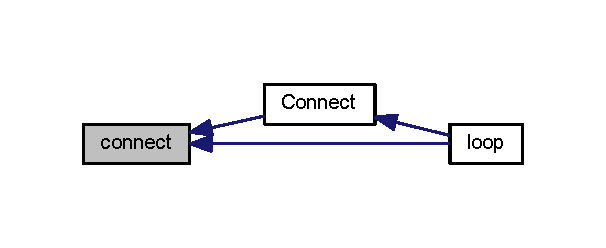
\includegraphics[width=291pt]{sl__uart__task_8c_aa0a57e883c6c9fc19e62a609d967be9c_icgraph}
\end{center}
\end{figure}
\mbox{\Hypertarget{sl__uart__task_8c_a5b6b4e47c7e5a413015c702d9825734f}\label{sl__uart__task_8c_a5b6b4e47c7e5a413015c702d9825734f}} 
\index{sl\+\_\+uart\+\_\+task.\+c@{sl\+\_\+uart\+\_\+task.\+c}!Connect@{Connect}}
\index{Connect@{Connect}!sl\+\_\+uart\+\_\+task.\+c@{sl\+\_\+uart\+\_\+task.\+c}}
\subsubsection{\texorpdfstring{Connect()}{Connect()}}
{\footnotesize\ttfamily void Connect (\begin{DoxyParamCaption}{ }\end{DoxyParamCaption})}



wifi \& aws 접속 함수 

신호가 가장 강력한 wifi를 잡아서 연결하고 A\+W\+S의 양식의 채운 후 aws와도 연결한다 \begin{DoxySeeAlso}{참고}
이 함수의 코드분석 내용
\begin{DoxyEnumerate}
\item wifi의 mode를 station으로 바꾼다~\newline

\item 프로그램이 돌리기 시작한 후 지난 밀리 초 숫자 값을 변수(long) conn\+\_\+prev\+\_\+time에 대입한다~\newline

\item A\+P에 접속하기 위해 global 배열\mbox{[}char\mbox{]} g\+\_\+s\+Init\+Ssid과 global 배열\mbox{[}char\mbox{]} g\+\_\+s\+Init\+Sspass를 사용한다~\newline

\item wifi 상태가 W\+L\+\_\+\+C\+O\+N\+N\+E\+C\+T\+E\+D과 같지 않을때까지 계속 반복하고, 프로그램이 돌리기 시작한 후 지난 밀리 초 숫자 값이 conn\+\_\+prev\+\_\+time보다 20000보다 클 경우~\newline
 wifi 연결진행을 중단하고 global 변수(bool) g\+\_\+b\+Connecting를 false로 변환한다~\newline

\item 위의 반복 조건으로 인해 global 변수(bool) g\+\_\+b\+Connecting를 true로 변환한다~\newline

\item wifi 상태가 W\+L\+\_\+\+C\+O\+N\+N\+E\+C\+T\+E\+D이라면 global 구조체 g\+\_\+\+Wall\+Pad의 s\+Ss\+Id, s\+Ss\+Pass값을 g\+\_\+s\+Init\+Ssid과 g\+\_\+s\+Init\+Sspass값으로 복사한다~\newline

\item E\+E\+P\+R\+OM 쓰기 함수를 호출한다~\newline

\item 클라이언트에게 \char`\"{}\+S\+P\+H\+I\+O\+T0010020200040000\char`\"{} 문자열을 보낸다~\newline

\item aws관한 정보를 채운다 (Region, domain, Key\+ID, Secretkey, ssl 사용유/무)~\newline

\item websocket \& M\+Q\+TT 접속 함수를 호출하고 클라이언트 I\+D로 접속되었다면 M\+Q\+TT \mbox{\hyperlink{sl__uart__task_8c_a0bccd94c4239c019c480e507cb6159ee}{subscribe}} 함수를 호출한다~\newline

\item g\+\_\+\+Wall\+Pad의 e\+Mode값을 e\+M\+O\+D\+E\+\_\+\+N\+O\+R\+M\+A\+L로 변환한다~\newline

\item 클라이언트와 서버 연결을 끊는다~\newline

\item wifi의 mode를 station으로 바꾼다~\newline

\item wifi 상태가 W\+L\+\_\+\+C\+O\+N\+N\+E\+C\+T\+E\+D아니라면, 클라이언트에게 \char`\"{}\+S\+P\+H\+I\+O\+T0010020200040001\char`\"{} 문자열을 보낸다~\newline

\item g\+\_\+\+Wall\+Pad의 e\+Mode값을 e\+M\+O\+D\+E\+\_\+\+A\+P로 변환한다~\newline

\item 클라이언트와 서버 연결을 끊는다~\newline

\item wifi의 mode를 W\+I\+F\+I\+\_\+\+O\+F\+F으로 바꾼다~\newline
 
\end{DoxyEnumerate}
\end{DoxySeeAlso}

\begin{DoxyParams}{매개변수}
{\em -\/} & \\
\hline
\end{DoxyParams}
\begin{DoxyReturn}{반환값}
-\/ 
\end{DoxyReturn}


sl\+\_\+uart\+\_\+task.\+c 파일의 932 번째 라인에서 정의되었습니다.


\begin{DoxyCode}
932               \{
933   WiFi.mode(WIFI\_STA);
934   \textcolor{keywordtype}{unsigned} \textcolor{keywordtype}{long} conn\_prev\_time = millis();
935   ESP8266WiFiMulti \mbox{\hyperlink{sl__uart__task_8c_a17dc5624a7578d8675ef9fed1b260754}{WiFiMulti}};
936   \mbox{\hyperlink{sl__uart__task_8c_a17dc5624a7578d8675ef9fed1b260754}{WiFiMulti}}.addAP(\mbox{\hyperlink{sl__uart__task_8c_aa5d0ec846e4a5c3218b26ac91b89c137}{g\_sInitSsid}}, \mbox{\hyperlink{sl__uart__task_8c_a1bdc597aadbd6a0b8f8ddfdc4aee425e}{g\_sInitSspass}});
937   \mbox{\hyperlink{sl__uart__task_8c_a0dc0281c6f27e62a5cb21cde5288a9a5}{DebugSerial}}.println (\textcolor{stringliteral}{"connecting to wifi"});
938 
939   \mbox{\hyperlink{sl__uart__task_8c_a0dc0281c6f27e62a5cb21cde5288a9a5}{DebugSerial}}.println(\mbox{\hyperlink{sl__uart__task_8c_aa5d0ec846e4a5c3218b26ac91b89c137}{g\_sInitSsid}});
940   \mbox{\hyperlink{sl__uart__task_8c_a0dc0281c6f27e62a5cb21cde5288a9a5}{DebugSerial}}.println(\mbox{\hyperlink{sl__uart__task_8c_a1bdc597aadbd6a0b8f8ddfdc4aee425e}{g\_sInitSspass}});
941 
942   
943   \textcolor{keywordflow}{while}(\mbox{\hyperlink{sl__uart__task_8c_a17dc5624a7578d8675ef9fed1b260754}{WiFiMulti}}.run() != WL\_CONNECTED ) \{
944     delay(100);
945     \mbox{\hyperlink{sl__uart__task_8c_a0dc0281c6f27e62a5cb21cde5288a9a5}{DebugSerial}}.print (\textcolor{stringliteral}{"."});
946     \textcolor{keywordflow}{if}(millis() - conn\_prev\_time > 20000)\{
947       \mbox{\hyperlink{sl__uart__task_8c_a0dc0281c6f27e62a5cb21cde5288a9a5}{DebugSerial}}.println (\textcolor{stringliteral}{"\(\backslash\)nconnecting time out"});
948       WiFi.disconnect();
949       \textcolor{keywordflow}{break};
950     \}
951     \mbox{\hyperlink{sl__uart__task_8c_aa557e6b05fc785e99ccfc9b09bc79bc5}{g\_bConnecting}} = \textcolor{keyword}{true};
952   \}
953   \mbox{\hyperlink{sl__uart__task_8c_aa557e6b05fc785e99ccfc9b09bc79bc5}{g\_bConnecting}} = \textcolor{keyword}{false};
954 
955   \textcolor{keywordflow}{if}(\mbox{\hyperlink{sl__uart__task_8c_a17dc5624a7578d8675ef9fed1b260754}{WiFiMulti}}.run() == WL\_CONNECTED)\{
956     strcpy( \mbox{\hyperlink{sl__uart__task_8c_a45bb259cfa999c850530718ccac5609b}{g\_WallPad}}.\mbox{\hyperlink{struct_st_wall_pad_afb1618185a1aecb8c77eff2f1453c24f}{sSsId}}     , \mbox{\hyperlink{sl__uart__task_8c_aa5d0ec846e4a5c3218b26ac91b89c137}{g\_sInitSsid}}   );
957     strcpy( \mbox{\hyperlink{sl__uart__task_8c_a45bb259cfa999c850530718ccac5609b}{g\_WallPad}}.\mbox{\hyperlink{struct_st_wall_pad_a8c77e9b61d65201646350d01f8a8d7c0}{sSsPass}}   , \mbox{\hyperlink{sl__uart__task_8c_a1bdc597aadbd6a0b8f8ddfdc4aee425e}{g\_sInitSspass}}   );
958     \mbox{\hyperlink{sl__uart__task_8c_a77d6a883c5cf0c92dcc225685249e38e}{StoreEeprom}}();
959 
960     \mbox{\hyperlink{sl__uart__task_8c_abbb6f0d4140565a3f0e833a4dc0ca10e}{tcpclient}}.print(\textcolor{stringliteral}{"SPHIOT0010020200040000"});
961     \mbox{\hyperlink{sl__uart__task_8c_a0dc0281c6f27e62a5cb21cde5288a9a5}{DebugSerial}}.print(\textcolor{stringliteral}{"SPHIOT0010020200040000"});
962     \mbox{\hyperlink{sl__uart__task_8c_a0dc0281c6f27e62a5cb21cde5288a9a5}{DebugSerial}}.println (\textcolor{stringliteral}{"\(\backslash\)nconnected"});
963 
964     \textcolor{comment}{//fill AWS parameters    }
965     \mbox{\hyperlink{sl__uart__task_8c_af273a6e233df1fa0ded638e07843b468}{awsWSclient}}.setAWSRegion(\mbox{\hyperlink{sl__uart__task_8c_a3c3e0be700ab12b748d8c833ee2255a1}{aws\_region}});
966     \mbox{\hyperlink{sl__uart__task_8c_af273a6e233df1fa0ded638e07843b468}{awsWSclient}}.setAWSDomain(\mbox{\hyperlink{sl__uart__task_8c_a0977a0891557a2a5f83b635e5eb3443e}{aws\_endpoint}});
967     \mbox{\hyperlink{sl__uart__task_8c_af273a6e233df1fa0ded638e07843b468}{awsWSclient}}.setAWSKeyID(\mbox{\hyperlink{sl__uart__task_8c_a45bf1e976b70d29f3c109c37a3b01b88}{aws\_key}});
968     \mbox{\hyperlink{sl__uart__task_8c_af273a6e233df1fa0ded638e07843b468}{awsWSclient}}.setAWSSecretKey(\mbox{\hyperlink{sl__uart__task_8c_a1297e4248f6e6a429598f485126a19ce}{aws\_secret}});
969     \mbox{\hyperlink{sl__uart__task_8c_af273a6e233df1fa0ded638e07843b468}{awsWSclient}}.setUseSSL(\textcolor{keyword}{true});
970 
971     \textcolor{keywordflow}{if} (\mbox{\hyperlink{sl__uart__task_8c_aa0a57e883c6c9fc19e62a609d967be9c}{connect}} ())\{
972       \mbox{\hyperlink{sl__uart__task_8c_a0bccd94c4239c019c480e507cb6159ee}{subscribe}} ();
973      \}
974 
975      \mbox{\hyperlink{sl__uart__task_8c_a45bb259cfa999c850530718ccac5609b}{g\_WallPad}}.\mbox{\hyperlink{struct_st_wall_pad_a51f947b3c4ad6a33d096bfaf1caedb6e}{eMode}} = \mbox{\hyperlink{_wall_pad_common_8h_a01baed20aab6218b9846cc7c935f8de9a25a620c7255a0d3a02bf847826791ce2}{eMODE\_NORMAL}};
976     \mbox{\hyperlink{sl__uart__task_8c_abbb6f0d4140565a3f0e833a4dc0ca10e}{tcpclient}}.stop();
977     WiFi.mode(WIFI\_STA);
978     return ;
979   \}
980 
981   \textcolor{keywordflow}{else}\{
982     \mbox{\hyperlink{sl__uart__task_8c_abbb6f0d4140565a3f0e833a4dc0ca10e}{tcpclient}}.print(\textcolor{stringliteral}{"SPHIOT0010020200040001"});
983     \mbox{\hyperlink{sl__uart__task_8c_a0dc0281c6f27e62a5cb21cde5288a9a5}{DebugSerial}}.print(\textcolor{stringliteral}{"SPHIOT0010020200040001"});
984     \mbox{\hyperlink{sl__uart__task_8c_a0dc0281c6f27e62a5cb21cde5288a9a5}{DebugSerial}}.println (\textcolor{stringliteral}{"\(\backslash\)nconnecting failed return to Ap mode"});
985     \mbox{\hyperlink{sl__uart__task_8c_a45bb259cfa999c850530718ccac5609b}{g\_WallPad}}.\mbox{\hyperlink{struct_st_wall_pad_a51f947b3c4ad6a33d096bfaf1caedb6e}{eMode}} = \mbox{\hyperlink{_wall_pad_common_8h_a01baed20aab6218b9846cc7c935f8de9a1f5cc10773bdfbec3b85c915572c4d8d}{eMODE\_AP}};
986   \}
987 
988   \mbox{\hyperlink{sl__uart__task_8c_abbb6f0d4140565a3f0e833a4dc0ca10e}{tcpclient}}.stop();
989   WiFi.mode(WIFI\_OFF);
990 
991 \}
\end{DoxyCode}
이 함수 내부에서 호출하는 함수들에 대한 그래프입니다.\+:\nopagebreak
\begin{figure}[H]
\begin{center}
\leavevmode
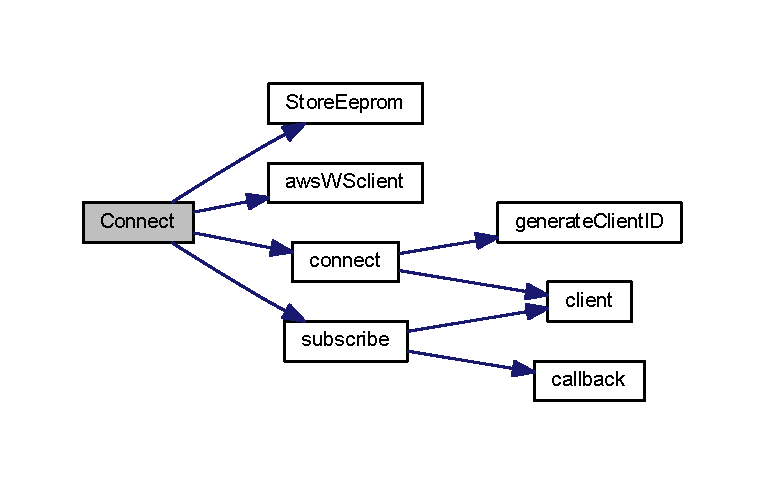
\includegraphics[width=350pt]{sl__uart__task_8c_a5b6b4e47c7e5a413015c702d9825734f_cgraph}
\end{center}
\end{figure}
이 함수를 호출하는 함수들에 대한 그래프입니다.\+:\nopagebreak
\begin{figure}[H]
\begin{center}
\leavevmode
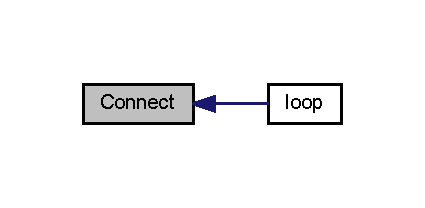
\includegraphics[width=204pt]{sl__uart__task_8c_a5b6b4e47c7e5a413015c702d9825734f_icgraph}
\end{center}
\end{figure}
\mbox{\Hypertarget{sl__uart__task_8c_a4476697452689e3561ad2909c9047f4a}\label{sl__uart__task_8c_a4476697452689e3561ad2909c9047f4a}} 
\index{sl\+\_\+uart\+\_\+task.\+c@{sl\+\_\+uart\+\_\+task.\+c}!Find\+Ap@{Find\+Ap}}
\index{Find\+Ap@{Find\+Ap}!sl\+\_\+uart\+\_\+task.\+c@{sl\+\_\+uart\+\_\+task.\+c}}
\subsubsection{\texorpdfstring{Find\+Ap()}{FindAp()}}
{\footnotesize\ttfamily int Find\+Ap (\begin{DoxyParamCaption}\item[{bool}]{ap }\end{DoxyParamCaption})}



wifi 신호 탐색 함수 

wifi로 접속할 수 있는 네트워크 장비를 탐색하고 식별\+I\+D와 신호감도 값을 저장한 후 신호감도에 따라 내림차순으로 정리하여 탐색을 마친다 \begin{DoxySeeAlso}{참고}
이 함수의 코드분석 내용
\begin{DoxyEnumerate}
\item 파라미터 ap 값이 false인 경우, wifi모드를 station으로 바꾸고 연결을 끊는다~\newline

\item 네트워크 장비를 탐색하고 탐색된 그 수를 global 변수(int) g\+\_\+n\+Max\+Ap에 반환한다~\newline

\item g\+\_\+n\+Max\+Ap만큼 반복하여 global 구조체배열 g\+\_\+\+Ap\+List의 s\+Ssid, n\+Rssi, b\+Encry값을 채운다~\newline

\item 신호 감도에 따라 내림차순으로 정리한다~\newline

\item 식별\+I\+D를 버퍼에 저장하고 global 구조체 g\+\_\+\+Wall\+Pad의 s\+Ss\+Id값과 비교한다~\newline

\item (g\+\_\+n\+Max\+Ap만큼 반복동안) 한번이라도 두 값이 동일하다면,~\newline
 global 배열\mbox{[}char\mbox{]} \mbox{\hyperlink{sl__uart__task_8c_aa5d0ec846e4a5c3218b26ac91b89c137}{g\+\_\+s\+Init\+Ssid}}, g\+\_\+s\+Init\+Sspass에 global 구조체 g\+\_\+\+Wall\+Pad의 s\+Ss\+Id과 s\+Ss\+Pass값을 복사하고 탐색을 마친다~\newline

\item g\+\_\+n\+Max\+Ap만큼 반복횟수동안 두 값이 불일치하다면 탐색을 마친다 
\end{DoxyEnumerate}
\end{DoxySeeAlso}

\begin{DoxyParams}{매개변수}
{\em bool} & ap \\
\hline
\end{DoxyParams}
\begin{DoxyReturn}{반환값}
int g\+\_\+n\+Max\+Ap \+: wifi로 접속할 수 있는 네트워크 장비 수 
\end{DoxyReturn}


sl\+\_\+uart\+\_\+task.\+c 파일의 694 번째 라인에서 정의되었습니다.


\begin{DoxyCode}
694                      \{
695   
696   \mbox{\hyperlink{sl__uart__task_8c_a0dc0281c6f27e62a5cb21cde5288a9a5}{DebugSerial}}.println(\textcolor{stringliteral}{"Find AP Scan Start"}+(String)ap);
697 
698   \textcolor{keywordflow}{if}(!ap)\{
699     WiFi.mode( WIFI\_STA );
700     WiFi.disconnect();
701     delay( 10 );
702   \}
703 
704   \mbox{\hyperlink{sl__uart__task_8c_a360ac0bcfdbb88764f1535bce0361cea}{g\_nMaxAp}} = WiFi.scanNetworks();
705   
706   \textcolor{keywordtype}{int} i, j;
707   
708   \textcolor{keywordflow}{for}( i=0; i < \mbox{\hyperlink{sl__uart__task_8c_a360ac0bcfdbb88764f1535bce0361cea}{g\_nMaxAp}}; i++ )
709   \{
710     \mbox{\hyperlink{sl__uart__task_8c_ab172c51f9996185c00e7eedc1f28b24a}{g\_ApList}}[ i ].\mbox{\hyperlink{struct_st_ap_list_a174040ae2c2468aa44f5c18ad915e7a3}{sSsid}}   = WiFi.SSID( i );
711     \mbox{\hyperlink{sl__uart__task_8c_ab172c51f9996185c00e7eedc1f28b24a}{g\_ApList}}[ i ].\mbox{\hyperlink{struct_st_ap_list_a04d6ede44986822269e924bb50a48369}{nRssi}}   = WiFi.RSSI( i );
712     \mbox{\hyperlink{sl__uart__task_8c_ab172c51f9996185c00e7eedc1f28b24a}{g\_ApList}}[ i ].\mbox{\hyperlink{struct_st_ap_list_a3491c9e85ee7dced99ca9b0ff6ea0327}{bEncry}}  = (WiFi.encryptionType( i ) == ENC\_TYPE\_NONE) ? \textcolor{keyword}{false} : \textcolor{keyword}{true};
713 
714     \mbox{\hyperlink{sl__uart__task_8c_a41db1cc0774aca1f9cbe536a9c5a518e}{g\_pApList}}[ i ] = &\mbox{\hyperlink{sl__uart__task_8c_ab172c51f9996185c00e7eedc1f28b24a}{g\_ApList}}[ i ];
715     delay( 10 );
716   \}
717   \mbox{\hyperlink{sl__uart__task_8c_a0dc0281c6f27e62a5cb21cde5288a9a5}{DebugSerial}}.println(\textcolor{stringliteral}{"p1"});
718   \textcolor{comment}{//Rssi sorting HIGH->LOW}
719   \mbox{\hyperlink{struct_st_ap_list}{pApList}} pTmp;
720   \textcolor{keywordflow}{for}( i=0; i < \mbox{\hyperlink{sl__uart__task_8c_a360ac0bcfdbb88764f1535bce0361cea}{g\_nMaxAp}} - 1; i++ )
721     \textcolor{keywordflow}{for}( j = i+1; j < \mbox{\hyperlink{sl__uart__task_8c_a360ac0bcfdbb88764f1535bce0361cea}{g\_nMaxAp}}; j++ )
722       \textcolor{keywordflow}{if}( \mbox{\hyperlink{sl__uart__task_8c_a41db1cc0774aca1f9cbe536a9c5a518e}{g\_pApList}}[ i ]->nRssi < \mbox{\hyperlink{sl__uart__task_8c_a41db1cc0774aca1f9cbe536a9c5a518e}{g\_pApList}}[ j ]->nRssi )
723       \{
724         pTmp = \mbox{\hyperlink{sl__uart__task_8c_a41db1cc0774aca1f9cbe536a9c5a518e}{g\_pApList}}[ i ];
725         \mbox{\hyperlink{sl__uart__task_8c_a41db1cc0774aca1f9cbe536a9c5a518e}{g\_pApList}}[ i ] = \mbox{\hyperlink{sl__uart__task_8c_a41db1cc0774aca1f9cbe536a9c5a518e}{g\_pApList}}[ j ];
726         \mbox{\hyperlink{sl__uart__task_8c_a41db1cc0774aca1f9cbe536a9c5a518e}{g\_pApList}}[ j ] = pTmp;
727       \}
728 
729   \mbox{\hyperlink{sl__uart__task_8c_a0dc0281c6f27e62a5cb21cde5288a9a5}{DebugSerial}}.println(\textcolor{stringliteral}{"p2"});
730     \textcolor{keywordflow}{for}( i=0; i < \mbox{\hyperlink{sl__uart__task_8c_a360ac0bcfdbb88764f1535bce0361cea}{g\_nMaxAp}} ; i++ )\{
731       \textcolor{keywordtype}{char} buf[30];
732       \mbox{\hyperlink{sl__uart__task_8c_a41db1cc0774aca1f9cbe536a9c5a518e}{g\_pApList}}[i]->\mbox{\hyperlink{struct_st_ap_list_a174040ae2c2468aa44f5c18ad915e7a3}{sSsid}}.toCharArray(buf, \mbox{\hyperlink{sl__uart__task_8c_a41db1cc0774aca1f9cbe536a9c5a518e}{g\_pApList}}[i]->sSsid.length()+1);
733       
734       \textcolor{keywordflow}{if}(ap)
735         \mbox{\hyperlink{sl__uart__task_8c_a0dc0281c6f27e62a5cb21cde5288a9a5}{DebugSerial}}.println(buf);
736 
737       \textcolor{keywordflow}{if}(!strcmp(\mbox{\hyperlink{sl__uart__task_8c_a45bb259cfa999c850530718ccac5609b}{g\_WallPad}}.\mbox{\hyperlink{struct_st_wall_pad_afb1618185a1aecb8c77eff2f1453c24f}{sSsId}},buf))\{
738         strcpy(\mbox{\hyperlink{sl__uart__task_8c_aa5d0ec846e4a5c3218b26ac91b89c137}{g\_sInitSsid}},\mbox{\hyperlink{sl__uart__task_8c_a45bb259cfa999c850530718ccac5609b}{g\_WallPad}}.\mbox{\hyperlink{struct_st_wall_pad_afb1618185a1aecb8c77eff2f1453c24f}{sSsId}});
739         strcpy(\mbox{\hyperlink{sl__uart__task_8c_a1bdc597aadbd6a0b8f8ddfdc4aee425e}{g\_sInitSspass}},\mbox{\hyperlink{sl__uart__task_8c_a45bb259cfa999c850530718ccac5609b}{g\_WallPad}}.\mbox{\hyperlink{struct_st_wall_pad_a8c77e9b61d65201646350d01f8a8d7c0}{sSsPass}});
740         WiFi.scanDelete();
741         
742         \textcolor{keywordflow}{return} 1;
743       \}
744 
745     \}
746     \mbox{\hyperlink{sl__uart__task_8c_a0dc0281c6f27e62a5cb21cde5288a9a5}{DebugSerial}}.println(\textcolor{stringliteral}{"p3"});
747  
748   WiFi.scanDelete();
749   \textcolor{keywordflow}{return} \mbox{\hyperlink{sl__uart__task_8c_a360ac0bcfdbb88764f1535bce0361cea}{g\_nMaxAp}};
750 \}
\end{DoxyCode}
이 함수를 호출하는 함수들에 대한 그래프입니다.\+:\nopagebreak
\begin{figure}[H]
\begin{center}
\leavevmode
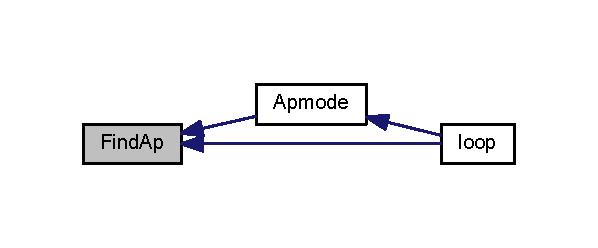
\includegraphics[width=287pt]{sl__uart__task_8c_a4476697452689e3561ad2909c9047f4a_icgraph}
\end{center}
\end{figure}
\mbox{\Hypertarget{sl__uart__task_8c_a140be8626580a0cb94729a6615877d40}\label{sl__uart__task_8c_a140be8626580a0cb94729a6615877d40}} 
\index{sl\+\_\+uart\+\_\+task.\+c@{sl\+\_\+uart\+\_\+task.\+c}!gateway@{gateway}}
\index{gateway@{gateway}!sl\+\_\+uart\+\_\+task.\+c@{sl\+\_\+uart\+\_\+task.\+c}}
\subsubsection{\texorpdfstring{gateway()}{gateway()}}
{\footnotesize\ttfamily I\+P\+Address gateway (\begin{DoxyParamCaption}\item[{192}]{,  }\item[{168}]{,  }\item[{1}]{,  }\item[{1}]{ }\end{DoxyParamCaption})}

이 함수를 호출하는 함수들에 대한 그래프입니다.\+:\nopagebreak
\begin{figure}[H]
\begin{center}
\leavevmode
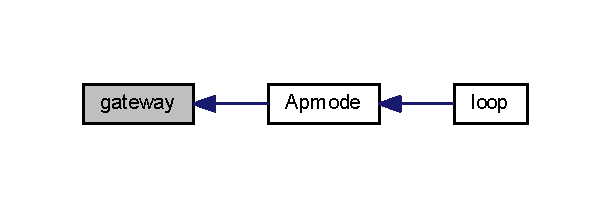
\includegraphics[width=293pt]{sl__uart__task_8c_a140be8626580a0cb94729a6615877d40_icgraph}
\end{center}
\end{figure}
\mbox{\Hypertarget{sl__uart__task_8c_a0db6cddb7699ddbce4aa6f489d7d7879}\label{sl__uart__task_8c_a0db6cddb7699ddbce4aa6f489d7d7879}} 
\index{sl\+\_\+uart\+\_\+task.\+c@{sl\+\_\+uart\+\_\+task.\+c}!generate\+Client\+ID@{generate\+Client\+ID}}
\index{generate\+Client\+ID@{generate\+Client\+ID}!sl\+\_\+uart\+\_\+task.\+c@{sl\+\_\+uart\+\_\+task.\+c}}
\subsubsection{\texorpdfstring{generate\+Client\+I\+D()}{generateClientID()}}
{\footnotesize\ttfamily char$\ast$ generate\+Client\+ID (\begin{DoxyParamCaption}{ }\end{DoxyParamCaption})}



클라이언트 ID 자동생성 함수 

랜덤함수를 가지고 1$\sim$256 사이 수의 숫자를 23개 만든다 
\begin{DoxyParams}{매개변수}
{\em -\/} & \\
\hline
\end{DoxyParams}
\begin{DoxyReturn}{반환값}
char $\ast$ \+: 클라이언트 ID 
\end{DoxyReturn}


sl\+\_\+uart\+\_\+task.\+c 파일의 268 번째 라인에서 정의되었습니다.


\begin{DoxyCode}
268                           \{
269   \textcolor{keywordtype}{char}* cID = \textcolor{keyword}{new} \textcolor{keywordtype}{char}[23]();
270   \textcolor{keywordflow}{for} (\textcolor{keywordtype}{int} i=0; i<22; i+=1)
271     cID[i]=(\textcolor{keywordtype}{char})random(1, 256);
272   \textcolor{keywordflow}{return} cID;
273 \}
\end{DoxyCode}
이 함수를 호출하는 함수들에 대한 그래프입니다.\+:\nopagebreak
\begin{figure}[H]
\begin{center}
\leavevmode
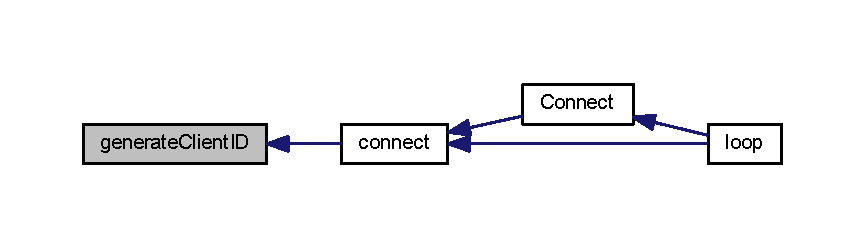
\includegraphics[width=350pt]{sl__uart__task_8c_a0db6cddb7699ddbce4aa6f489d7d7879_icgraph}
\end{center}
\end{figure}
\mbox{\Hypertarget{sl__uart__task_8c_aed00320e0a0898df9eed984a3ced0ad8}\label{sl__uart__task_8c_aed00320e0a0898df9eed984a3ced0ad8}} 
\index{sl\+\_\+uart\+\_\+task.\+c@{sl\+\_\+uart\+\_\+task.\+c}!Init\+Eeprom@{Init\+Eeprom}}
\index{Init\+Eeprom@{Init\+Eeprom}!sl\+\_\+uart\+\_\+task.\+c@{sl\+\_\+uart\+\_\+task.\+c}}
\subsubsection{\texorpdfstring{Init\+Eeprom()}{InitEeprom()}}
{\footnotesize\ttfamily void Init\+Eeprom (\begin{DoxyParamCaption}\item[{void}]{ }\end{DoxyParamCaption})}



E\+E\+P\+R\+OM 초기화 함수 

global 구조체 g\+\_\+\+Wall\+Pad 값을 정해진 값으로 세팅하고 그 구조체만큼 E\+E\+P\+R\+O\+M를 0으로 세팅한다 \begin{DoxySeeAlso}{참고}
이 함수의 코드분석 내용
\begin{DoxyEnumerate}
\item global 구조체 \mbox{\hyperlink{sl__uart__task_8c_a45bb259cfa999c850530718ccac5609b}{g\+\_\+\+Wall\+Pad}} e\+Mode를 값을 e\+Mode\+\_\+\+N\+O\+NE 대입한다~\newline

\item global 구조체 \mbox{\hyperlink{sl__uart__task_8c_a45bb259cfa999c850530718ccac5609b}{g\+\_\+\+Wall\+Pad}} s\+Init\+Chk 값을 global 배열\mbox{[}char\mbox{]} \mbox{\hyperlink{sl__uart__task_8c_a888896fba8b48ebf2107d770e642e37f}{g\+\_\+s\+Init\+Title}} 값으로 대입한다~\newline

\item global 구조체 \mbox{\hyperlink{sl__uart__task_8c_a45bb259cfa999c850530718ccac5609b}{g\+\_\+\+Wall\+Pad}} s\+Ss\+Id 값을 global 배열\mbox{[}char\mbox{]} \mbox{\hyperlink{sl__uart__task_8c_aa5d0ec846e4a5c3218b26ac91b89c137}{g\+\_\+s\+Init\+Ssid}} 값으로 대입한다~\newline

\item global 구조체 \mbox{\hyperlink{sl__uart__task_8c_a45bb259cfa999c850530718ccac5609b}{g\+\_\+\+Wall\+Pad}} s\+Ss\+Pass 값을 global 배열\mbox{[}char\mbox{]} \mbox{\hyperlink{sl__uart__task_8c_a1bdc597aadbd6a0b8f8ddfdc4aee425e}{g\+\_\+s\+Init\+Sspass}} 값으로 대입한다~\newline

\item global 구조체 \mbox{\hyperlink{sl__uart__task_8c_a45bb259cfa999c850530718ccac5609b}{g\+\_\+\+Wall\+Pad}} 크기만큼 E\+E\+P\+R\+O\+M를 0로 세팅한다 
\end{DoxyEnumerate}
\end{DoxySeeAlso}

\begin{DoxyParams}{매개변수}
{\em -\/} & \\
\hline
\end{DoxyParams}
\begin{DoxyReturn}{반환값}
-\/ 
\end{DoxyReturn}


sl\+\_\+uart\+\_\+task.\+c 파일의 595 번째 라인에서 정의되었습니다.


\begin{DoxyCode}
596 \{
597 
598   \mbox{\hyperlink{sl__uart__task_8c_a45bb259cfa999c850530718ccac5609b}{g\_WallPad}}.\mbox{\hyperlink{struct_st_wall_pad_a51f947b3c4ad6a33d096bfaf1caedb6e}{eMode}}   = \mbox{\hyperlink{_wall_pad_common_8h_a01baed20aab6218b9846cc7c935f8de9abb51c808160be71ef81bc5880610bedc}{eMODE\_NONE}};
599   strcpy( \mbox{\hyperlink{sl__uart__task_8c_a45bb259cfa999c850530718ccac5609b}{g\_WallPad}}.\mbox{\hyperlink{struct_st_wall_pad_afa1dc1e2339538ae37ff115251ce1187}{sInitChk}}    , \mbox{\hyperlink{sl__uart__task_8c_a888896fba8b48ebf2107d770e642e37f}{g\_sInitTitle}}    );
600   strcpy( \mbox{\hyperlink{sl__uart__task_8c_a45bb259cfa999c850530718ccac5609b}{g\_WallPad}}.\mbox{\hyperlink{struct_st_wall_pad_afb1618185a1aecb8c77eff2f1453c24f}{sSsId}}     , \mbox{\hyperlink{sl__uart__task_8c_aa5d0ec846e4a5c3218b26ac91b89c137}{g\_sInitSsid}}   );
601   strcpy( \mbox{\hyperlink{sl__uart__task_8c_a45bb259cfa999c850530718ccac5609b}{g\_WallPad}}.\mbox{\hyperlink{struct_st_wall_pad_a8c77e9b61d65201646350d01f8a8d7c0}{sSsPass}}   , \mbox{\hyperlink{sl__uart__task_8c_a1bdc597aadbd6a0b8f8ddfdc4aee425e}{g\_sInitSspass}}   );
602   \textcolor{keywordflow}{for}( \textcolor{keywordtype}{int} i= 0; i < \textcolor{keyword}{sizeof}( \mbox{\hyperlink{_wall_pad_common_8h_afc78910c4749fa1230e1149115f9d70a}{WallPad}} ); i++ )
603     EEPROM.write( i, 0 );
604   EEPROM.commit();
605 \}
\end{DoxyCode}
이 함수를 호출하는 함수들에 대한 그래프입니다.\+:\nopagebreak
\begin{figure}[H]
\begin{center}
\leavevmode
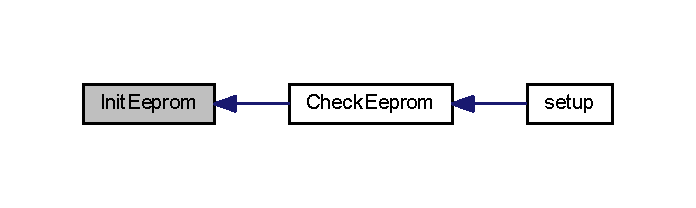
\includegraphics[width=334pt]{sl__uart__task_8c_aed00320e0a0898df9eed984a3ced0ad8_icgraph}
\end{center}
\end{figure}
\mbox{\Hypertarget{sl__uart__task_8c_a707a658761cc8b67188a0eb67ba9103e}\label{sl__uart__task_8c_a707a658761cc8b67188a0eb67ba9103e}} 
\index{sl\+\_\+uart\+\_\+task.\+c@{sl\+\_\+uart\+\_\+task.\+c}!Load\+Eeprom@{Load\+Eeprom}}
\index{Load\+Eeprom@{Load\+Eeprom}!sl\+\_\+uart\+\_\+task.\+c@{sl\+\_\+uart\+\_\+task.\+c}}
\subsubsection{\texorpdfstring{Load\+Eeprom()}{LoadEeprom()}}
{\footnotesize\ttfamily void Load\+Eeprom (\begin{DoxyParamCaption}\item[{void}]{ }\end{DoxyParamCaption})}



E\+E\+P\+R\+OM 읽기 함수 

E\+E\+P\+R\+O\+M의 값을 global 구조체 g\+\_\+\+Wall\+Pad로 불러들인다 \begin{DoxySeeAlso}{참고}
이 함수의 코드분석 내용
\begin{DoxyEnumerate}
\item global 구조체 g\+\_\+\+Wall\+Pad를 포인터로 연결한다~\newline

\item global 구조체 \mbox{\hyperlink{sl__uart__task_8c_a45bb259cfa999c850530718ccac5609b}{g\+\_\+\+Wall\+Pad}} 크기만큼 global 구조체 g\+\_\+\+Wall\+Pad를 E\+E\+P\+R\+OM 값으로 세팅한다 
\end{DoxyEnumerate}
\end{DoxySeeAlso}

\begin{DoxyParams}{매개변수}
{\em -\/} & \\
\hline
\end{DoxyParams}
\begin{DoxyReturn}{반환값}
-\/ 
\end{DoxyReturn}


sl\+\_\+uart\+\_\+task.\+c 파일의 634 번째 라인에서 정의되었습니다.


\begin{DoxyCode}
635 \{
636    \textcolor{keywordtype}{char}* pSetData = ( \textcolor{keywordtype}{char}*) &\mbox{\hyperlink{sl__uart__task_8c_a45bb259cfa999c850530718ccac5609b}{g\_WallPad}};
637   \textcolor{keywordtype}{int} i;
638   \textcolor{keywordflow}{for}( i=0; i < \textcolor{keyword}{sizeof}( \mbox{\hyperlink{_wall_pad_common_8h_afc78910c4749fa1230e1149115f9d70a}{WallPad}} ); i++ )\{
639     *pSetData++ = EEPROM.read( i );
640   \}
641   \mbox{\hyperlink{sl__uart__task_8c_a0dc0281c6f27e62a5cb21cde5288a9a5}{DebugSerial}}.println((String)pSetData);
642 \}
\end{DoxyCode}
이 함수를 호출하는 함수들에 대한 그래프입니다.\+:\nopagebreak
\begin{figure}[H]
\begin{center}
\leavevmode
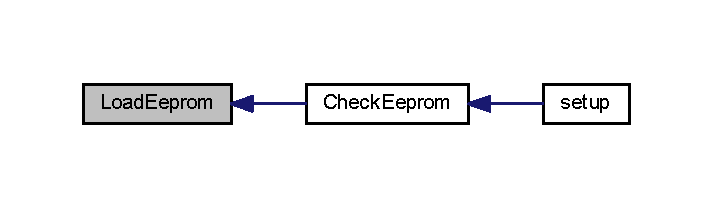
\includegraphics[width=342pt]{sl__uart__task_8c_a707a658761cc8b67188a0eb67ba9103e_icgraph}
\end{center}
\end{figure}
\mbox{\Hypertarget{sl__uart__task_8c_a70c83cd124803780a6e042045ec2d029}\label{sl__uart__task_8c_a70c83cd124803780a6e042045ec2d029}} 
\index{sl\+\_\+uart\+\_\+task.\+c@{sl\+\_\+uart\+\_\+task.\+c}!local\+\_\+\+IP@{local\+\_\+\+IP}}
\index{local\+\_\+\+IP@{local\+\_\+\+IP}!sl\+\_\+uart\+\_\+task.\+c@{sl\+\_\+uart\+\_\+task.\+c}}
\subsubsection{\texorpdfstring{local\+\_\+\+I\+P()}{local\_IP()}}
{\footnotesize\ttfamily I\+P\+Address local\+\_\+\+IP (\begin{DoxyParamCaption}\item[{192}]{,  }\item[{168}]{,  }\item[{1}]{,  }\item[{1}]{ }\end{DoxyParamCaption})}

이 함수를 호출하는 함수들에 대한 그래프입니다.\+:\nopagebreak
\begin{figure}[H]
\begin{center}
\leavevmode
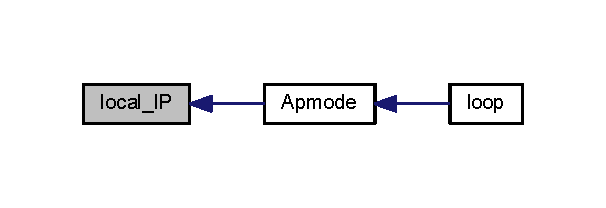
\includegraphics[width=291pt]{sl__uart__task_8c_a70c83cd124803780a6e042045ec2d029_icgraph}
\end{center}
\end{figure}
\mbox{\Hypertarget{sl__uart__task_8c_afe461d27b9c48d5921c00d521181f12f}\label{sl__uart__task_8c_afe461d27b9c48d5921c00d521181f12f}} 
\index{sl\+\_\+uart\+\_\+task.\+c@{sl\+\_\+uart\+\_\+task.\+c}!loop@{loop}}
\index{loop@{loop}!sl\+\_\+uart\+\_\+task.\+c@{sl\+\_\+uart\+\_\+task.\+c}}
\subsubsection{\texorpdfstring{loop()}{loop()}}
{\footnotesize\ttfamily void loop (\begin{DoxyParamCaption}{ }\end{DoxyParamCaption})}



e\+Mode 함수 

g\+\_\+\+Wall\+Pad의 e\+Mode값에 따라 분기점을 나누어서 원하는 조건에 실행하도록 한다 \begin{DoxySeeAlso}{참고}
이 함수의 코드분석 내용
\begin{DoxyEnumerate}
\item g\+\_\+\+Wall\+Pad의 e\+Mode값에 따라 스위치문으로 나눈다~\newline

\item \mbox{\hyperlink{_wall_pad_common_8h_a01baed20aab6218b9846cc7c935f8de9abb51c808160be71ef81bc5880610bedc}{e\+M\+O\+D\+E\+\_\+\+N\+O\+NE}} \+: g\+\_\+\+Wall\+Pad의 e\+Mode값을 e\+M\+O\+D\+E\+\_\+\+S\+E\+A\+R\+C\+H\+\_\+\+A\+P로 변환한다~\newline

\item \mbox{\hyperlink{_wall_pad_common_8h_a01baed20aab6218b9846cc7c935f8de9afbc0f8c6a5b25b698265ad7b74b9d9b7}{e\+M\+O\+D\+E\+\_\+\+S\+E\+A\+R\+C\+H\+\_\+\+AP}} \+: wifi 신호 탐색 함수를 호출하고 반환값이 1이면 e\+M\+O\+D\+E\+\_\+\+C\+O\+N\+N\+E\+C\+T값을 아니면 e\+M\+O\+D\+E\+\_\+\+A\+P값으로 변환한다~\newline

\item \mbox{\hyperlink{_wall_pad_common_8h_a01baed20aab6218b9846cc7c935f8de9a1f5cc10773bdfbec3b85c915572c4d8d}{e\+M\+O\+D\+E\+\_\+\+AP}} \+: wifi 서비스 함수를 호출한다~\newline

\item \mbox{\hyperlink{_wall_pad_common_8h_a01baed20aab6218b9846cc7c935f8de9ae9734b024c572803a9131d2df41dece2}{e\+M\+O\+D\+E\+\_\+\+C\+O\+N\+N\+E\+CT}} \+: websocket \& M\+Q\+TT 접속 함수를 호출한다~\newline

\item \mbox{\hyperlink{_wall_pad_common_8h_a01baed20aab6218b9846cc7c935f8de9a25a620c7255a0d3a02bf847826791ce2}{e\+M\+O\+D\+E\+\_\+\+N\+O\+R\+M\+AL}} \+: wifi가 연결되어있다면, 또 aws에도 연결이 되어있는지, 둘 다 되어있으면 e\+Mode 함수를 호출한다~\newline

\item \mbox{\hyperlink{_wall_pad_common_8h_a01baed20aab6218b9846cc7c935f8de9a25a620c7255a0d3a02bf847826791ce2}{e\+M\+O\+D\+E\+\_\+\+N\+O\+R\+M\+AL}} \+: aws가 연결이 안되어있다면, websocket \& M\+Q\+TT 접속 함수를 호출하고 반환값이 true이면 M\+Q\+TT \mbox{\hyperlink{sl__uart__task_8c_a0bccd94c4239c019c480e507cb6159ee}{subscribe}} 함수를 호출한다~\newline

\item \mbox{\hyperlink{_wall_pad_common_8h_a01baed20aab6218b9846cc7c935f8de9a25a620c7255a0d3a02bf847826791ce2}{e\+M\+O\+D\+E\+\_\+\+N\+O\+R\+M\+AL}} \+: wifi가 연결이 안되어 있다면, e\+M\+O\+D\+E\+\_\+\+C\+O\+N\+N\+E\+C\+T값으로 변환한다 
\end{DoxyEnumerate}
\end{DoxySeeAlso}

\begin{DoxyParams}{매개변수}
{\em -\/} & \\
\hline
\end{DoxyParams}
\begin{DoxyReturn}{반환값}
-\/ 
\end{DoxyReturn}


sl\+\_\+uart\+\_\+task.\+c 파일의 1068 번째 라인에서 정의되었습니다.


\begin{DoxyCode}
1068             \{
1069 
1070    \textcolor{keywordflow}{switch}(\mbox{\hyperlink{sl__uart__task_8c_a45bb259cfa999c850530718ccac5609b}{g\_WallPad}}.\mbox{\hyperlink{struct_st_wall_pad_a51f947b3c4ad6a33d096bfaf1caedb6e}{eMode}})\{
1071     
1072     \textcolor{keywordflow}{case} \mbox{\hyperlink{_wall_pad_common_8h_a01baed20aab6218b9846cc7c935f8de9abb51c808160be71ef81bc5880610bedc}{eMODE\_NONE}}:
1073       \mbox{\hyperlink{sl__uart__task_8c_a45bb259cfa999c850530718ccac5609b}{g\_WallPad}}.\mbox{\hyperlink{struct_st_wall_pad_a51f947b3c4ad6a33d096bfaf1caedb6e}{eMode}} = \mbox{\hyperlink{_wall_pad_common_8h_a01baed20aab6218b9846cc7c935f8de9afbc0f8c6a5b25b698265ad7b74b9d9b7}{eMODE\_SEARCH\_AP}};
1074       
1075     \textcolor{keywordflow}{break};
1076 
1077     \textcolor{keywordflow}{case} \mbox{\hyperlink{_wall_pad_common_8h_a01baed20aab6218b9846cc7c935f8de9afbc0f8c6a5b25b698265ad7b74b9d9b7}{eMODE\_SEARCH\_AP}}:
1078       \textcolor{keywordflow}{if}(\mbox{\hyperlink{sl__uart__task_8c_a4476697452689e3561ad2909c9047f4a}{FindAp}}(0) == 1)\{
1079         \mbox{\hyperlink{sl__uart__task_8c_a45bb259cfa999c850530718ccac5609b}{g\_WallPad}}.\mbox{\hyperlink{struct_st_wall_pad_a51f947b3c4ad6a33d096bfaf1caedb6e}{eMode}} = \mbox{\hyperlink{_wall_pad_common_8h_a01baed20aab6218b9846cc7c935f8de9ae9734b024c572803a9131d2df41dece2}{eMODE\_CONNECT}};  
1080       \}
1081       \textcolor{keywordflow}{else}\{
1082         \mbox{\hyperlink{sl__uart__task_8c_a45bb259cfa999c850530718ccac5609b}{g\_WallPad}}.\mbox{\hyperlink{struct_st_wall_pad_a51f947b3c4ad6a33d096bfaf1caedb6e}{eMode}} = \mbox{\hyperlink{_wall_pad_common_8h_a01baed20aab6218b9846cc7c935f8de9a1f5cc10773bdfbec3b85c915572c4d8d}{eMODE\_AP}};
1083       \}
1084     \textcolor{keywordflow}{break};
1085 
1086     \textcolor{keywordflow}{case} \mbox{\hyperlink{_wall_pad_common_8h_a01baed20aab6218b9846cc7c935f8de9a1f5cc10773bdfbec3b85c915572c4d8d}{eMODE\_AP}}:
1087       \mbox{\hyperlink{sl__uart__task_8c_ac923d0bf25ed513586077a218b54f4e5}{Apmode}}();
1088       
1089     \textcolor{keywordflow}{break};
1090 
1091     \textcolor{keywordflow}{case} \mbox{\hyperlink{_wall_pad_common_8h_a01baed20aab6218b9846cc7c935f8de9ae9734b024c572803a9131d2df41dece2}{eMODE\_CONNECT}}:
1092       \mbox{\hyperlink{sl__uart__task_8c_a5b6b4e47c7e5a413015c702d9825734f}{Connect}}();
1093     \textcolor{keywordflow}{break};
1094 
1095     \textcolor{keywordflow}{case} \mbox{\hyperlink{_wall_pad_common_8h_a01baed20aab6218b9846cc7c935f8de9a25a620c7255a0d3a02bf847826791ce2}{eMODE\_NORMAL}}:
1096       \textcolor{keywordflow}{if}(WiFi.isConnected())\{
1097         \textcolor{keywordflow}{if} (\mbox{\hyperlink{sl__uart__task_8c_af273a6e233df1fa0ded638e07843b468}{awsWSclient}}.connected ()) \{    
1098             \mbox{\hyperlink{sl__uart__task_8c_aed38f3e7ee0565ea6703f91a12983f54}{client}}.loop ();
1099         \} \textcolor{keywordflow}{else} \{
1100           \textcolor{comment}{//handle reconnection}
1101           \textcolor{keywordflow}{if} (\mbox{\hyperlink{sl__uart__task_8c_aa0a57e883c6c9fc19e62a609d967be9c}{connect}} ())\{
1102             \mbox{\hyperlink{sl__uart__task_8c_a0bccd94c4239c019c480e507cb6159ee}{subscribe}} ();      
1103           \}
1104         \}
1105       \}
1106 
1107       \textcolor{keywordflow}{else}
1108         \mbox{\hyperlink{sl__uart__task_8c_a45bb259cfa999c850530718ccac5609b}{g\_WallPad}}.\mbox{\hyperlink{struct_st_wall_pad_a51f947b3c4ad6a33d096bfaf1caedb6e}{eMode}} = \mbox{\hyperlink{_wall_pad_common_8h_a01baed20aab6218b9846cc7c935f8de9ae9734b024c572803a9131d2df41dece2}{eMODE\_CONNECT}};
1109         
1110     \textcolor{keywordflow}{break};
1111    \}
1112  
1113   \textcolor{comment}{//keep the mqtt up and running}
1114 
1115 \}
\end{DoxyCode}
이 함수 내부에서 호출하는 함수들에 대한 그래프입니다.\+:\nopagebreak
\begin{figure}[H]
\begin{center}
\leavevmode
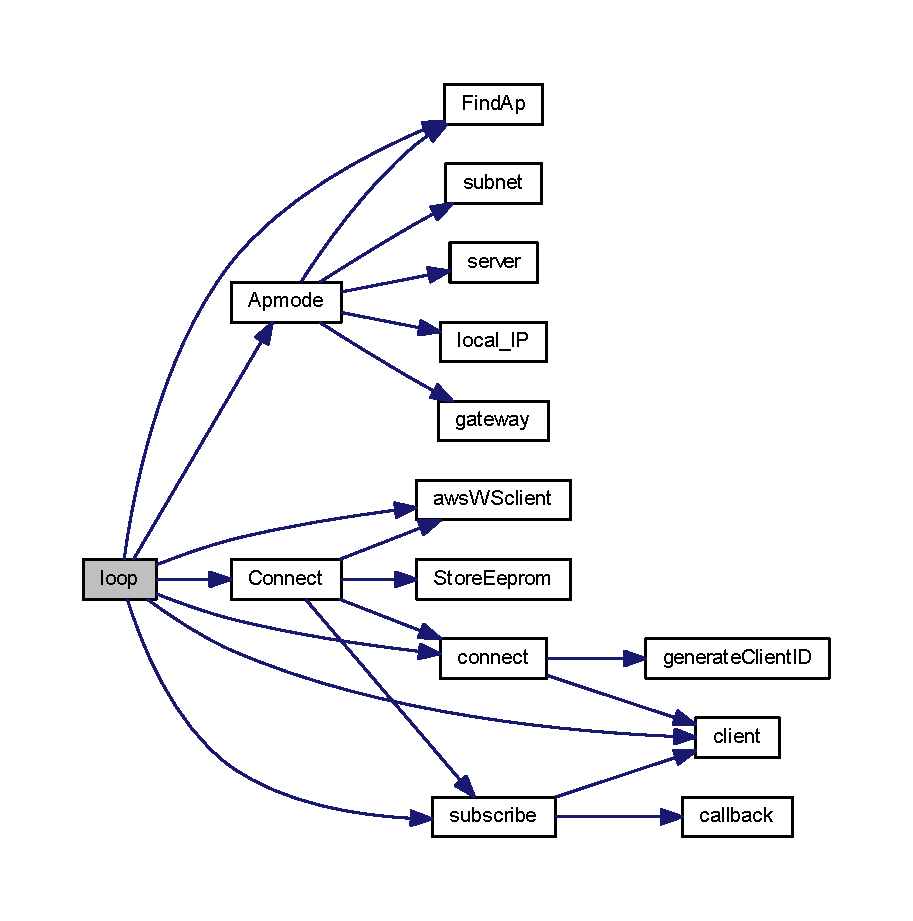
\includegraphics[width=350pt]{sl__uart__task_8c_afe461d27b9c48d5921c00d521181f12f_cgraph}
\end{center}
\end{figure}
\mbox{\Hypertarget{sl__uart__task_8c_a20ce1fcbc3f39da9ceaf09dbd5ca5ef8}\label{sl__uart__task_8c_a20ce1fcbc3f39da9ceaf09dbd5ca5ef8}} 
\index{sl\+\_\+uart\+\_\+task.\+c@{sl\+\_\+uart\+\_\+task.\+c}!responsecmd@{responsecmd}}
\index{responsecmd@{responsecmd}!sl\+\_\+uart\+\_\+task.\+c@{sl\+\_\+uart\+\_\+task.\+c}}
\subsubsection{\texorpdfstring{responsecmd()}{responsecmd()}}
{\footnotesize\ttfamily void responsecmd (\begin{DoxyParamCaption}\item[{char $\ast$}]{readcmd }\end{DoxyParamCaption})}



응답 데이터 형식지정 함수 

파라미터 readcmd의 데이터를 가지고 응답 데이터 형식을 만든다 \begin{DoxySeeAlso}{참고}
이 함수의 코드분석 내용
\begin{DoxyEnumerate}
\item wifi가 연결되어있다면 wifi의 감도에 따라 데이터 지정~\newline

\item wifi의 상태를 global 구조체 \mbox{\hyperlink{sl__uart__task_8c_a45bb259cfa999c850530718ccac5609b}{g\+\_\+\+Wall\+Pad}} 의 emode에 따라 지정~\newline

\item 파라미터 readcmd\mbox{[}0\mbox{]} (Header)에 따라 구조형식을 맞춘다 \mbox{[}참고 \+: 표\mbox{]}~\newline

\item 완성된 응답 데이터 형식의 체크섬을 값을 맨 마지막에 넣는다~\newline

\item 시리얼 통신으로 값을 보낸다~\newline

\item global 변수(int) msgsend값을 하나 줄인다 
\end{DoxyEnumerate}
\end{DoxySeeAlso}

\begin{DoxyParams}{매개변수}
{\em char} & $\ast$ readcmd \+: Wifi Module $>$ Wall Pad \\
\hline
\end{DoxyParams}
\begin{DoxyReturn}{반환값}
-\/ 
\end{DoxyReturn}


sl\+\_\+uart\+\_\+task.\+c 파일의 142 번째 라인에서 정의되었습니다.


\begin{DoxyCode}
142                                \{
143   \textcolor{comment}{// 통신 포맷 변경}
144   \textcolor{keywordflow}{if}(readcmd[0]== 0xc7)
145     \mbox{\hyperlink{sl__uart__task_8c_a0dc0281c6f27e62a5cb21cde5288a9a5}{DebugSerial}}.println(\textcolor{stringliteral}{"ERVcmd sended"});
146   \textcolor{keywordflow}{else} \textcolor{keywordflow}{if}(readcmd[0] == 0xc5)\{
147     \mbox{\hyperlink{sl__uart__task_8c_a0dc0281c6f27e62a5cb21cde5288a9a5}{DebugSerial}}.println(\textcolor{stringliteral}{"FCUcmd sended"});
148   \}
149 
150   \textcolor{comment}{// wifi 감도}
151   byte cmd[8];
152     \textcolor{keywordflow}{if}(WiFi.isConnected())\{
153       \textcolor{keywordflow}{if}(WiFi.RSSI() < - 85)\{
154         cmd[1] = 0x01;
155       \}
156       \textcolor{keywordflow}{else} \textcolor{keywordflow}{if}(WiFi.RSSI() < -75)\{
157         cmd[1] = 0x02;
158       \}
159       \textcolor{keywordflow}{else}\{
160         cmd[1] = 0x03;
161       \}
162     \}
163 
164   \textcolor{comment}{// wifi 상태}
165     \textcolor{keywordflow}{switch}(\mbox{\hyperlink{sl__uart__task_8c_a45bb259cfa999c850530718ccac5609b}{g\_WallPad}}.\mbox{\hyperlink{struct_st_wall_pad_a51f947b3c4ad6a33d096bfaf1caedb6e}{eMode}})\{
166         \textcolor{keywordflow}{case} \mbox{\hyperlink{_wall_pad_common_8h_a01baed20aab6218b9846cc7c935f8de9a1f5cc10773bdfbec3b85c915572c4d8d}{eMODE\_AP}}:\textcolor{keywordflow}{default}:
167           cmd[5] = 0x00; \textcolor{comment}{//WIFI status AP mode disconnected}
168         \textcolor{keywordflow}{break};
169         \textcolor{keywordflow}{case} \mbox{\hyperlink{_wall_pad_common_8h_a01baed20aab6218b9846cc7c935f8de9ae9734b024c572803a9131d2df41dece2}{eMODE\_CONNECT}}:
170             cmd[5] = 0x10; \textcolor{comment}{//WIFI status stand-alone mode disconnected}
171         \textcolor{keywordflow}{break};
172         \textcolor{keywordflow}{case} \mbox{\hyperlink{_wall_pad_common_8h_a01baed20aab6218b9846cc7c935f8de9a25a620c7255a0d3a02bf847826791ce2}{eMODE\_NORMAL}}:
173             cmd[5] = 0x11;
174         \textcolor{keywordflow}{break};   
175     \}
176 
177     \textcolor{keywordflow}{switch}(readcmd[0]) \{
178       \textcolor{comment}{// FCU : Wall pad 수신 : 상태/제어 응답}
179       \textcolor{keywordflow}{case} 0xa5 : \textcolor{keywordflow}{case} 0xb5:
180         cmd[0] = 0xd5;
181         cmd[2] = (byte)readcmd[2];  \textcolor{comment}{//MODE&FAN}
182         cmd[3] = (byte)readcmd[3];  \textcolor{comment}{//FLAG}
183         cmd[4] = (byte)readcmd[4];  \textcolor{comment}{//TARGET TEMP}
184         cmd[6] = 0x00;
185       \textcolor{keywordflow}{break};
186 
187       \textcolor{comment}{// FCU : Wall pad 수신 : Wifi 초기화 응답}
188       \textcolor{keywordflow}{case} 0xe5:
189         cmd[0] = 0xf5;
190         cmd[2] = 0x00;
191         cmd[3] = 0x00;
192         cmd[4] = 0x00;
193         cmd[6] = 0x00;
194         \mbox{\hyperlink{sl__uart__task_8c_a45bb259cfa999c850530718ccac5609b}{g\_WallPad}}.\mbox{\hyperlink{struct_st_wall_pad_a51f947b3c4ad6a33d096bfaf1caedb6e}{eMode}} = \mbox{\hyperlink{_wall_pad_common_8h_a01baed20aab6218b9846cc7c935f8de9a1f5cc10773bdfbec3b85c915572c4d8d}{eMODE\_AP}};
195         WiFi.mode(WIFI\_OFF);
196         strcpy( \mbox{\hyperlink{sl__uart__task_8c_a45bb259cfa999c850530718ccac5609b}{g\_WallPad}}.\mbox{\hyperlink{struct_st_wall_pad_afb1618185a1aecb8c77eff2f1453c24f}{sSsId}}     , \mbox{\hyperlink{sl__uart__task_8c_aa5d0ec846e4a5c3218b26ac91b89c137}{g\_sInitSsid}}   );
197         strcpy( \mbox{\hyperlink{sl__uart__task_8c_a45bb259cfa999c850530718ccac5609b}{g\_WallPad}}.\mbox{\hyperlink{struct_st_wall_pad_a8c77e9b61d65201646350d01f8a8d7c0}{sSsPass}}   , \mbox{\hyperlink{sl__uart__task_8c_a1bdc597aadbd6a0b8f8ddfdc4aee425e}{g\_sInitSspass}}   );
198       \textcolor{keywordflow}{break};
199 
200       \textcolor{comment}{// ERV : Wall Pad 수신 : 상태/제어 응답}
201       \textcolor{keywordflow}{case} 0xa7: \textcolor{keywordflow}{case} 0xb7: \textcolor{keywordflow}{case} 0xb8:
202         cmd[0] = 0xd7;
203         cmd[2] = (byte)readcmd[2];
204         cmd[3] = (byte)readcmd[3];
205         cmd[4] = (byte)readcmd[4];
206         cmd[6] = 0x00;
207       \textcolor{keywordflow}{break};
208 
209       \textcolor{keywordflow}{case} 0xc5: \textcolor{keywordflow}{case} 0xc7:
210         cmd[0] = (byte)readcmd[0];
211         cmd[2] = (byte)readcmd[2];
212         cmd[3] = (byte)readcmd[3];
213         cmd[4] = (byte)readcmd[4];
214         cmd[6] = 0x00;
215       \textcolor{keywordflow}{break};
216 
217     \}
218 
219     \textcolor{comment}{// CHECK SUM}
220     cmd[7] = cmd[0]^cmd[1]^cmd[2]^cmd[3]^cmd[4]^cmd[5]^cmd[6];
221 
222     \textcolor{keywordflow}{for}(\textcolor{keywordtype}{int} i = 0 ; i < 8 ; i++)
223     \{
224       Serial.write(cmd[i]);
225     \}
226     
227     \textcolor{keywordflow}{if}(\mbox{\hyperlink{sl__uart__task_8c_a9eaf86bfd30962df9aff407bd4840336}{g\_msgSend}}>0)\{
228       \mbox{\hyperlink{sl__uart__task_8c_a9eaf86bfd30962df9aff407bd4840336}{g\_msgSend}}--;
229     \}
230 \}
\end{DoxyCode}
이 함수를 호출하는 함수들에 대한 그래프입니다.\+:\nopagebreak
\begin{figure}[H]
\begin{center}
\leavevmode
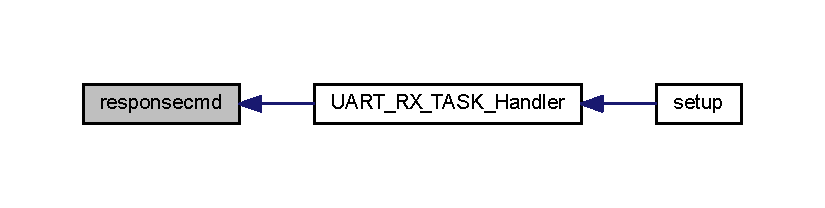
\includegraphics[width=350pt]{sl__uart__task_8c_a20ce1fcbc3f39da9ceaf09dbd5ca5ef8_icgraph}
\end{center}
\end{figure}
\mbox{\Hypertarget{sl__uart__task_8c_a8a2d61a985df99709d3d8c5ef7d46605}\label{sl__uart__task_8c_a8a2d61a985df99709d3d8c5ef7d46605}} 
\index{sl\+\_\+uart\+\_\+task.\+c@{sl\+\_\+uart\+\_\+task.\+c}!send\+Aws\+Msg@{send\+Aws\+Msg}}
\index{send\+Aws\+Msg@{send\+Aws\+Msg}!sl\+\_\+uart\+\_\+task.\+c@{sl\+\_\+uart\+\_\+task.\+c}}
\subsubsection{\texorpdfstring{send\+Aws\+Msg()}{sendAwsMsg()}\hspace{0.1cm}{\footnotesize\ttfamily [1/2]}}
{\footnotesize\ttfamily void send\+Aws\+Msg (\begin{DoxyParamCaption}\item[{char $\ast$}]{readcmd,  }\item[{bool}]{appstate }\end{DoxyParamCaption})}



publishing 함수 

파라미터 readcmd와 appstate 정보를 가지고 정보를 가공해 메세지를 보낸다 \begin{DoxySeeAlso}{참고}
이 함수의 코드분석 내용
\begin{DoxyEnumerate}
\item 파라미터 appstate 상태 확인~\newline

\item 파라미터 readcmd\mbox{[}0\mbox{]} (header)정보와 global 구조체 Last\+Send의 정보를 비교한다~\newline

\item 파라미터 readcmd\mbox{[}0\mbox{]} (header)정보가 F\+C\+U의 상태/제어 응답인 경우 \+: readcmd 정보를 가공해 버퍼에 저장하고 checksum값을 global 구조체 Last\+Send에 넣는다~\newline

\item 파라미터 readcmd\mbox{[}0\mbox{]} (header)정보가 E\+R\+V의 상태/제어 응답인 경우 \+: readcmd 정보를 가공해 버퍼에 저장하고 checksum값을 global 구조체 Last\+Send에 넣는다~\newline

\item 파라미터 readcmd\mbox{[}0\mbox{]} (header)정보가 그외 메시지인 경우 \+: readcmd 정보를 가공해 버퍼에 저장하고 checksum값을 global 구조체 Last\+Send에 넣는다~\newline

\item 현재 온도 정수 값을 global 구조체 Last\+Send에 넣는다~\newline

\item 가공된 버퍼를 지정된 topic에 publish한다~\newline

\item global 변수(bool) g\+\_\+b\+Appctl를 false로 대입한다 
\end{DoxyEnumerate}
\end{DoxySeeAlso}

\begin{DoxyParams}{매개변수}
{\em char} & $\ast$ readcmd \+: Wifi Module $<$ Wall Pad \\
\hline
{\em bool} & appstate \\
\hline
\end{DoxyParams}
\begin{DoxyReturn}{반환값}
-\/ 
\end{DoxyReturn}


sl\+\_\+uart\+\_\+task.\+c 파일의 355 번째 라인에서 정의되었습니다.


\begin{DoxyCode}
355                                                \{
356     \textcolor{comment}{//send a message   }
357     \textcolor{keywordtype}{char} buf[100];
358 
359     \textcolor{keywordflow}{if}(!appstate)\{
360       \textcolor{keywordflow}{if}(readcmd[0] == 0xb5 && (abs(\mbox{\hyperlink{sl__uart__task_8c_a9ee5ac74e0a6f3ba41e7bbcd03c316f4}{g\_LastSend}}.\mbox{\hyperlink{struct_st_last_send_a7ea4080d1f39154be7d7b1bfd6ff3987}{cTemp}} - readcmd[5]) < 1 ) || (
      \mbox{\hyperlink{sl__uart__task_8c_a9ee5ac74e0a6f3ba41e7bbcd03c316f4}{g\_LastSend}}.\mbox{\hyperlink{struct_st_last_send_ae99178f09a1a9fed4ba8f4603f165d17}{cFcu}} == readcmd[7]) ) \textcolor{keywordflow}{return};
361       \textcolor{keywordflow}{if}(readcmd[0] == 0xb7 && (abs(\mbox{\hyperlink{sl__uart__task_8c_a9ee5ac74e0a6f3ba41e7bbcd03c316f4}{g\_LastSend}}.\mbox{\hyperlink{struct_st_last_send_a7ea4080d1f39154be7d7b1bfd6ff3987}{cTemp}} - readcmd[5]) < 1 ) || (
      \mbox{\hyperlink{sl__uart__task_8c_a9ee5ac74e0a6f3ba41e7bbcd03c316f4}{g\_LastSend}}.\mbox{\hyperlink{struct_st_last_send_a47a441ff5eafccfc6171e25c5ea0c311}{cErv}} == readcmd[7]) )\textcolor{keywordflow}{return};
362       \textcolor{keywordflow}{if}(readcmd[0] == 0xb8 && (\mbox{\hyperlink{sl__uart__task_8c_a9ee5ac74e0a6f3ba41e7bbcd03c316f4}{g\_LastSend}}.\mbox{\hyperlink{struct_st_last_send_adaef2dbbc191c190520eab895effe14a}{cSensor}} == readcmd[7]) )\textcolor{keywordflow}{return};
363     \}
364     \textcolor{comment}{//FCU}
365     \textcolor{keywordflow}{if}(readcmd[0] == 0xb5 || readcmd[0] == 0xa5 )\{
366       sprintf(buf, \textcolor{stringliteral}{"\{\(\backslash\)"state\(\backslash\)":\{\(\backslash\)"reported\(\backslash\)":\{\(\backslash\)"cmd\(\backslash\)": [%d,%d,%d,%d,%d,%d,%d,%d]\}\}\}"}, readcmd[0], readcmd[1
      ],readcmd[2], readcmd[3],readcmd[4], readcmd[5],readcmd[6], readcmd[7]);
367       \mbox{\hyperlink{sl__uart__task_8c_a9ee5ac74e0a6f3ba41e7bbcd03c316f4}{g\_LastSend}}.\mbox{\hyperlink{struct_st_last_send_ae99178f09a1a9fed4ba8f4603f165d17}{cFcu}} = readcmd[7];
368     \}
369     \textcolor{comment}{//ERV}
370     \textcolor{keywordflow}{else} \textcolor{keywordflow}{if}(readcmd[0] == 0xb7 || readcmd[0] == 0xa7)\{ 
371       sprintf(buf, \textcolor{stringliteral}{"\{\(\backslash\)"state\(\backslash\)":\{\(\backslash\)"reported\(\backslash\)":\{\(\backslash\)"cmdERV\(\backslash\)": [%d,%d,%d,%d,%d,%d,%d,%d]\}\}\}"}, readcmd[0], 
      readcmd[1],readcmd[2], readcmd[3],readcmd[4], readcmd[5],readcmd[6], readcmd[7]);
372       \mbox{\hyperlink{sl__uart__task_8c_a9ee5ac74e0a6f3ba41e7bbcd03c316f4}{g\_LastSend}}.\mbox{\hyperlink{struct_st_last_send_a47a441ff5eafccfc6171e25c5ea0c311}{cErv}} = readcmd[7];
373     \}
374 
375     \textcolor{keywordflow}{else} \textcolor{keywordflow}{if}(readcmd[0] == 0xb8)\{
376       sprintf(buf, \textcolor{stringliteral}{"\{\(\backslash\)"state\(\backslash\)":\{\(\backslash\)"reported\(\backslash\)":\{\(\backslash\)"sensorState\(\backslash\)": [%d,%d,%d,%d,%d,%d,%d,%d]\}\}\}"}, readcmd[0], 
      readcmd[1],readcmd[2], readcmd[3],readcmd[4], readcmd[5],readcmd[6], readcmd[7]);
377       \mbox{\hyperlink{sl__uart__task_8c_a9ee5ac74e0a6f3ba41e7bbcd03c316f4}{g\_LastSend}}.\mbox{\hyperlink{struct_st_last_send_adaef2dbbc191c190520eab895effe14a}{cSensor}} = readcmd[7];
378     \}
379   
380     \mbox{\hyperlink{sl__uart__task_8c_a9ee5ac74e0a6f3ba41e7bbcd03c316f4}{g\_LastSend}}.\mbox{\hyperlink{struct_st_last_send_a7ea4080d1f39154be7d7b1bfd6ff3987}{cTemp}} = readcmd[5];
381     \textcolor{keywordtype}{int} rc = \mbox{\hyperlink{sl__uart__task_8c_aed38f3e7ee0565ea6703f91a12983f54}{client}}.publish(\mbox{\hyperlink{sl__uart__task_8c_af0a4f1814f6df77902506d568db1b886}{aws\_topic\_update}}, buf);
382     \mbox{\hyperlink{sl__uart__task_8c_a06be4e59ee6e13a5f54dba4c3f014ec5}{g\_bAppctl}} = \textcolor{keyword}{false};
383 \}
\end{DoxyCode}
이 함수 내부에서 호출하는 함수들에 대한 그래프입니다.\+:\nopagebreak
\begin{figure}[H]
\begin{center}
\leavevmode
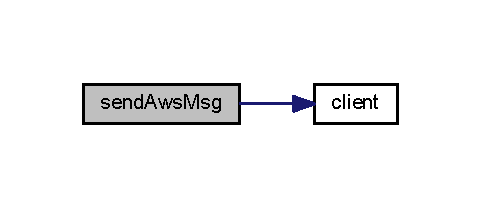
\includegraphics[width=231pt]{sl__uart__task_8c_a8a2d61a985df99709d3d8c5ef7d46605_cgraph}
\end{center}
\end{figure}
이 함수를 호출하는 함수들에 대한 그래프입니다.\+:\nopagebreak
\begin{figure}[H]
\begin{center}
\leavevmode
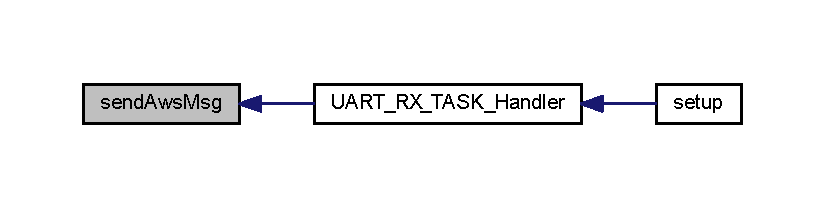
\includegraphics[width=350pt]{sl__uart__task_8c_a8a2d61a985df99709d3d8c5ef7d46605_icgraph}
\end{center}
\end{figure}
\mbox{\Hypertarget{sl__uart__task_8c_aac99a2341cbcfcbd24f7aba50e2ff771}\label{sl__uart__task_8c_aac99a2341cbcfcbd24f7aba50e2ff771}} 
\index{sl\+\_\+uart\+\_\+task.\+c@{sl\+\_\+uart\+\_\+task.\+c}!send\+Aws\+Msg@{send\+Aws\+Msg}}
\index{send\+Aws\+Msg@{send\+Aws\+Msg}!sl\+\_\+uart\+\_\+task.\+c@{sl\+\_\+uart\+\_\+task.\+c}}
\subsubsection{\texorpdfstring{send\+Aws\+Msg()}{sendAwsMsg()}\hspace{0.1cm}{\footnotesize\ttfamily [2/2]}}
{\footnotesize\ttfamily void send\+Aws\+Msg (\begin{DoxyParamCaption}\item[{char $\ast$}]{readcmd }\end{DoxyParamCaption})}

\mbox{\Hypertarget{sl__uart__task_8c_a5042d50338e981034cfb61c6067ab043}\label{sl__uart__task_8c_a5042d50338e981034cfb61c6067ab043}} 
\index{sl\+\_\+uart\+\_\+task.\+c@{sl\+\_\+uart\+\_\+task.\+c}!server@{server}}
\index{server@{server}!sl\+\_\+uart\+\_\+task.\+c@{sl\+\_\+uart\+\_\+task.\+c}}
\subsubsection{\texorpdfstring{server()}{server()}}
{\footnotesize\ttfamily Wi\+Fi\+Server server (\begin{DoxyParamCaption}\item[{30300}]{ }\end{DoxyParamCaption})}

이 함수를 호출하는 함수들에 대한 그래프입니다.\+:\nopagebreak
\begin{figure}[H]
\begin{center}
\leavevmode
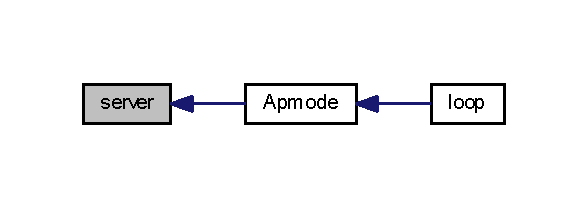
\includegraphics[width=282pt]{sl__uart__task_8c_a5042d50338e981034cfb61c6067ab043_icgraph}
\end{center}
\end{figure}
\mbox{\Hypertarget{sl__uart__task_8c_a4fc01d736fe50cf5b977f755b675f11d}\label{sl__uart__task_8c_a4fc01d736fe50cf5b977f755b675f11d}} 
\index{sl\+\_\+uart\+\_\+task.\+c@{sl\+\_\+uart\+\_\+task.\+c}!setup@{setup}}
\index{setup@{setup}!sl\+\_\+uart\+\_\+task.\+c@{sl\+\_\+uart\+\_\+task.\+c}}
\subsubsection{\texorpdfstring{setup()}{setup()}}
{\footnotesize\ttfamily void setup (\begin{DoxyParamCaption}{ }\end{DoxyParamCaption})}



task 설정 함수 

U\+A\+RT 통신을 위한 Baud rate와 E\+E\+P\+R\+OM 크기, system task관한 설정한다 \begin{DoxySeeAlso}{참고}
이 함수의 코드분석 내용
\begin{DoxyEnumerate}
\item wifi sleep 모드는 사용 안한다~\newline

\item U\+A\+RT 통신을 위한 Baud rate는 9600으로 한다~\newline

\item E\+E\+P\+R\+OM 크기를 구조체 \mbox{\hyperlink{_wall_pad_common_8h_afc78910c4749fa1230e1149115f9d70a}{Wall\+Pad}} 만큼한다~\newline

\item E\+E\+P\+R\+OM 체크 함수 호출한다~\newline

\item system\+\_\+os\+\_\+task A\+P\+I함수 \+: set up tasks~\newline
 bool system\+\_\+os\+\_\+task(os\+\_\+task\+\_\+t task, uint8 prio, os\+\_\+event\+\_\+t $\ast$queue, uint8 qlen)~\newline
 os\+\_\+task\+\_\+t task \+: task 함수~\newline
 uint8 prio \+: task 우선순위~\newline
 os\+\_\+event\+\_\+t $\ast$queue \+: 메세지 큐 포인터~\newline
 uint8 qlen \+: 메시지 큐 길이~\newline

\item os\+\_\+timer\+\_\+setfn A\+P\+I함수 \+: set timer \mbox{\hyperlink{sl__uart__task_8c_ac3a129f66dc859e2b7279565f4e1de78}{callback}} 함수~\newline
 oid os\+\_\+timer\+\_\+setfn (os\+\_\+timer\+\_\+t $\ast$ptimer, os\+\_\+timer\+\_\+func\+\_\+t $\ast$pfunction, void $\ast$parg)~\newline
 os\+\_\+timer\+\_\+t $\ast$ptimer \+: 타이머 구조체~\newline
 os\+\_\+timer\+\_\+func\+\_\+t $\ast$pfunction \+: timer \mbox{\hyperlink{sl__uart__task_8c_ac3a129f66dc859e2b7279565f4e1de78}{callback}} 함수~\newline
 void $\ast$parg \+: \mbox{\hyperlink{sl__uart__task_8c_ac3a129f66dc859e2b7279565f4e1de78}{callback}} 함수 파라미터~\newline

\item Temp\+\_\+\+Run\+\_\+\+U\+A\+R\+T\+\_\+\+R\+X\+\_\+\+Task(0) 함수를 호출한다~\newline

\item g\+\_\+\+Wall\+Pad의 e\+Mode값을 e\+M\+O\+D\+E\+\_\+\+N\+O\+N\+E로 변환한다~\newline

\end{DoxyEnumerate}
\end{DoxySeeAlso}

\begin{DoxyParams}{매개변수}
{\em -\/} & \\
\hline
\end{DoxyParams}
\begin{DoxyReturn}{반환값}
-\/ 
\end{DoxyReturn}


sl\+\_\+uart\+\_\+task.\+c 파일의 1022 번째 라인에서 정의되었습니다.


\begin{DoxyCode}
1022              \{
1023   wifi\_set\_sleep\_type(NONE\_SLEEP\_T);
1024 
1025   
1026   \mbox{\hyperlink{sl__uart__task_8c_a161f66c89721d6e10e0f626e305c6013}{WallpadSerial}}.begin(9600);
1027   \mbox{\hyperlink{sl__uart__task_8c_a0dc0281c6f27e62a5cb21cde5288a9a5}{DebugSerial}}.begin(115200);
1028   
1029   \mbox{\hyperlink{sl__uart__task_8c_a0dc0281c6f27e62a5cb21cde5288a9a5}{DebugSerial}}.setDebugOutput(\textcolor{keyword}{true});
1030   \mbox{\hyperlink{sl__uart__task_8c_a0dc0281c6f27e62a5cb21cde5288a9a5}{DebugSerial}}.setTimeout(10);
1031 
1032   EEPROM.begin(\textcolor{keyword}{sizeof}(\mbox{\hyperlink{struct_st_wall_pad}{WallPad}}));
1033   \mbox{\hyperlink{sl__uart__task_8c_ac4dd7f628ac36ff312d47a898d0573d6}{CheckEeprom}}();
1034 
1035   \textcolor{comment}{//thread olusturma}
1036   system\_os\_task(\mbox{\hyperlink{sl__uart__task_8c_a35bd387bc89edc5110da50f77d737813}{UART\_RX\_TASK\_Handler}},
1037     \mbox{\hyperlink{sl__uart__task_8c_aca8e8e20d2136c68476203baa1ee3029}{UART\_RX\_TASK\_PRIORITY}}, \mbox{\hyperlink{sl__uart__task_8c_aa67c702a9e31bd1b512f4ac8b152c65d}{UART\_RX\_QUEUE}},
1038     \mbox{\hyperlink{sl__uart__task_8c_a6a9f5253345bffef8276cc5070177572}{UART\_RX\_QUEUE\_SIZE}});
1039 
1040   \textcolor{comment}{//timer olusturma}
1041   os\_timer\_setfn(&\mbox{\hyperlink{sl__uart__task_8c_aaab2b2dd61c91cddbaa9e130d26d5dce}{UART\_RX\_TASK\_Timer}}, 
1042       (os\_timer\_func\_t*)&\mbox{\hyperlink{sl__uart__task_8c_a93049dd8aee54bb4e745e526542c36f7}{Temp\_Run\_UART\_RX\_Task}}, 0);
1043 
1044   \textcolor{comment}{//taski baslatma}
1045   \mbox{\hyperlink{sl__uart__task_8c_a93049dd8aee54bb4e745e526542c36f7}{Temp\_Run\_UART\_RX\_Task}}(0);
1046     
1047     \mbox{\hyperlink{sl__uart__task_8c_a45bb259cfa999c850530718ccac5609b}{g\_WallPad}}.\mbox{\hyperlink{struct_st_wall_pad_a51f947b3c4ad6a33d096bfaf1caedb6e}{eMode}} = \mbox{\hyperlink{_wall_pad_common_8h_a01baed20aab6218b9846cc7c935f8de9abb51c808160be71ef81bc5880610bedc}{eMODE\_NONE}};
1048 
1049 \}
\end{DoxyCode}
이 함수 내부에서 호출하는 함수들에 대한 그래프입니다.\+:\nopagebreak
\begin{figure}[H]
\begin{center}
\leavevmode
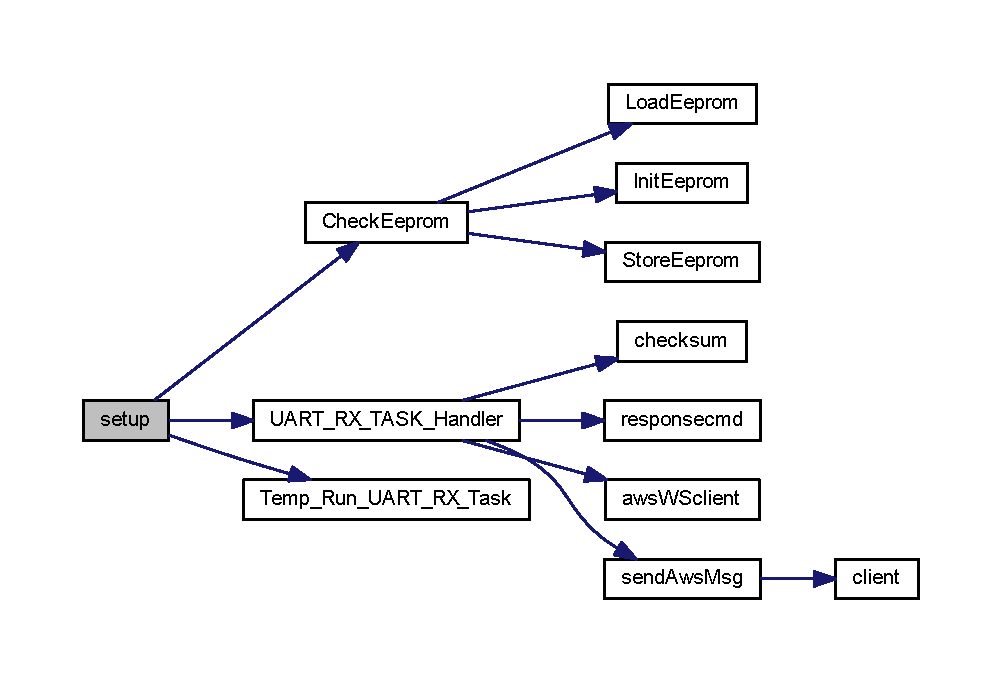
\includegraphics[width=350pt]{sl__uart__task_8c_a4fc01d736fe50cf5b977f755b675f11d_cgraph}
\end{center}
\end{figure}
\mbox{\Hypertarget{sl__uart__task_8c_a77d6a883c5cf0c92dcc225685249e38e}\label{sl__uart__task_8c_a77d6a883c5cf0c92dcc225685249e38e}} 
\index{sl\+\_\+uart\+\_\+task.\+c@{sl\+\_\+uart\+\_\+task.\+c}!Store\+Eeprom@{Store\+Eeprom}}
\index{Store\+Eeprom@{Store\+Eeprom}!sl\+\_\+uart\+\_\+task.\+c@{sl\+\_\+uart\+\_\+task.\+c}}
\subsubsection{\texorpdfstring{Store\+Eeprom()}{StoreEeprom()}}
{\footnotesize\ttfamily void Store\+Eeprom (\begin{DoxyParamCaption}\item[{void}]{ }\end{DoxyParamCaption})}



E\+E\+P\+R\+OM 쓰기 함수 

global 구조체 g\+\_\+\+Wall\+Pad 값을 E\+E\+P\+R\+O\+M에 세팅한다 \begin{DoxySeeAlso}{참고}
이 함수의 코드분석 내용
\begin{DoxyEnumerate}
\item global 구조체 g\+\_\+\+Wall\+Pad를 포인터로 연결한다~\newline

\item global 구조체 \mbox{\hyperlink{sl__uart__task_8c_a45bb259cfa999c850530718ccac5609b}{g\+\_\+\+Wall\+Pad}} 크기만큼 E\+E\+P\+R\+O\+M를 global 구조체 \mbox{\hyperlink{sl__uart__task_8c_a45bb259cfa999c850530718ccac5609b}{g\+\_\+\+Wall\+Pad}} 값으로 세팅한다 
\end{DoxyEnumerate}
\end{DoxySeeAlso}

\begin{DoxyParams}{매개변수}
{\em -\/} & \\
\hline
\end{DoxyParams}
\begin{DoxyReturn}{반환값}
-\/ 
\end{DoxyReturn}


sl\+\_\+uart\+\_\+task.\+c 파일의 616 번째 라인에서 정의되었습니다.


\begin{DoxyCode}
617 \{
618    \textcolor{keywordtype}{char}* pSetData = ( \textcolor{keywordtype}{char}*) &\mbox{\hyperlink{sl__uart__task_8c_a45bb259cfa999c850530718ccac5609b}{g\_WallPad}};
619   \textcolor{keywordtype}{int} i;
620   \textcolor{keywordflow}{for}( i=0; i < \textcolor{keyword}{sizeof}( \mbox{\hyperlink{_wall_pad_common_8h_afc78910c4749fa1230e1149115f9d70a}{WallPad}} ); i++ )
621     EEPROM.write( i, *pSetData++ );
622   EEPROM.commit();
623 \}
\end{DoxyCode}
이 함수를 호출하는 함수들에 대한 그래프입니다.\+:\nopagebreak
\begin{figure}[H]
\begin{center}
\leavevmode
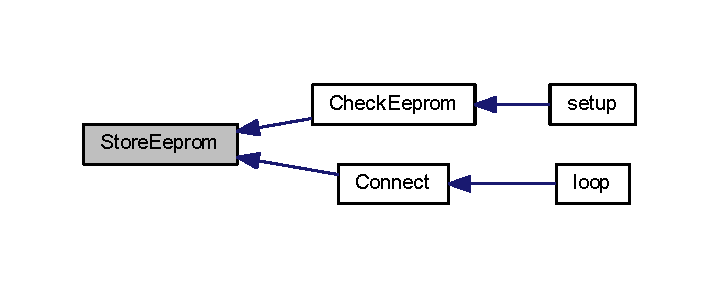
\includegraphics[width=345pt]{sl__uart__task_8c_a77d6a883c5cf0c92dcc225685249e38e_icgraph}
\end{center}
\end{figure}
\mbox{\Hypertarget{sl__uart__task_8c_a89cf134ada28d8ce0192d9fcbc83614a}\label{sl__uart__task_8c_a89cf134ada28d8ce0192d9fcbc83614a}} 
\index{sl\+\_\+uart\+\_\+task.\+c@{sl\+\_\+uart\+\_\+task.\+c}!subnet@{subnet}}
\index{subnet@{subnet}!sl\+\_\+uart\+\_\+task.\+c@{sl\+\_\+uart\+\_\+task.\+c}}
\subsubsection{\texorpdfstring{subnet()}{subnet()}}
{\footnotesize\ttfamily I\+P\+Address subnet (\begin{DoxyParamCaption}\item[{255}]{,  }\item[{255}]{,  }\item[{255}]{,  }\item[{0}]{ }\end{DoxyParamCaption})}

이 함수를 호출하는 함수들에 대한 그래프입니다.\+:\nopagebreak
\begin{figure}[H]
\begin{center}
\leavevmode
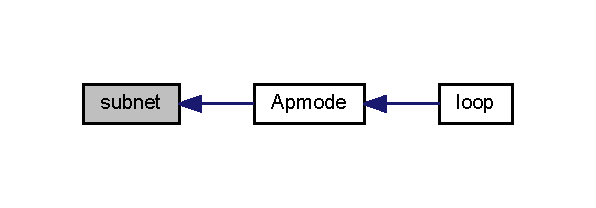
\includegraphics[width=286pt]{sl__uart__task_8c_a89cf134ada28d8ce0192d9fcbc83614a_icgraph}
\end{center}
\end{figure}
\mbox{\Hypertarget{sl__uart__task_8c_a0bccd94c4239c019c480e507cb6159ee}\label{sl__uart__task_8c_a0bccd94c4239c019c480e507cb6159ee}} 
\index{sl\+\_\+uart\+\_\+task.\+c@{sl\+\_\+uart\+\_\+task.\+c}!subscribe@{subscribe}}
\index{subscribe@{subscribe}!sl\+\_\+uart\+\_\+task.\+c@{sl\+\_\+uart\+\_\+task.\+c}}
\subsubsection{\texorpdfstring{subscribe()}{subscribe()}}
{\footnotesize\ttfamily void subscribe (\begin{DoxyParamCaption}{ }\end{DoxyParamCaption})}



M\+Q\+TT subscribe 함수 

client callback함수와 M\+Q\+TT topic을 지정한다 
\begin{DoxyParams}{매개변수}
{\em -\/} & \\
\hline
\end{DoxyParams}
\begin{DoxyReturn}{반환값}
-\/ 
\end{DoxyReturn}


sl\+\_\+uart\+\_\+task.\+c 파일의 327 번째 라인에서 정의되었습니다.


\begin{DoxyCode}
327                   \{
328     \mbox{\hyperlink{sl__uart__task_8c_aed38f3e7ee0565ea6703f91a12983f54}{client}}.setCallback(\mbox{\hyperlink{sl__uart__task_8c_ac3a129f66dc859e2b7279565f4e1de78}{callback}});
329     \mbox{\hyperlink{sl__uart__task_8c_aed38f3e7ee0565ea6703f91a12983f54}{client}}.subscribe(\mbox{\hyperlink{sl__uart__task_8c_a1bffe679a4beca9eb4d24e8a6d72ec8a}{aws\_topic}});
330 
331    \textcolor{comment}{//subscript to a topic}
332     \mbox{\hyperlink{sl__uart__task_8c_a0dc0281c6f27e62a5cb21cde5288a9a5}{DebugSerial}}.println(\textcolor{stringliteral}{"MQTT subscribed"});
333 \}
\end{DoxyCode}
이 함수 내부에서 호출하는 함수들에 대한 그래프입니다.\+:\nopagebreak
\begin{figure}[H]
\begin{center}
\leavevmode
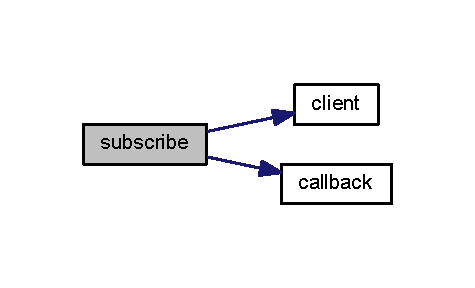
\includegraphics[width=228pt]{sl__uart__task_8c_a0bccd94c4239c019c480e507cb6159ee_cgraph}
\end{center}
\end{figure}
이 함수를 호출하는 함수들에 대한 그래프입니다.\+:\nopagebreak
\begin{figure}[H]
\begin{center}
\leavevmode
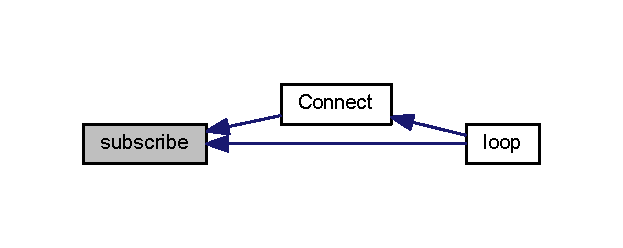
\includegraphics[width=299pt]{sl__uart__task_8c_a0bccd94c4239c019c480e507cb6159ee_icgraph}
\end{center}
\end{figure}
\mbox{\Hypertarget{sl__uart__task_8c_a93049dd8aee54bb4e745e526542c36f7}\label{sl__uart__task_8c_a93049dd8aee54bb4e745e526542c36f7}} 
\index{sl\+\_\+uart\+\_\+task.\+c@{sl\+\_\+uart\+\_\+task.\+c}!Temp\+\_\+\+Run\+\_\+\+U\+A\+R\+T\+\_\+\+R\+X\+\_\+\+Task@{Temp\+\_\+\+Run\+\_\+\+U\+A\+R\+T\+\_\+\+R\+X\+\_\+\+Task}}
\index{Temp\+\_\+\+Run\+\_\+\+U\+A\+R\+T\+\_\+\+R\+X\+\_\+\+Task@{Temp\+\_\+\+Run\+\_\+\+U\+A\+R\+T\+\_\+\+R\+X\+\_\+\+Task}!sl\+\_\+uart\+\_\+task.\+c@{sl\+\_\+uart\+\_\+task.\+c}}
\subsubsection{\texorpdfstring{Temp\+\_\+\+Run\+\_\+\+U\+A\+R\+T\+\_\+\+R\+X\+\_\+\+Task()}{Temp\_Run\_UART\_RX\_Task()}}
{\footnotesize\ttfamily void Temp\+\_\+\+Run\+\_\+\+U\+A\+R\+T\+\_\+\+R\+X\+\_\+\+Task (\begin{DoxyParamCaption}\item[{void $\ast$}]{ }\end{DoxyParamCaption})}



task 메세지를 보내는 함수 

E\+S\+P8266 N\+On-\/os S\+D\+K에서 제공되는 A\+P\+I를 호출하는 함수~\newline
 이 함수 내부의 system\+\_\+os\+\_\+post함수를 지정된 형식으로 호출된다 (E\+S\+P8266-\/\+U\+A\+R\+T-\/\+R\+X-\/\+Interrupt) \begin{DoxySeeAlso}{참고}
이 함수의 코드분석 내용 system\+\_\+os\+\_\+post A\+P\+I함수만 살펴보면 된다~\newline
bool system\+\_\+os\+\_\+post (uint8 prio, os\+\_\+signal\+\_\+t sig, os\+\_\+param\+\_\+t par)~\newline
uint8 prio \+: task priority~\newline
os\+\_\+signal\+\_\+t sig \+: message type~\newline
os\+\_\+param\+\_\+t par \+: message parameters~\newline
여기서는 system\+\_\+os\+\_\+post(\+U\+A\+R\+T\+\_\+\+R\+X\+\_\+\+T\+A\+S\+K\+\_\+\+P\+R\+I\+O\+R\+I\+T\+Y, 0, 0)으로 사용했다~\newline
\mbox{\hyperlink{sl__uart__task_8c_aca8e8e20d2136c68476203baa1ee3029}{U\+A\+R\+T\+\_\+\+R\+X\+\_\+\+T\+A\+S\+K\+\_\+\+P\+R\+I\+O\+R\+I\+TY}} 값은 1이다 
\end{DoxySeeAlso}

\begin{DoxyParams}{매개변수}
{\em -\/} & \\
\hline
\end{DoxyParams}
\begin{DoxyReturn}{반환값}
-\/ 
\end{DoxyReturn}


sl\+\_\+uart\+\_\+task.\+c 파일의 520 번째 라인에서 정의되었습니다.


\begin{DoxyCode}
520                                   \{
521   system\_os\_post(\mbox{\hyperlink{sl__uart__task_8c_aca8e8e20d2136c68476203baa1ee3029}{UART\_RX\_TASK\_PRIORITY}}, 0, 0);
522 \}
\end{DoxyCode}
이 함수를 호출하는 함수들에 대한 그래프입니다.\+:\nopagebreak
\begin{figure}[H]
\begin{center}
\leavevmode
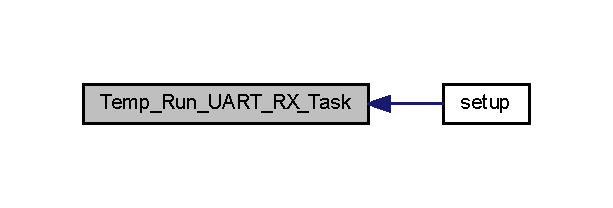
\includegraphics[width=294pt]{sl__uart__task_8c_a93049dd8aee54bb4e745e526542c36f7_icgraph}
\end{center}
\end{figure}
\mbox{\Hypertarget{sl__uart__task_8c_a35bd387bc89edc5110da50f77d737813}\label{sl__uart__task_8c_a35bd387bc89edc5110da50f77d737813}} 
\index{sl\+\_\+uart\+\_\+task.\+c@{sl\+\_\+uart\+\_\+task.\+c}!U\+A\+R\+T\+\_\+\+R\+X\+\_\+\+T\+A\+S\+K\+\_\+\+Handler@{U\+A\+R\+T\+\_\+\+R\+X\+\_\+\+T\+A\+S\+K\+\_\+\+Handler}}
\index{U\+A\+R\+T\+\_\+\+R\+X\+\_\+\+T\+A\+S\+K\+\_\+\+Handler@{U\+A\+R\+T\+\_\+\+R\+X\+\_\+\+T\+A\+S\+K\+\_\+\+Handler}!sl\+\_\+uart\+\_\+task.\+c@{sl\+\_\+uart\+\_\+task.\+c}}
\subsubsection{\texorpdfstring{U\+A\+R\+T\+\_\+\+R\+X\+\_\+\+T\+A\+S\+K\+\_\+\+Handler()}{UART\_RX\_TASK\_Handler()}}
{\footnotesize\ttfamily void U\+A\+R\+T\+\_\+\+R\+X\+\_\+\+T\+A\+S\+K\+\_\+\+Handler (\begin{DoxyParamCaption}\item[{os\+\_\+event\+\_\+t $\ast$}]{ }\end{DoxyParamCaption})}



U\+A\+R\+T\+\_\+\+R\+X\+\_\+\+T\+A\+S\+K\+\_\+\+Handler함수 (트랩) 

U\+A\+R\+T로 받은 데이터가 있는 확인 후 그 데이터를 경우따라 분류 후 타이머를 설정한다 \begin{DoxySeeAlso}{참고}
이 함수의 코드분석 내용
\begin{DoxyEnumerate}
\item 받은 데이터를 있는지 확인한다~\newline

\item 받은 데이터를 버퍼에 저장한다~\newline

\item global 변수(int) \mbox{\hyperlink{sl__uart__task_8c_a9eaf86bfd30962df9aff407bd4840336}{g\+\_\+msg\+Send}} 값이 0일 경우, 오류 확인 함수(checksum)로 버퍼의 값를 확인한다~\newline

\item 오류 시, 응답 데이터 형식지정 함수을 호출한다~\newline

\item wifi와 서버에 둘다 연결이 되어 있는 경우, publishing 함수를 호출한다~\newline

\item global 변수(int) \mbox{\hyperlink{sl__uart__task_8c_a9eaf86bfd30962df9aff407bd4840336}{g\+\_\+msg\+Send}} 값이 0이 아닐 경우, 응답 데이터 형식지정 함수을 호출한다~\newline

\item A\+P\+I함수인 os\+\_\+timer\+\_\+arm를 호출한다 (밀리초 타이머를 설정)~\newline
 void os\+\_\+timer\+\_\+arm (os\+\_\+timer\+\_\+t $\ast$ptimer, uint32\+\_\+t milliseconds, bool repeat\+\_\+flag)~\newline
 os\+\_\+timer\+\_\+t $\ast$ptimer \+: 타이머 구조체~\newline
 uinit32\+\_\+t milliseconds \+: ms~\newline
 bool repeat\+\_\+flag \+: 반복 유/무 설정 
\end{DoxyEnumerate}
\end{DoxySeeAlso}

\begin{DoxyParams}{매개변수}
{\em os\+\_\+event\+\_\+t$\ast$} & \\
\hline
\end{DoxyParams}
\begin{DoxyReturn}{반환값}
-\/ 
\end{DoxyReturn}


sl\+\_\+uart\+\_\+task.\+c 파일의 546 번째 라인에서 정의되었습니다.


\begin{DoxyCode}
546                                         \{
547 
548   \textcolor{comment}{/* Wallpad Serial RX buffer 점검}
549 \textcolor{comment}{   * if Wallpad Serial RX buffer is empty ==> WallpadSerial.available() return 0}
550 \textcolor{comment}{   * if something is filled in Wallpad Serial RX buffer  ==> WallpadSerial.available() return 1}
551 \textcolor{comment}{   */}
552   \textcolor{keywordflow}{if} (\mbox{\hyperlink{sl__uart__task_8c_a161f66c89721d6e10e0f626e305c6013}{WallpadSerial}}.available() > 0)
553   \{
554 
555     
556     \textcolor{comment}{//Wallpad로부터 8byte cmd 수신}
557     byte buf[8];
558     \mbox{\hyperlink{sl__uart__task_8c_a161f66c89721d6e10e0f626e305c6013}{WallpadSerial}}.readBytes(buf,8);
559 
560     \textcolor{keywordflow}{if}(!\mbox{\hyperlink{sl__uart__task_8c_a9eaf86bfd30962df9aff407bd4840336}{g\_msgSend}})\{
561       \textcolor{keywordflow}{if}(\mbox{\hyperlink{sl__uart__task_8c_a38f7f9361dece3c36092a307f845f0a6}{checksum}}((\textcolor{keywordtype}{char}*)buf))
562         \mbox{\hyperlink{sl__uart__task_8c_a20ce1fcbc3f39da9ceaf09dbd5ca5ef8}{responsecmd}}((\textcolor{keywordtype}{char}*)buf);
563         
564       \textcolor{comment}{//if (WiFi.isConnected() && awsWSclient.connected ()) \{      }
565       \textcolor{keywordflow}{if} (WiFi.isConnected() && \mbox{\hyperlink{sl__uart__task_8c_af273a6e233df1fa0ded638e07843b468}{awsWSclient}}.connected ()) \{    
566         \mbox{\hyperlink{sl__uart__task_8c_a8a2d61a985df99709d3d8c5ef7d46605}{sendAwsMsg}}((\textcolor{keywordtype}{char}*)buf , \mbox{\hyperlink{sl__uart__task_8c_a06be4e59ee6e13a5f54dba4c3f014ec5}{g\_bAppctl}});    
567       \}    
568       
569     \}
570 
571     \textcolor{keywordflow}{else}\{
572       \mbox{\hyperlink{sl__uart__task_8c_a20ce1fcbc3f39da9ceaf09dbd5ca5ef8}{responsecmd}}(\mbox{\hyperlink{sl__uart__task_8c_a073128b0e46bc8edcc1b5ea52715bddd}{g\_cmd}});
573     \}
574     
575   \}
576   
577   os\_timer\_arm(&\mbox{\hyperlink{sl__uart__task_8c_aaab2b2dd61c91cddbaa9e130d26d5dce}{UART\_RX\_TASK\_Timer}}, \mbox{\hyperlink{sl__uart__task_8c_a36baaeb855e27ca3d67e6e3e0230e974}{UART\_RX\_CYCLE\_IN\_MS}} \textcolor{comment}{/*ms*/}, 0 \textcolor{comment}{/*
      once*/});
578 \}
\end{DoxyCode}
이 함수 내부에서 호출하는 함수들에 대한 그래프입니다.\+:\nopagebreak
\begin{figure}[H]
\begin{center}
\leavevmode
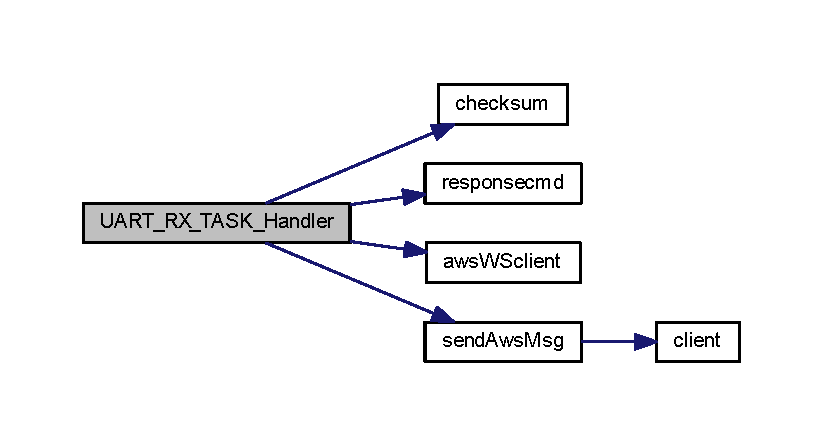
\includegraphics[width=350pt]{sl__uart__task_8c_a35bd387bc89edc5110da50f77d737813_cgraph}
\end{center}
\end{figure}
이 함수를 호출하는 함수들에 대한 그래프입니다.\+:\nopagebreak
\begin{figure}[H]
\begin{center}
\leavevmode
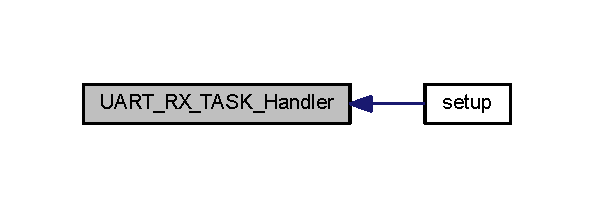
\includegraphics[width=285pt]{sl__uart__task_8c_a35bd387bc89edc5110da50f77d737813_icgraph}
\end{center}
\end{figure}


\subsection{변수 문서화}
\mbox{\Hypertarget{sl__uart__task_8c_a0977a0891557a2a5f83b635e5eb3443e}\label{sl__uart__task_8c_a0977a0891557a2a5f83b635e5eb3443e}} 
\index{sl\+\_\+uart\+\_\+task.\+c@{sl\+\_\+uart\+\_\+task.\+c}!aws\+\_\+endpoint@{aws\+\_\+endpoint}}
\index{aws\+\_\+endpoint@{aws\+\_\+endpoint}!sl\+\_\+uart\+\_\+task.\+c@{sl\+\_\+uart\+\_\+task.\+c}}
\subsubsection{\texorpdfstring{aws\+\_\+endpoint}{aws\_endpoint}}
{\footnotesize\ttfamily char aws\+\_\+endpoint\mbox{[}$\,$\mbox{]} = \char`\"{}a2q36qubve1ukk.\+iot.\+ap-\/northeast-\/2.amazonaws.\+com\char`\"{}}



sl\+\_\+uart\+\_\+task.\+c 파일의 240 번째 라인에서 정의되었습니다.

\mbox{\Hypertarget{sl__uart__task_8c_a45bf1e976b70d29f3c109c37a3b01b88}\label{sl__uart__task_8c_a45bf1e976b70d29f3c109c37a3b01b88}} 
\index{sl\+\_\+uart\+\_\+task.\+c@{sl\+\_\+uart\+\_\+task.\+c}!aws\+\_\+key@{aws\+\_\+key}}
\index{aws\+\_\+key@{aws\+\_\+key}!sl\+\_\+uart\+\_\+task.\+c@{sl\+\_\+uart\+\_\+task.\+c}}
\subsubsection{\texorpdfstring{aws\+\_\+key}{aws\_key}}
{\footnotesize\ttfamily char aws\+\_\+key\mbox{[}$\,$\mbox{]} = \char`\"{}A\+K\+I\+A\+J\+A4\+X53\+V\+A\+F\+T\+G\+E\+D\+Q3Q\char`\"{}}



sl\+\_\+uart\+\_\+task.\+c 파일의 241 번째 라인에서 정의되었습니다.

\mbox{\Hypertarget{sl__uart__task_8c_a3c3e0be700ab12b748d8c833ee2255a1}\label{sl__uart__task_8c_a3c3e0be700ab12b748d8c833ee2255a1}} 
\index{sl\+\_\+uart\+\_\+task.\+c@{sl\+\_\+uart\+\_\+task.\+c}!aws\+\_\+region@{aws\+\_\+region}}
\index{aws\+\_\+region@{aws\+\_\+region}!sl\+\_\+uart\+\_\+task.\+c@{sl\+\_\+uart\+\_\+task.\+c}}
\subsubsection{\texorpdfstring{aws\+\_\+region}{aws\_region}}
{\footnotesize\ttfamily char aws\+\_\+region\mbox{[}$\,$\mbox{]} = \char`\"{}ap-\/northeast-\/2\char`\"{}}



sl\+\_\+uart\+\_\+task.\+c 파일의 243 번째 라인에서 정의되었습니다.

\mbox{\Hypertarget{sl__uart__task_8c_a1297e4248f6e6a429598f485126a19ce}\label{sl__uart__task_8c_a1297e4248f6e6a429598f485126a19ce}} 
\index{sl\+\_\+uart\+\_\+task.\+c@{sl\+\_\+uart\+\_\+task.\+c}!aws\+\_\+secret@{aws\+\_\+secret}}
\index{aws\+\_\+secret@{aws\+\_\+secret}!sl\+\_\+uart\+\_\+task.\+c@{sl\+\_\+uart\+\_\+task.\+c}}
\subsubsection{\texorpdfstring{aws\+\_\+secret}{aws\_secret}}
{\footnotesize\ttfamily char aws\+\_\+secret\mbox{[}$\,$\mbox{]} = \char`\"{}mxmno\+Wt+exqgfce5\+Hv+DE/h5m\+Oeo\+Xd\+A\+Bf\+M\+Jq\+Eg\+Rg\char`\"{}}



sl\+\_\+uart\+\_\+task.\+c 파일의 242 번째 라인에서 정의되었습니다.

\mbox{\Hypertarget{sl__uart__task_8c_a1bffe679a4beca9eb4d24e8a6d72ec8a}\label{sl__uart__task_8c_a1bffe679a4beca9eb4d24e8a6d72ec8a}} 
\index{sl\+\_\+uart\+\_\+task.\+c@{sl\+\_\+uart\+\_\+task.\+c}!aws\+\_\+topic@{aws\+\_\+topic}}
\index{aws\+\_\+topic@{aws\+\_\+topic}!sl\+\_\+uart\+\_\+task.\+c@{sl\+\_\+uart\+\_\+task.\+c}}
\subsubsection{\texorpdfstring{aws\+\_\+topic}{aws\_topic}}
{\footnotesize\ttfamily const char$\ast$ aws\+\_\+topic = \char`\"{}\$aws/things/test2/shadow/update/accepted\char`\"{}}



sl\+\_\+uart\+\_\+task.\+c 파일의 245 번째 라인에서 정의되었습니다.

\mbox{\Hypertarget{sl__uart__task_8c_af0a4f1814f6df77902506d568db1b886}\label{sl__uart__task_8c_af0a4f1814f6df77902506d568db1b886}} 
\index{sl\+\_\+uart\+\_\+task.\+c@{sl\+\_\+uart\+\_\+task.\+c}!aws\+\_\+topic\+\_\+update@{aws\+\_\+topic\+\_\+update}}
\index{aws\+\_\+topic\+\_\+update@{aws\+\_\+topic\+\_\+update}!sl\+\_\+uart\+\_\+task.\+c@{sl\+\_\+uart\+\_\+task.\+c}}
\subsubsection{\texorpdfstring{aws\+\_\+topic\+\_\+update}{aws\_topic\_update}}
{\footnotesize\ttfamily const char$\ast$ aws\+\_\+topic\+\_\+update = \char`\"{}\$aws/things/test2/shadow/update\char`\"{}}



sl\+\_\+uart\+\_\+task.\+c 파일의 244 번째 라인에서 정의되었습니다.

\mbox{\Hypertarget{sl__uart__task_8c_ad268c14b4a9086cd1b67ca1d86f417d5}\label{sl__uart__task_8c_ad268c14b4a9086cd1b67ca1d86f417d5}} 
\index{sl\+\_\+uart\+\_\+task.\+c@{sl\+\_\+uart\+\_\+task.\+c}!connection@{connection}}
\index{connection@{connection}!sl\+\_\+uart\+\_\+task.\+c@{sl\+\_\+uart\+\_\+task.\+c}}
\subsubsection{\texorpdfstring{connection}{connection}}
{\footnotesize\ttfamily long connection = 0}



sl\+\_\+uart\+\_\+task.\+c 파일의 250 번째 라인에서 정의되었습니다.

\mbox{\Hypertarget{sl__uart__task_8c_ab172c51f9996185c00e7eedc1f28b24a}\label{sl__uart__task_8c_ab172c51f9996185c00e7eedc1f28b24a}} 
\index{sl\+\_\+uart\+\_\+task.\+c@{sl\+\_\+uart\+\_\+task.\+c}!g\+\_\+\+Ap\+List@{g\+\_\+\+Ap\+List}}
\index{g\+\_\+\+Ap\+List@{g\+\_\+\+Ap\+List}!sl\+\_\+uart\+\_\+task.\+c@{sl\+\_\+uart\+\_\+task.\+c}}
\subsubsection{\texorpdfstring{g\+\_\+\+Ap\+List}{g\_ApList}}
{\footnotesize\ttfamily \mbox{\hyperlink{_wall_pad_common_8h_aa98442922a779292a101450d76255385}{Ap\+List}} g\+\_\+\+Ap\+List\mbox{[}\mbox{\hyperlink{_wall_pad_common_8h_ac370fa01d5773341bbcc501c01c11d1e}{n\+M\+A\+X\+\_\+\+S\+E\+A\+R\+C\+H\+\_\+\+AP}}\mbox{]}\hspace{0.3cm}{\ttfamily [static]}}



sl\+\_\+uart\+\_\+task.\+c 파일의 94 번째 라인에서 정의되었습니다.

\mbox{\Hypertarget{sl__uart__task_8c_a06be4e59ee6e13a5f54dba4c3f014ec5}\label{sl__uart__task_8c_a06be4e59ee6e13a5f54dba4c3f014ec5}} 
\index{sl\+\_\+uart\+\_\+task.\+c@{sl\+\_\+uart\+\_\+task.\+c}!g\+\_\+b\+Appctl@{g\+\_\+b\+Appctl}}
\index{g\+\_\+b\+Appctl@{g\+\_\+b\+Appctl}!sl\+\_\+uart\+\_\+task.\+c@{sl\+\_\+uart\+\_\+task.\+c}}
\subsubsection{\texorpdfstring{g\+\_\+b\+Appctl}{g\_bAppctl}}
{\footnotesize\ttfamily bool g\+\_\+b\+Appctl = false}



sl\+\_\+uart\+\_\+task.\+c 파일의 114 번째 라인에서 정의되었습니다.

\mbox{\Hypertarget{sl__uart__task_8c_aa557e6b05fc785e99ccfc9b09bc79bc5}\label{sl__uart__task_8c_aa557e6b05fc785e99ccfc9b09bc79bc5}} 
\index{sl\+\_\+uart\+\_\+task.\+c@{sl\+\_\+uart\+\_\+task.\+c}!g\+\_\+b\+Connecting@{g\+\_\+b\+Connecting}}
\index{g\+\_\+b\+Connecting@{g\+\_\+b\+Connecting}!sl\+\_\+uart\+\_\+task.\+c@{sl\+\_\+uart\+\_\+task.\+c}}
\subsubsection{\texorpdfstring{g\+\_\+b\+Connecting}{g\_bConnecting}}
{\footnotesize\ttfamily bool g\+\_\+b\+Connecting = false}



와이파이 연결 정보를 관리하기 위한 글로벌 변수 



sl\+\_\+uart\+\_\+task.\+c 파일의 113 번째 라인에서 정의되었습니다.

\mbox{\Hypertarget{sl__uart__task_8c_a073128b0e46bc8edcc1b5ea52715bddd}\label{sl__uart__task_8c_a073128b0e46bc8edcc1b5ea52715bddd}} 
\index{sl\+\_\+uart\+\_\+task.\+c@{sl\+\_\+uart\+\_\+task.\+c}!g\+\_\+cmd@{g\+\_\+cmd}}
\index{g\+\_\+cmd@{g\+\_\+cmd}!sl\+\_\+uart\+\_\+task.\+c@{sl\+\_\+uart\+\_\+task.\+c}}
\subsubsection{\texorpdfstring{g\+\_\+cmd}{g\_cmd}}
{\footnotesize\ttfamily char g\+\_\+cmd\mbox{[}8\mbox{]} = \{0x00,\}}



mqtt 수신 정보를 기록하는 글로벌 변수 



sl\+\_\+uart\+\_\+task.\+c 파일의 105 번째 라인에서 정의되었습니다.

\mbox{\Hypertarget{sl__uart__task_8c_aae63324171e03f0c269b3efa7916690c}\label{sl__uart__task_8c_aae63324171e03f0c269b3efa7916690c}} 
\index{sl\+\_\+uart\+\_\+task.\+c@{sl\+\_\+uart\+\_\+task.\+c}!g\+\_\+\+Device\+Name@{g\+\_\+\+Device\+Name}}
\index{g\+\_\+\+Device\+Name@{g\+\_\+\+Device\+Name}!sl\+\_\+uart\+\_\+task.\+c@{sl\+\_\+uart\+\_\+task.\+c}}
\subsubsection{\texorpdfstring{g\+\_\+\+Device\+Name}{g\_DeviceName}}
{\footnotesize\ttfamily char g\+\_\+\+Device\+Name\mbox{[}\mbox{\hyperlink{_wall_pad_common_8h_aa1bfef2ce53d431c709ee094aa02ccb6}{n\+M\+A\+X\+\_\+\+N\+A\+ME}}\mbox{]} = \char`\"{}S\+L\+T\+\_\+\+F\+C\+UR-\/W\+T\+E\+S\+T2\char`\"{}\hspace{0.3cm}{\ttfamily [static]}}



장비 이름을 저장하는 변수 



sl\+\_\+uart\+\_\+task.\+c 파일의 81 번째 라인에서 정의되었습니다.

\mbox{\Hypertarget{sl__uart__task_8c_a9ee5ac74e0a6f3ba41e7bbcd03c316f4}\label{sl__uart__task_8c_a9ee5ac74e0a6f3ba41e7bbcd03c316f4}} 
\index{sl\+\_\+uart\+\_\+task.\+c@{sl\+\_\+uart\+\_\+task.\+c}!g\+\_\+\+Last\+Send@{g\+\_\+\+Last\+Send}}
\index{g\+\_\+\+Last\+Send@{g\+\_\+\+Last\+Send}!sl\+\_\+uart\+\_\+task.\+c@{sl\+\_\+uart\+\_\+task.\+c}}
\subsubsection{\texorpdfstring{g\+\_\+\+Last\+Send}{g\_LastSend}}
{\footnotesize\ttfamily \mbox{\hyperlink{_wall_pad_common_8h_a78ff28de5f4a28ca30a16c6e0f7b0d35}{Last\+Send}} g\+\_\+\+Last\+Send\hspace{0.3cm}{\ttfamily [static]}}



sl\+\_\+uart\+\_\+task.\+c 파일의 100 번째 라인에서 정의되었습니다.

\mbox{\Hypertarget{sl__uart__task_8c_a9eaf86bfd30962df9aff407bd4840336}\label{sl__uart__task_8c_a9eaf86bfd30962df9aff407bd4840336}} 
\index{sl\+\_\+uart\+\_\+task.\+c@{sl\+\_\+uart\+\_\+task.\+c}!g\+\_\+msg\+Send@{g\+\_\+msg\+Send}}
\index{g\+\_\+msg\+Send@{g\+\_\+msg\+Send}!sl\+\_\+uart\+\_\+task.\+c@{sl\+\_\+uart\+\_\+task.\+c}}
\subsubsection{\texorpdfstring{g\+\_\+msg\+Send}{g\_msgSend}}
{\footnotesize\ttfamily int g\+\_\+msg\+Send = 0}



mqtt 수신 트리거 변수 



sl\+\_\+uart\+\_\+task.\+c 파일의 109 번째 라인에서 정의되었습니다.

\mbox{\Hypertarget{sl__uart__task_8c_a360ac0bcfdbb88764f1535bce0361cea}\label{sl__uart__task_8c_a360ac0bcfdbb88764f1535bce0361cea}} 
\index{sl\+\_\+uart\+\_\+task.\+c@{sl\+\_\+uart\+\_\+task.\+c}!g\+\_\+n\+Max\+Ap@{g\+\_\+n\+Max\+Ap}}
\index{g\+\_\+n\+Max\+Ap@{g\+\_\+n\+Max\+Ap}!sl\+\_\+uart\+\_\+task.\+c@{sl\+\_\+uart\+\_\+task.\+c}}
\subsubsection{\texorpdfstring{g\+\_\+n\+Max\+Ap}{g\_nMaxAp}}
{\footnotesize\ttfamily int g\+\_\+n\+Max\+Ap\hspace{0.3cm}{\ttfamily [static]}}



주변 A\+P리스트를 저장하는 변수 



sl\+\_\+uart\+\_\+task.\+c 파일의 99 번째 라인에서 정의되었습니다.

\mbox{\Hypertarget{sl__uart__task_8c_a41db1cc0774aca1f9cbe536a9c5a518e}\label{sl__uart__task_8c_a41db1cc0774aca1f9cbe536a9c5a518e}} 
\index{sl\+\_\+uart\+\_\+task.\+c@{sl\+\_\+uart\+\_\+task.\+c}!g\+\_\+p\+Ap\+List@{g\+\_\+p\+Ap\+List}}
\index{g\+\_\+p\+Ap\+List@{g\+\_\+p\+Ap\+List}!sl\+\_\+uart\+\_\+task.\+c@{sl\+\_\+uart\+\_\+task.\+c}}
\subsubsection{\texorpdfstring{g\+\_\+p\+Ap\+List}{g\_pApList}}
{\footnotesize\ttfamily \mbox{\hyperlink{_wall_pad_common_8h_ad2d28182118d0dc42728639623d2dc40}{p\+Ap\+List}} g\+\_\+p\+Ap\+List\mbox{[}\mbox{\hyperlink{_wall_pad_common_8h_ac370fa01d5773341bbcc501c01c11d1e}{n\+M\+A\+X\+\_\+\+S\+E\+A\+R\+C\+H\+\_\+\+AP}}\mbox{]}\hspace{0.3cm}{\ttfamily [static]}}



sl\+\_\+uart\+\_\+task.\+c 파일의 95 번째 라인에서 정의되었습니다.

\mbox{\Hypertarget{sl__uart__task_8c_aa5d0ec846e4a5c3218b26ac91b89c137}\label{sl__uart__task_8c_aa5d0ec846e4a5c3218b26ac91b89c137}} 
\index{sl\+\_\+uart\+\_\+task.\+c@{sl\+\_\+uart\+\_\+task.\+c}!g\+\_\+s\+Init\+Ssid@{g\+\_\+s\+Init\+Ssid}}
\index{g\+\_\+s\+Init\+Ssid@{g\+\_\+s\+Init\+Ssid}!sl\+\_\+uart\+\_\+task.\+c@{sl\+\_\+uart\+\_\+task.\+c}}
\subsubsection{\texorpdfstring{g\+\_\+s\+Init\+Ssid}{g\_sInitSsid}}
{\footnotesize\ttfamily char g\+\_\+s\+Init\+Ssid\mbox{[}\mbox{\hyperlink{_wall_pad_common_8h_aa1bfef2ce53d431c709ee094aa02ccb6}{n\+M\+A\+X\+\_\+\+N\+A\+ME}}\mbox{]} = \char`\"{}\char`\"{}\hspace{0.3cm}{\ttfamily [static]}}



와이파이 접속 정보중 S\+S\+I\+D를 담는 변수 



sl\+\_\+uart\+\_\+task.\+c 파일의 89 번째 라인에서 정의되었습니다.

\mbox{\Hypertarget{sl__uart__task_8c_a1bdc597aadbd6a0b8f8ddfdc4aee425e}\label{sl__uart__task_8c_a1bdc597aadbd6a0b8f8ddfdc4aee425e}} 
\index{sl\+\_\+uart\+\_\+task.\+c@{sl\+\_\+uart\+\_\+task.\+c}!g\+\_\+s\+Init\+Sspass@{g\+\_\+s\+Init\+Sspass}}
\index{g\+\_\+s\+Init\+Sspass@{g\+\_\+s\+Init\+Sspass}!sl\+\_\+uart\+\_\+task.\+c@{sl\+\_\+uart\+\_\+task.\+c}}
\subsubsection{\texorpdfstring{g\+\_\+s\+Init\+Sspass}{g\_sInitSspass}}
{\footnotesize\ttfamily char g\+\_\+s\+Init\+Sspass\mbox{[}\mbox{\hyperlink{_wall_pad_common_8h_aa1bfef2ce53d431c709ee094aa02ccb6}{n\+M\+A\+X\+\_\+\+N\+A\+ME}}\mbox{]} = \char`\"{}\char`\"{}\hspace{0.3cm}{\ttfamily [static]}}



와이파이 접속 정보중 비밀번호를 담는 변수 



sl\+\_\+uart\+\_\+task.\+c 파일의 93 번째 라인에서 정의되었습니다.

\mbox{\Hypertarget{sl__uart__task_8c_a888896fba8b48ebf2107d770e642e37f}\label{sl__uart__task_8c_a888896fba8b48ebf2107d770e642e37f}} 
\index{sl\+\_\+uart\+\_\+task.\+c@{sl\+\_\+uart\+\_\+task.\+c}!g\+\_\+s\+Init\+Title@{g\+\_\+s\+Init\+Title}}
\index{g\+\_\+s\+Init\+Title@{g\+\_\+s\+Init\+Title}!sl\+\_\+uart\+\_\+task.\+c@{sl\+\_\+uart\+\_\+task.\+c}}
\subsubsection{\texorpdfstring{g\+\_\+s\+Init\+Title}{g\_sInitTitle}}
{\footnotesize\ttfamily char g\+\_\+s\+Init\+Title\mbox{[}\mbox{\hyperlink{_wall_pad_common_8h_a633363122e0b4c2005649a1664a2335a}{n\+M\+A\+X\+\_\+\+I\+N\+I\+T\+\_\+\+C\+HK}}\mbox{]} = \char`\"{}S\+L\+Tech. Wall\+Pad. V2.\+1(2018.\+02.\+13)\char`\"{}\hspace{0.3cm}{\ttfamily [static]}}



장비 버전 정보를 담는 초기화 체크 변수 



sl\+\_\+uart\+\_\+task.\+c 파일의 85 번째 라인에서 정의되었습니다.

\mbox{\Hypertarget{sl__uart__task_8c_a45bb259cfa999c850530718ccac5609b}\label{sl__uart__task_8c_a45bb259cfa999c850530718ccac5609b}} 
\index{sl\+\_\+uart\+\_\+task.\+c@{sl\+\_\+uart\+\_\+task.\+c}!g\+\_\+\+Wall\+Pad@{g\+\_\+\+Wall\+Pad}}
\index{g\+\_\+\+Wall\+Pad@{g\+\_\+\+Wall\+Pad}!sl\+\_\+uart\+\_\+task.\+c@{sl\+\_\+uart\+\_\+task.\+c}}
\subsubsection{\texorpdfstring{g\+\_\+\+Wall\+Pad}{g\_WallPad}}
{\footnotesize\ttfamily \mbox{\hyperlink{_wall_pad_common_8h_afc78910c4749fa1230e1149115f9d70a}{Wall\+Pad}} g\+\_\+\+Wall\+Pad\hspace{0.3cm}{\ttfamily [static]}}



sl\+\_\+uart\+\_\+task.\+c 파일의 77 번째 라인에서 정의되었습니다.

\mbox{\Hypertarget{sl__uart__task_8c_a0535d4bdc7c07ab9b44c5d1d1c4c547b}\label{sl__uart__task_8c_a0535d4bdc7c07ab9b44c5d1d1c4c547b}} 
\index{sl\+\_\+uart\+\_\+task.\+c@{sl\+\_\+uart\+\_\+task.\+c}!max\+M\+Q\+T\+T\+Message\+Handlers@{max\+M\+Q\+T\+T\+Message\+Handlers}}
\index{max\+M\+Q\+T\+T\+Message\+Handlers@{max\+M\+Q\+T\+T\+Message\+Handlers}!sl\+\_\+uart\+\_\+task.\+c@{sl\+\_\+uart\+\_\+task.\+c}}
\subsubsection{\texorpdfstring{max\+M\+Q\+T\+T\+Message\+Handlers}{maxMQTTMessageHandlers}}
{\footnotesize\ttfamily const int max\+M\+Q\+T\+T\+Message\+Handlers = 1}



sl\+\_\+uart\+\_\+task.\+c 파일의 254 번째 라인에서 정의되었습니다.

\mbox{\Hypertarget{sl__uart__task_8c_ae009fdfed6fa68c3a5eefd9dd3c70776}\label{sl__uart__task_8c_ae009fdfed6fa68c3a5eefd9dd3c70776}} 
\index{sl\+\_\+uart\+\_\+task.\+c@{sl\+\_\+uart\+\_\+task.\+c}!max\+M\+Q\+T\+Tpackage\+Size@{max\+M\+Q\+T\+Tpackage\+Size}}
\index{max\+M\+Q\+T\+Tpackage\+Size@{max\+M\+Q\+T\+Tpackage\+Size}!sl\+\_\+uart\+\_\+task.\+c@{sl\+\_\+uart\+\_\+task.\+c}}
\subsubsection{\texorpdfstring{max\+M\+Q\+T\+Tpackage\+Size}{maxMQTTpackageSize}}
{\footnotesize\ttfamily const int max\+M\+Q\+T\+Tpackage\+Size = 512}



sl\+\_\+uart\+\_\+task.\+c 파일의 253 번째 라인에서 정의되었습니다.

\mbox{\Hypertarget{sl__uart__task_8c_a63c89c04d1feae07ca35558055155ffb}\label{sl__uart__task_8c_a63c89c04d1feae07ca35558055155ffb}} 
\index{sl\+\_\+uart\+\_\+task.\+c@{sl\+\_\+uart\+\_\+task.\+c}!port@{port}}
\index{port@{port}!sl\+\_\+uart\+\_\+task.\+c@{sl\+\_\+uart\+\_\+task.\+c}}
\subsubsection{\texorpdfstring{port}{port}}
{\footnotesize\ttfamily int port = 443}



sl\+\_\+uart\+\_\+task.\+c 파일의 247 번째 라인에서 정의되었습니다.

\mbox{\Hypertarget{sl__uart__task_8c_abbb6f0d4140565a3f0e833a4dc0ca10e}\label{sl__uart__task_8c_abbb6f0d4140565a3f0e833a4dc0ca10e}} 
\index{sl\+\_\+uart\+\_\+task.\+c@{sl\+\_\+uart\+\_\+task.\+c}!tcpclient@{tcpclient}}
\index{tcpclient@{tcpclient}!sl\+\_\+uart\+\_\+task.\+c@{sl\+\_\+uart\+\_\+task.\+c}}
\subsubsection{\texorpdfstring{tcpclient}{tcpclient}}
{\footnotesize\ttfamily Wi\+Fi\+Client tcpclient}



sl\+\_\+uart\+\_\+task.\+c 파일의 676 번째 라인에서 정의되었습니다.

\mbox{\Hypertarget{sl__uart__task_8c_a67a3128df98beb6b898eda59b409afe3}\label{sl__uart__task_8c_a67a3128df98beb6b898eda59b409afe3}} 
\index{sl\+\_\+uart\+\_\+task.\+c@{sl\+\_\+uart\+\_\+task.\+c}!U\+A\+R\+T\+\_\+\+R\+X\+\_\+\+B\+U\+F\+F\+ER@{U\+A\+R\+T\+\_\+\+R\+X\+\_\+\+B\+U\+F\+F\+ER}}
\index{U\+A\+R\+T\+\_\+\+R\+X\+\_\+\+B\+U\+F\+F\+ER@{U\+A\+R\+T\+\_\+\+R\+X\+\_\+\+B\+U\+F\+F\+ER}!sl\+\_\+uart\+\_\+task.\+c@{sl\+\_\+uart\+\_\+task.\+c}}
\subsubsection{\texorpdfstring{U\+A\+R\+T\+\_\+\+R\+X\+\_\+\+B\+U\+F\+F\+ER}{UART\_RX\_BUFFER}}
{\footnotesize\ttfamily uint8\+\_\+t U\+A\+R\+T\+\_\+\+R\+X\+\_\+\+B\+U\+F\+F\+ER\mbox{[}\mbox{\hyperlink{sl__uart__task_8c_a5bdd6772c246436bb14377095de79b31}{U\+A\+R\+T\+\_\+\+R\+X\+\_\+\+B\+U\+F\+F\+E\+R\+\_\+\+S\+I\+ZE}}\mbox{]}}



sl\+\_\+uart\+\_\+task.\+c 파일의 488 번째 라인에서 정의되었습니다.

\mbox{\Hypertarget{sl__uart__task_8c_a36baaeb855e27ca3d67e6e3e0230e974}\label{sl__uart__task_8c_a36baaeb855e27ca3d67e6e3e0230e974}} 
\index{sl\+\_\+uart\+\_\+task.\+c@{sl\+\_\+uart\+\_\+task.\+c}!U\+A\+R\+T\+\_\+\+R\+X\+\_\+\+C\+Y\+C\+L\+E\+\_\+\+I\+N\+\_\+\+MS@{U\+A\+R\+T\+\_\+\+R\+X\+\_\+\+C\+Y\+C\+L\+E\+\_\+\+I\+N\+\_\+\+MS}}
\index{U\+A\+R\+T\+\_\+\+R\+X\+\_\+\+C\+Y\+C\+L\+E\+\_\+\+I\+N\+\_\+\+MS@{U\+A\+R\+T\+\_\+\+R\+X\+\_\+\+C\+Y\+C\+L\+E\+\_\+\+I\+N\+\_\+\+MS}!sl\+\_\+uart\+\_\+task.\+c@{sl\+\_\+uart\+\_\+task.\+c}}
\subsubsection{\texorpdfstring{U\+A\+R\+T\+\_\+\+R\+X\+\_\+\+C\+Y\+C\+L\+E\+\_\+\+I\+N\+\_\+\+MS}{UART\_RX\_CYCLE\_IN\_MS}}
{\footnotesize\ttfamily long int U\+A\+R\+T\+\_\+\+R\+X\+\_\+\+C\+Y\+C\+L\+E\+\_\+\+I\+N\+\_\+\+MS = 100}



sl\+\_\+uart\+\_\+task.\+c 파일의 501 번째 라인에서 정의되었습니다.

\mbox{\Hypertarget{sl__uart__task_8c_aa67c702a9e31bd1b512f4ac8b152c65d}\label{sl__uart__task_8c_aa67c702a9e31bd1b512f4ac8b152c65d}} 
\index{sl\+\_\+uart\+\_\+task.\+c@{sl\+\_\+uart\+\_\+task.\+c}!U\+A\+R\+T\+\_\+\+R\+X\+\_\+\+Q\+U\+E\+UE@{U\+A\+R\+T\+\_\+\+R\+X\+\_\+\+Q\+U\+E\+UE}}
\index{U\+A\+R\+T\+\_\+\+R\+X\+\_\+\+Q\+U\+E\+UE@{U\+A\+R\+T\+\_\+\+R\+X\+\_\+\+Q\+U\+E\+UE}!sl\+\_\+uart\+\_\+task.\+c@{sl\+\_\+uart\+\_\+task.\+c}}
\subsubsection{\texorpdfstring{U\+A\+R\+T\+\_\+\+R\+X\+\_\+\+Q\+U\+E\+UE}{UART\_RX\_QUEUE}}
{\footnotesize\ttfamily os\+\_\+event\+\_\+t U\+A\+R\+T\+\_\+\+R\+X\+\_\+\+Q\+U\+E\+UE\mbox{[}\mbox{\hyperlink{sl__uart__task_8c_a6a9f5253345bffef8276cc5070177572}{U\+A\+R\+T\+\_\+\+R\+X\+\_\+\+Q\+U\+E\+U\+E\+\_\+\+S\+I\+ZE}}\mbox{]}\hspace{0.3cm}{\ttfamily [static]}}



sl\+\_\+uart\+\_\+task.\+c 파일의 499 번째 라인에서 정의되었습니다.

\mbox{\Hypertarget{sl__uart__task_8c_a22008b8070a494b741d2caed0596e86d}\label{sl__uart__task_8c_a22008b8070a494b741d2caed0596e86d}} 
\index{sl\+\_\+uart\+\_\+task.\+c@{sl\+\_\+uart\+\_\+task.\+c}!U\+A\+R\+T\+\_\+\+R\+X\+\_\+\+R\+E\+C\+E\+I\+V\+E\+\_\+\+C\+O\+U\+NT@{U\+A\+R\+T\+\_\+\+R\+X\+\_\+\+R\+E\+C\+E\+I\+V\+E\+\_\+\+C\+O\+U\+NT}}
\index{U\+A\+R\+T\+\_\+\+R\+X\+\_\+\+R\+E\+C\+E\+I\+V\+E\+\_\+\+C\+O\+U\+NT@{U\+A\+R\+T\+\_\+\+R\+X\+\_\+\+R\+E\+C\+E\+I\+V\+E\+\_\+\+C\+O\+U\+NT}!sl\+\_\+uart\+\_\+task.\+c@{sl\+\_\+uart\+\_\+task.\+c}}
\subsubsection{\texorpdfstring{U\+A\+R\+T\+\_\+\+R\+X\+\_\+\+R\+E\+C\+E\+I\+V\+E\+\_\+\+C\+O\+U\+NT}{UART\_RX\_RECEIVE\_COUNT}}
{\footnotesize\ttfamily long int U\+A\+R\+T\+\_\+\+R\+X\+\_\+\+R\+E\+C\+E\+I\+V\+E\+\_\+\+C\+O\+U\+NT = 0}



sl\+\_\+uart\+\_\+task.\+c 파일의 489 번째 라인에서 정의되었습니다.

\mbox{\Hypertarget{sl__uart__task_8c_aaab2b2dd61c91cddbaa9e130d26d5dce}\label{sl__uart__task_8c_aaab2b2dd61c91cddbaa9e130d26d5dce}} 
\index{sl\+\_\+uart\+\_\+task.\+c@{sl\+\_\+uart\+\_\+task.\+c}!U\+A\+R\+T\+\_\+\+R\+X\+\_\+\+T\+A\+S\+K\+\_\+\+Timer@{U\+A\+R\+T\+\_\+\+R\+X\+\_\+\+T\+A\+S\+K\+\_\+\+Timer}}
\index{U\+A\+R\+T\+\_\+\+R\+X\+\_\+\+T\+A\+S\+K\+\_\+\+Timer@{U\+A\+R\+T\+\_\+\+R\+X\+\_\+\+T\+A\+S\+K\+\_\+\+Timer}!sl\+\_\+uart\+\_\+task.\+c@{sl\+\_\+uart\+\_\+task.\+c}}
\subsubsection{\texorpdfstring{U\+A\+R\+T\+\_\+\+R\+X\+\_\+\+T\+A\+S\+K\+\_\+\+Timer}{UART\_RX\_TASK\_Timer}}
{\footnotesize\ttfamily os\+\_\+timer\+\_\+t U\+A\+R\+T\+\_\+\+R\+X\+\_\+\+T\+A\+S\+K\+\_\+\+Timer\hspace{0.3cm}{\ttfamily [static]}}



sl\+\_\+uart\+\_\+task.\+c 파일의 496 번째 라인에서 정의되었습니다.

\mbox{\Hypertarget{sl__uart__task_8c_ad1c65a91fad108d5f581b43defe1007a}\label{sl__uart__task_8c_ad1c65a91fad108d5f581b43defe1007a}} 
\index{sl\+\_\+uart\+\_\+task.\+c@{sl\+\_\+uart\+\_\+task.\+c}!U\+A\+R\+T\+\_\+\+T\+A\+S\+K\+\_\+\+Timer@{U\+A\+R\+T\+\_\+\+T\+A\+S\+K\+\_\+\+Timer}}
\index{U\+A\+R\+T\+\_\+\+T\+A\+S\+K\+\_\+\+Timer@{U\+A\+R\+T\+\_\+\+T\+A\+S\+K\+\_\+\+Timer}!sl\+\_\+uart\+\_\+task.\+c@{sl\+\_\+uart\+\_\+task.\+c}}
\subsubsection{\texorpdfstring{U\+A\+R\+T\+\_\+\+T\+A\+S\+K\+\_\+\+Timer}{UART\_TASK\_Timer}}
{\footnotesize\ttfamily os\+\_\+timer\+\_\+t U\+A\+R\+T\+\_\+\+T\+A\+S\+K\+\_\+\+Timer\hspace{0.3cm}{\ttfamily [static]}}



sl\+\_\+uart\+\_\+task.\+c 파일의 497 번째 라인에서 정의되었습니다.

\mbox{\Hypertarget{sl__uart__task_8c_aa7d10360d34ad6eca06d1803b3d1c3ef}\label{sl__uart__task_8c_aa7d10360d34ad6eca06d1803b3d1c3ef}} 
\index{sl\+\_\+uart\+\_\+task.\+c@{sl\+\_\+uart\+\_\+task.\+c}!wifi\+\_\+password@{wifi\+\_\+password}}
\index{wifi\+\_\+password@{wifi\+\_\+password}!sl\+\_\+uart\+\_\+task.\+c@{sl\+\_\+uart\+\_\+task.\+c}}
\subsubsection{\texorpdfstring{wifi\+\_\+password}{wifi\_password}}
{\footnotesize\ttfamily char wifi\+\_\+password\mbox{[}$\,$\mbox{]} = \char`\"{}gjwogur123\char`\"{}}



sl\+\_\+uart\+\_\+task.\+c 파일의 239 번째 라인에서 정의되었습니다.

\mbox{\Hypertarget{sl__uart__task_8c_ac46d88a622b98a0106aaa722ef71d91e}\label{sl__uart__task_8c_ac46d88a622b98a0106aaa722ef71d91e}} 
\index{sl\+\_\+uart\+\_\+task.\+c@{sl\+\_\+uart\+\_\+task.\+c}!wifi\+\_\+ssid@{wifi\+\_\+ssid}}
\index{wifi\+\_\+ssid@{wifi\+\_\+ssid}!sl\+\_\+uart\+\_\+task.\+c@{sl\+\_\+uart\+\_\+task.\+c}}
\subsubsection{\texorpdfstring{wifi\+\_\+ssid}{wifi\_ssid}}
{\footnotesize\ttfamily char wifi\+\_\+ssid\mbox{[}$\,$\mbox{]} = \char`\"{}godjaehyeok\char`\"{}}



sl\+\_\+uart\+\_\+task.\+c 파일의 238 번째 라인에서 정의되었습니다.

\mbox{\Hypertarget{sl__uart__task_8c_a17dc5624a7578d8675ef9fed1b260754}\label{sl__uart__task_8c_a17dc5624a7578d8675ef9fed1b260754}} 
\index{sl\+\_\+uart\+\_\+task.\+c@{sl\+\_\+uart\+\_\+task.\+c}!Wi\+Fi\+Multi@{Wi\+Fi\+Multi}}
\index{Wi\+Fi\+Multi@{Wi\+Fi\+Multi}!sl\+\_\+uart\+\_\+task.\+c@{sl\+\_\+uart\+\_\+task.\+c}}
\subsubsection{\texorpdfstring{Wi\+Fi\+Multi}{WiFiMulti}}
{\footnotesize\ttfamily E\+S\+P8266\+Wi\+Fi\+Multi Wi\+Fi\+Multi}



sl\+\_\+uart\+\_\+task.\+c 파일의 256 번째 라인에서 정의되었습니다.


\hypertarget{_wall_pad_common_8h}{}\section{Wall\+Pad\+Common.\+h 파일 참조}
\label{_wall_pad_common_8h}\index{Wall\+Pad\+Common.\+h@{Wall\+Pad\+Common.\+h}}
이 그래프는 이 파일을 직/간접적으로 include 하는 파일들을 보여줍니다.\+:\nopagebreak
\begin{figure}[H]
\begin{center}
\leavevmode
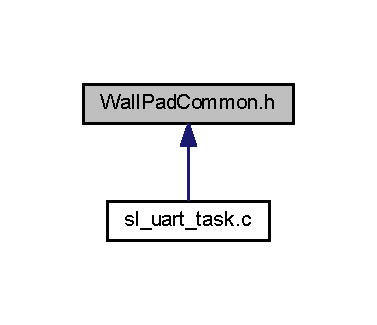
\includegraphics[width=181pt]{_wall_pad_common_8h__dep__incl}
\end{center}
\end{figure}
\subsection*{데이터 구조}
\begin{DoxyCompactItemize}
\item 
struct \mbox{\hyperlink{struct_st_wall_pad}{St\+Wall\+Pad}}
\begin{DoxyCompactList}\small\item\em Wall\+Pad의 접속 ssid 와 pw, mode state를 기록하는 구조체 \end{DoxyCompactList}\item 
struct \mbox{\hyperlink{struct_st_ap_list}{St\+Ap\+List}}
\begin{DoxyCompactList}\small\item\em 주변 검색된 A\+P리스트의 정보를 담는 구조체 (암호화 여부와 수신세기를 포함) \end{DoxyCompactList}\item 
struct \mbox{\hyperlink{struct_st_last_send}{St\+Last\+Send}}
\begin{DoxyCompactList}\small\item\em 업로드가 너무 자주일어나 과금에 영향을 주므로,~\newline
마지막 업로드의 checksum 과 온도정보를 저장하여, aws 에 업로드 주기를 조절하는 구조체 \end{DoxyCompactList}\end{DoxyCompactItemize}
\subsection*{매크로}
\begin{DoxyCompactItemize}
\item 
\#define \mbox{\hyperlink{_wall_pad_common_8h_aa1bfef2ce53d431c709ee094aa02ccb6}{n\+M\+A\+X\+\_\+\+N\+A\+ME}}~40
\item 
\#define \mbox{\hyperlink{_wall_pad_common_8h_a633363122e0b4c2005649a1664a2335a}{n\+M\+A\+X\+\_\+\+I\+N\+I\+T\+\_\+\+C\+HK}}~40
\item 
\#define \mbox{\hyperlink{_wall_pad_common_8h_ac370fa01d5773341bbcc501c01c11d1e}{n\+M\+A\+X\+\_\+\+S\+E\+A\+R\+C\+H\+\_\+\+AP}}~30
\end{DoxyCompactItemize}
\subsection*{타입정의}
\begin{DoxyCompactItemize}
\item 
typedef enum \mbox{\hyperlink{_wall_pad_common_8h_a01baed20aab6218b9846cc7c935f8de9}{typedef\+M\+O\+DE}} \mbox{\hyperlink{_wall_pad_common_8h_a066235770a533eb740dc3fd2494d64da}{e\+M\+O\+DE}}
\item 
typedef struct \mbox{\hyperlink{struct_st_wall_pad}{St\+Wall\+Pad}} \mbox{\hyperlink{_wall_pad_common_8h_afc78910c4749fa1230e1149115f9d70a}{Wall\+Pad}}
\begin{DoxyCompactList}\small\item\em Wall\+Pad의 접속 ssid 와 pw, mode state를 기록하는 구조체 \end{DoxyCompactList}\item 
typedef struct \mbox{\hyperlink{struct_st_wall_pad}{St\+Wall\+Pad}} $\ast$ \mbox{\hyperlink{_wall_pad_common_8h_aadb492147a743663071ec68a774dbb1b}{p\+Wall\+Pad}}
\item 
typedef struct \mbox{\hyperlink{struct_st_ap_list}{St\+Ap\+List}} \mbox{\hyperlink{_wall_pad_common_8h_aa98442922a779292a101450d76255385}{Ap\+List}}
\begin{DoxyCompactList}\small\item\em 주변 검색된 A\+P리스트의 정보를 담는 구조체 (암호화 여부와 수신세기를 포함) \end{DoxyCompactList}\item 
typedef struct \mbox{\hyperlink{struct_st_ap_list}{St\+Ap\+List}} $\ast$ \mbox{\hyperlink{_wall_pad_common_8h_ad2d28182118d0dc42728639623d2dc40}{p\+Ap\+List}}
\item 
typedef struct \mbox{\hyperlink{struct_st_last_send}{St\+Last\+Send}} \mbox{\hyperlink{_wall_pad_common_8h_a78ff28de5f4a28ca30a16c6e0f7b0d35}{Last\+Send}}
\begin{DoxyCompactList}\small\item\em 업로드가 너무 자주일어나 과금에 영향을 주므로,~\newline
마지막 업로드의 checksum 과 온도정보를 저장하여, aws 에 업로드 주기를 조절하는 구조체 \end{DoxyCompactList}\item 
typedef struct \mbox{\hyperlink{struct_st_last_send}{St\+Last\+Send}} $\ast$ \mbox{\hyperlink{_wall_pad_common_8h_ae1755d3e214b69cfb5e3a3e7c7f28516}{p\+Last\+Send}}
\end{DoxyCompactItemize}
\subsection*{열거형 타입}
\begin{DoxyCompactItemize}
\item 
enum \mbox{\hyperlink{_wall_pad_common_8h_a01baed20aab6218b9846cc7c935f8de9}{typedef\+M\+O\+DE}} \{ \newline
\mbox{\hyperlink{_wall_pad_common_8h_a01baed20aab6218b9846cc7c935f8de9abb51c808160be71ef81bc5880610bedc}{e\+M\+O\+D\+E\+\_\+\+N\+O\+NE}} = 0, 
\mbox{\hyperlink{_wall_pad_common_8h_a01baed20aab6218b9846cc7c935f8de9afbc0f8c6a5b25b698265ad7b74b9d9b7}{e\+M\+O\+D\+E\+\_\+\+S\+E\+A\+R\+C\+H\+\_\+\+AP}}, 
\mbox{\hyperlink{_wall_pad_common_8h_a01baed20aab6218b9846cc7c935f8de9a1f5cc10773bdfbec3b85c915572c4d8d}{e\+M\+O\+D\+E\+\_\+\+AP}}, 
\mbox{\hyperlink{_wall_pad_common_8h_a01baed20aab6218b9846cc7c935f8de9ae9734b024c572803a9131d2df41dece2}{e\+M\+O\+D\+E\+\_\+\+C\+O\+N\+N\+E\+CT}}, 
\newline
\mbox{\hyperlink{_wall_pad_common_8h_a01baed20aab6218b9846cc7c935f8de9a25a620c7255a0d3a02bf847826791ce2}{e\+M\+O\+D\+E\+\_\+\+N\+O\+R\+M\+AL}}
 \}
\end{DoxyCompactItemize}


\subsection{매크로 문서화}
\mbox{\Hypertarget{_wall_pad_common_8h_a633363122e0b4c2005649a1664a2335a}\label{_wall_pad_common_8h_a633363122e0b4c2005649a1664a2335a}} 
\index{Wall\+Pad\+Common.\+h@{Wall\+Pad\+Common.\+h}!n\+M\+A\+X\+\_\+\+I\+N\+I\+T\+\_\+\+C\+HK@{n\+M\+A\+X\+\_\+\+I\+N\+I\+T\+\_\+\+C\+HK}}
\index{n\+M\+A\+X\+\_\+\+I\+N\+I\+T\+\_\+\+C\+HK@{n\+M\+A\+X\+\_\+\+I\+N\+I\+T\+\_\+\+C\+HK}!Wall\+Pad\+Common.\+h@{Wall\+Pad\+Common.\+h}}
\subsubsection{\texorpdfstring{n\+M\+A\+X\+\_\+\+I\+N\+I\+T\+\_\+\+C\+HK}{nMAX\_INIT\_CHK}}
{\footnotesize\ttfamily \#define n\+M\+A\+X\+\_\+\+I\+N\+I\+T\+\_\+\+C\+HK~40}



Wall\+Pad\+Common.\+h 파일의 3 번째 라인에서 정의되었습니다.

\mbox{\Hypertarget{_wall_pad_common_8h_aa1bfef2ce53d431c709ee094aa02ccb6}\label{_wall_pad_common_8h_aa1bfef2ce53d431c709ee094aa02ccb6}} 
\index{Wall\+Pad\+Common.\+h@{Wall\+Pad\+Common.\+h}!n\+M\+A\+X\+\_\+\+N\+A\+ME@{n\+M\+A\+X\+\_\+\+N\+A\+ME}}
\index{n\+M\+A\+X\+\_\+\+N\+A\+ME@{n\+M\+A\+X\+\_\+\+N\+A\+ME}!Wall\+Pad\+Common.\+h@{Wall\+Pad\+Common.\+h}}
\subsubsection{\texorpdfstring{n\+M\+A\+X\+\_\+\+N\+A\+ME}{nMAX\_NAME}}
{\footnotesize\ttfamily \#define n\+M\+A\+X\+\_\+\+N\+A\+ME~40}



Wall\+Pad\+Common.\+h 파일의 2 번째 라인에서 정의되었습니다.

\mbox{\Hypertarget{_wall_pad_common_8h_ac370fa01d5773341bbcc501c01c11d1e}\label{_wall_pad_common_8h_ac370fa01d5773341bbcc501c01c11d1e}} 
\index{Wall\+Pad\+Common.\+h@{Wall\+Pad\+Common.\+h}!n\+M\+A\+X\+\_\+\+S\+E\+A\+R\+C\+H\+\_\+\+AP@{n\+M\+A\+X\+\_\+\+S\+E\+A\+R\+C\+H\+\_\+\+AP}}
\index{n\+M\+A\+X\+\_\+\+S\+E\+A\+R\+C\+H\+\_\+\+AP@{n\+M\+A\+X\+\_\+\+S\+E\+A\+R\+C\+H\+\_\+\+AP}!Wall\+Pad\+Common.\+h@{Wall\+Pad\+Common.\+h}}
\subsubsection{\texorpdfstring{n\+M\+A\+X\+\_\+\+S\+E\+A\+R\+C\+H\+\_\+\+AP}{nMAX\_SEARCH\_AP}}
{\footnotesize\ttfamily \#define n\+M\+A\+X\+\_\+\+S\+E\+A\+R\+C\+H\+\_\+\+AP~30}



Wall\+Pad\+Common.\+h 파일의 31 번째 라인에서 정의되었습니다.



\subsection{타입정의 문서화}
\mbox{\Hypertarget{_wall_pad_common_8h_aa98442922a779292a101450d76255385}\label{_wall_pad_common_8h_aa98442922a779292a101450d76255385}} 
\index{Wall\+Pad\+Common.\+h@{Wall\+Pad\+Common.\+h}!Ap\+List@{Ap\+List}}
\index{Ap\+List@{Ap\+List}!Wall\+Pad\+Common.\+h@{Wall\+Pad\+Common.\+h}}
\subsubsection{\texorpdfstring{Ap\+List}{ApList}}
{\footnotesize\ttfamily typedef struct \mbox{\hyperlink{struct_st_ap_list}{St\+Ap\+List}}  \mbox{\hyperlink{_wall_pad_common_8h_aa98442922a779292a101450d76255385}{Ap\+List}}}



주변 검색된 A\+P리스트의 정보를 담는 구조체 (암호화 여부와 수신세기를 포함) 

\mbox{\Hypertarget{_wall_pad_common_8h_a066235770a533eb740dc3fd2494d64da}\label{_wall_pad_common_8h_a066235770a533eb740dc3fd2494d64da}} 
\index{Wall\+Pad\+Common.\+h@{Wall\+Pad\+Common.\+h}!e\+M\+O\+DE@{e\+M\+O\+DE}}
\index{e\+M\+O\+DE@{e\+M\+O\+DE}!Wall\+Pad\+Common.\+h@{Wall\+Pad\+Common.\+h}}
\subsubsection{\texorpdfstring{e\+M\+O\+DE}{eMODE}}
{\footnotesize\ttfamily typedef enum \mbox{\hyperlink{_wall_pad_common_8h_a01baed20aab6218b9846cc7c935f8de9}{typedef\+M\+O\+DE}}  \mbox{\hyperlink{_wall_pad_common_8h_a066235770a533eb740dc3fd2494d64da}{e\+M\+O\+DE}}}

\mbox{\Hypertarget{_wall_pad_common_8h_a78ff28de5f4a28ca30a16c6e0f7b0d35}\label{_wall_pad_common_8h_a78ff28de5f4a28ca30a16c6e0f7b0d35}} 
\index{Wall\+Pad\+Common.\+h@{Wall\+Pad\+Common.\+h}!Last\+Send@{Last\+Send}}
\index{Last\+Send@{Last\+Send}!Wall\+Pad\+Common.\+h@{Wall\+Pad\+Common.\+h}}
\subsubsection{\texorpdfstring{Last\+Send}{LastSend}}
{\footnotesize\ttfamily typedef struct \mbox{\hyperlink{struct_st_last_send}{St\+Last\+Send}} \mbox{\hyperlink{_wall_pad_common_8h_a78ff28de5f4a28ca30a16c6e0f7b0d35}{Last\+Send}}}



업로드가 너무 자주일어나 과금에 영향을 주므로,~\newline
마지막 업로드의 checksum 과 온도정보를 저장하여, aws 에 업로드 주기를 조절하는 구조체 

\mbox{\Hypertarget{_wall_pad_common_8h_ad2d28182118d0dc42728639623d2dc40}\label{_wall_pad_common_8h_ad2d28182118d0dc42728639623d2dc40}} 
\index{Wall\+Pad\+Common.\+h@{Wall\+Pad\+Common.\+h}!p\+Ap\+List@{p\+Ap\+List}}
\index{p\+Ap\+List@{p\+Ap\+List}!Wall\+Pad\+Common.\+h@{Wall\+Pad\+Common.\+h}}
\subsubsection{\texorpdfstring{p\+Ap\+List}{pApList}}
{\footnotesize\ttfamily typedef struct \mbox{\hyperlink{struct_st_ap_list}{St\+Ap\+List}} $\ast$ \mbox{\hyperlink{_wall_pad_common_8h_ad2d28182118d0dc42728639623d2dc40}{p\+Ap\+List}}}

\mbox{\Hypertarget{_wall_pad_common_8h_ae1755d3e214b69cfb5e3a3e7c7f28516}\label{_wall_pad_common_8h_ae1755d3e214b69cfb5e3a3e7c7f28516}} 
\index{Wall\+Pad\+Common.\+h@{Wall\+Pad\+Common.\+h}!p\+Last\+Send@{p\+Last\+Send}}
\index{p\+Last\+Send@{p\+Last\+Send}!Wall\+Pad\+Common.\+h@{Wall\+Pad\+Common.\+h}}
\subsubsection{\texorpdfstring{p\+Last\+Send}{pLastSend}}
{\footnotesize\ttfamily typedef struct \mbox{\hyperlink{struct_st_last_send}{St\+Last\+Send}} $\ast$ \mbox{\hyperlink{_wall_pad_common_8h_ae1755d3e214b69cfb5e3a3e7c7f28516}{p\+Last\+Send}}}

\mbox{\Hypertarget{_wall_pad_common_8h_aadb492147a743663071ec68a774dbb1b}\label{_wall_pad_common_8h_aadb492147a743663071ec68a774dbb1b}} 
\index{Wall\+Pad\+Common.\+h@{Wall\+Pad\+Common.\+h}!p\+Wall\+Pad@{p\+Wall\+Pad}}
\index{p\+Wall\+Pad@{p\+Wall\+Pad}!Wall\+Pad\+Common.\+h@{Wall\+Pad\+Common.\+h}}
\subsubsection{\texorpdfstring{p\+Wall\+Pad}{pWallPad}}
{\footnotesize\ttfamily typedef struct \mbox{\hyperlink{struct_st_wall_pad}{St\+Wall\+Pad}} $\ast$ \mbox{\hyperlink{_wall_pad_common_8h_aadb492147a743663071ec68a774dbb1b}{p\+Wall\+Pad}}}

\mbox{\Hypertarget{_wall_pad_common_8h_afc78910c4749fa1230e1149115f9d70a}\label{_wall_pad_common_8h_afc78910c4749fa1230e1149115f9d70a}} 
\index{Wall\+Pad\+Common.\+h@{Wall\+Pad\+Common.\+h}!Wall\+Pad@{Wall\+Pad}}
\index{Wall\+Pad@{Wall\+Pad}!Wall\+Pad\+Common.\+h@{Wall\+Pad\+Common.\+h}}
\subsubsection{\texorpdfstring{Wall\+Pad}{WallPad}}
{\footnotesize\ttfamily typedef struct \mbox{\hyperlink{struct_st_wall_pad}{St\+Wall\+Pad}}  \mbox{\hyperlink{_wall_pad_common_8h_afc78910c4749fa1230e1149115f9d70a}{Wall\+Pad}}}



Wall\+Pad의 접속 ssid 와 pw, mode state를 기록하는 구조체 



\subsection{열거형 타입 문서화}
\mbox{\Hypertarget{_wall_pad_common_8h_a01baed20aab6218b9846cc7c935f8de9}\label{_wall_pad_common_8h_a01baed20aab6218b9846cc7c935f8de9}} 
\index{Wall\+Pad\+Common.\+h@{Wall\+Pad\+Common.\+h}!typedef\+M\+O\+DE@{typedef\+M\+O\+DE}}
\index{typedef\+M\+O\+DE@{typedef\+M\+O\+DE}!Wall\+Pad\+Common.\+h@{Wall\+Pad\+Common.\+h}}
\subsubsection{\texorpdfstring{typedef\+M\+O\+DE}{typedefMODE}}
{\footnotesize\ttfamily enum \mbox{\hyperlink{_wall_pad_common_8h_a01baed20aab6218b9846cc7c935f8de9}{typedef\+M\+O\+DE}}}

\begin{DoxyEnumFields}{열거형 멤버}
\raisebox{\heightof{T}}[0pt][0pt]{\index{e\+M\+O\+D\+E\+\_\+\+N\+O\+NE@{e\+M\+O\+D\+E\+\_\+\+N\+O\+NE}!Wall\+Pad\+Common.\+h@{Wall\+Pad\+Common.\+h}}\index{Wall\+Pad\+Common.\+h@{Wall\+Pad\+Common.\+h}!e\+M\+O\+D\+E\+\_\+\+N\+O\+NE@{e\+M\+O\+D\+E\+\_\+\+N\+O\+NE}}}\mbox{\Hypertarget{_wall_pad_common_8h_a01baed20aab6218b9846cc7c935f8de9abb51c808160be71ef81bc5880610bedc}\label{_wall_pad_common_8h_a01baed20aab6218b9846cc7c935f8de9abb51c808160be71ef81bc5880610bedc}} 
e\+M\+O\+D\+E\+\_\+\+N\+O\+NE&\\
\hline

\raisebox{\heightof{T}}[0pt][0pt]{\index{e\+M\+O\+D\+E\+\_\+\+S\+E\+A\+R\+C\+H\+\_\+\+AP@{e\+M\+O\+D\+E\+\_\+\+S\+E\+A\+R\+C\+H\+\_\+\+AP}!Wall\+Pad\+Common.\+h@{Wall\+Pad\+Common.\+h}}\index{Wall\+Pad\+Common.\+h@{Wall\+Pad\+Common.\+h}!e\+M\+O\+D\+E\+\_\+\+S\+E\+A\+R\+C\+H\+\_\+\+AP@{e\+M\+O\+D\+E\+\_\+\+S\+E\+A\+R\+C\+H\+\_\+\+AP}}}\mbox{\Hypertarget{_wall_pad_common_8h_a01baed20aab6218b9846cc7c935f8de9afbc0f8c6a5b25b698265ad7b74b9d9b7}\label{_wall_pad_common_8h_a01baed20aab6218b9846cc7c935f8de9afbc0f8c6a5b25b698265ad7b74b9d9b7}} 
e\+M\+O\+D\+E\+\_\+\+S\+E\+A\+R\+C\+H\+\_\+\+AP&\\
\hline

\raisebox{\heightof{T}}[0pt][0pt]{\index{e\+M\+O\+D\+E\+\_\+\+AP@{e\+M\+O\+D\+E\+\_\+\+AP}!Wall\+Pad\+Common.\+h@{Wall\+Pad\+Common.\+h}}\index{Wall\+Pad\+Common.\+h@{Wall\+Pad\+Common.\+h}!e\+M\+O\+D\+E\+\_\+\+AP@{e\+M\+O\+D\+E\+\_\+\+AP}}}\mbox{\Hypertarget{_wall_pad_common_8h_a01baed20aab6218b9846cc7c935f8de9a1f5cc10773bdfbec3b85c915572c4d8d}\label{_wall_pad_common_8h_a01baed20aab6218b9846cc7c935f8de9a1f5cc10773bdfbec3b85c915572c4d8d}} 
e\+M\+O\+D\+E\+\_\+\+AP&\\
\hline

\raisebox{\heightof{T}}[0pt][0pt]{\index{e\+M\+O\+D\+E\+\_\+\+C\+O\+N\+N\+E\+CT@{e\+M\+O\+D\+E\+\_\+\+C\+O\+N\+N\+E\+CT}!Wall\+Pad\+Common.\+h@{Wall\+Pad\+Common.\+h}}\index{Wall\+Pad\+Common.\+h@{Wall\+Pad\+Common.\+h}!e\+M\+O\+D\+E\+\_\+\+C\+O\+N\+N\+E\+CT@{e\+M\+O\+D\+E\+\_\+\+C\+O\+N\+N\+E\+CT}}}\mbox{\Hypertarget{_wall_pad_common_8h_a01baed20aab6218b9846cc7c935f8de9ae9734b024c572803a9131d2df41dece2}\label{_wall_pad_common_8h_a01baed20aab6218b9846cc7c935f8de9ae9734b024c572803a9131d2df41dece2}} 
e\+M\+O\+D\+E\+\_\+\+C\+O\+N\+N\+E\+CT&\\
\hline

\raisebox{\heightof{T}}[0pt][0pt]{\index{e\+M\+O\+D\+E\+\_\+\+N\+O\+R\+M\+AL@{e\+M\+O\+D\+E\+\_\+\+N\+O\+R\+M\+AL}!Wall\+Pad\+Common.\+h@{Wall\+Pad\+Common.\+h}}\index{Wall\+Pad\+Common.\+h@{Wall\+Pad\+Common.\+h}!e\+M\+O\+D\+E\+\_\+\+N\+O\+R\+M\+AL@{e\+M\+O\+D\+E\+\_\+\+N\+O\+R\+M\+AL}}}\mbox{\Hypertarget{_wall_pad_common_8h_a01baed20aab6218b9846cc7c935f8de9a25a620c7255a0d3a02bf847826791ce2}\label{_wall_pad_common_8h_a01baed20aab6218b9846cc7c935f8de9a25a620c7255a0d3a02bf847826791ce2}} 
e\+M\+O\+D\+E\+\_\+\+N\+O\+R\+M\+AL&\\
\hline

\end{DoxyEnumFields}


Wall\+Pad\+Common.\+h 파일의 7 번째 라인에서 정의되었습니다.


\begin{DoxyCode}
8 \{
9   \mbox{\hyperlink{_wall_pad_common_8h_a01baed20aab6218b9846cc7c935f8de9abb51c808160be71ef81bc5880610bedc}{eMODE\_NONE}}  = 0,  
10   \mbox{\hyperlink{_wall_pad_common_8h_a01baed20aab6218b9846cc7c935f8de9afbc0f8c6a5b25b698265ad7b74b9d9b7}{eMODE\_SEARCH\_AP}},  
11   \mbox{\hyperlink{_wall_pad_common_8h_a01baed20aab6218b9846cc7c935f8de9a1f5cc10773bdfbec3b85c915572c4d8d}{eMODE\_AP}},     \textcolor{comment}{// AP MODE}
12   \mbox{\hyperlink{_wall_pad_common_8h_a01baed20aab6218b9846cc7c935f8de9ae9734b024c572803a9131d2df41dece2}{eMODE\_CONNECT}},    \textcolor{comment}{// Normal }
13   \mbox{\hyperlink{_wall_pad_common_8h_a01baed20aab6218b9846cc7c935f8de9a25a620c7255a0d3a02bf847826791ce2}{eMODE\_NORMAL}}    \textcolor{comment}{// Normal }
14 \} \mbox{\hyperlink{_wall_pad_common_8h_a066235770a533eb740dc3fd2494d64da}{eMODE}};
\end{DoxyCode}

%--- End generated contents ---

% Index
\backmatter
\newpage
\phantomsection
\clearemptydoublepage
\addcontentsline{toc}{chapter}{색인}
\printindex

\end{document}
